
\chapter[Simulation for the muon EDM search]{Simulation for the muon EDM \\search}\label{chap:5}

% \myworries{What about the fact that the vertical angle has a different width to data???}

% \myworries{Is it OK to refer to "reco vertices" ect in the text?}

The muon EDM search described in this thesis relies on a large-scale Monte Carlo simulation to verify aspects of the theory behind the EDM search, develop the analysis strategy, and study sources of systematic uncertainty. Critically, simulation also provides a means of characterising the impact of detector acceptance on the dilution of observed angle in-phase with the EDM oscillation, $A_{\text{EDM}}$, compared with the laboratory frame tilt angle, $\delta$. Without this, an accurate measurement of a potential muon EDM signal is not possible. This work builds on previous muon EDM simulation efforts at E989 by S. Charity \cite{Charity} and G. Lukicov \cite{Lukicov}.

\section{Simulation with a large injected muon EDM}\label{sec:SimulatingALargeEDM}

The analysis described in this section depends, to a great extent, on access to a large sample of Monte Carlo events with an injected muon EDM of known size. The size of the injected signal was chosen to be $5.4\times10^{-18}$ $e\cdot\text{cm}$, or 30$\times$ the muon EDM upper limit measured at BNL \cite{BNLEDM}. The exact magnitude of the injected signal is somewhat arbitrary, but a large signal is preferable as it may be more easily resolved from a finite number of simulated events. An additional, smaller, sample with an injected muon EDM of $1.8\times10^{-18}$ $e\cdot\text{cm}$, or 10$\times$ the BNL upper limit, was generated for the purposes of cross-checking the main sample. By application of Equation \ref{eqn:EDMFromAngle}, this gives $\delta$ values of 1.69 mrad and 0.594 mrad for the 30$\times$ and 10$\times$ BNL samples respectively. 

Events were generated using the GEANT4-based in-house framework \texttt{gm2ringsim}, introduced in Chapter \ref{chap:3} Section \ref{sec:Computing}, using a mode termed the `gas gun'. In this mode, muon decay times are randomly sampled from an exponentially decaying distribution, while the energy-momentum four-vector, position, and polarisation of the individual muons are determined based on the time since injection. The simulated muons are then placed in a model of the storage ring and allowed to decay instantaneously. A muon EDM is injected by the addition of an oscillating vertical component to the muon polarisation vector \cite{Charity}. 

\begin{table}[t!]
% \begin{adjustwidth}{-1.5em}{}
\centering
\begin{tabular}{l|cc}
\hline
\hline
Label & Description & Decays or vertices [$\times10^{6}$] \\ 
\hline
\textit{All decays} & All $e^{+}$ (100\% acceptance) & $70.6$ \\ 
\textit{Truth/reco vertices} & \makecell{Truth/measured information \\ from track vertices} & $32.9$ \\ 
\hline
\hline
\end{tabular}
% \end{adjustwidth}
\caption{The three simulation reconstructions described in this chapter, including the number of decays, or quality-cut-passing track vertices, for samples with an injected EDM of $5.4\times10^{-18}$ $e\cdot\text{cm}$ ($\sim30$$\times$ the BNL upper limit). Approximately 1\% of generated events (one muon per event) results in high quality track vertex. The \textit{truth/reco vertices} samples are not a subset of \textit{all decays} in this case.} 
\label{tbl:SimSamples}
\end{table}

\begin{figure}[t!]
\centering{}
\subfloat[\textit{All decays}.]{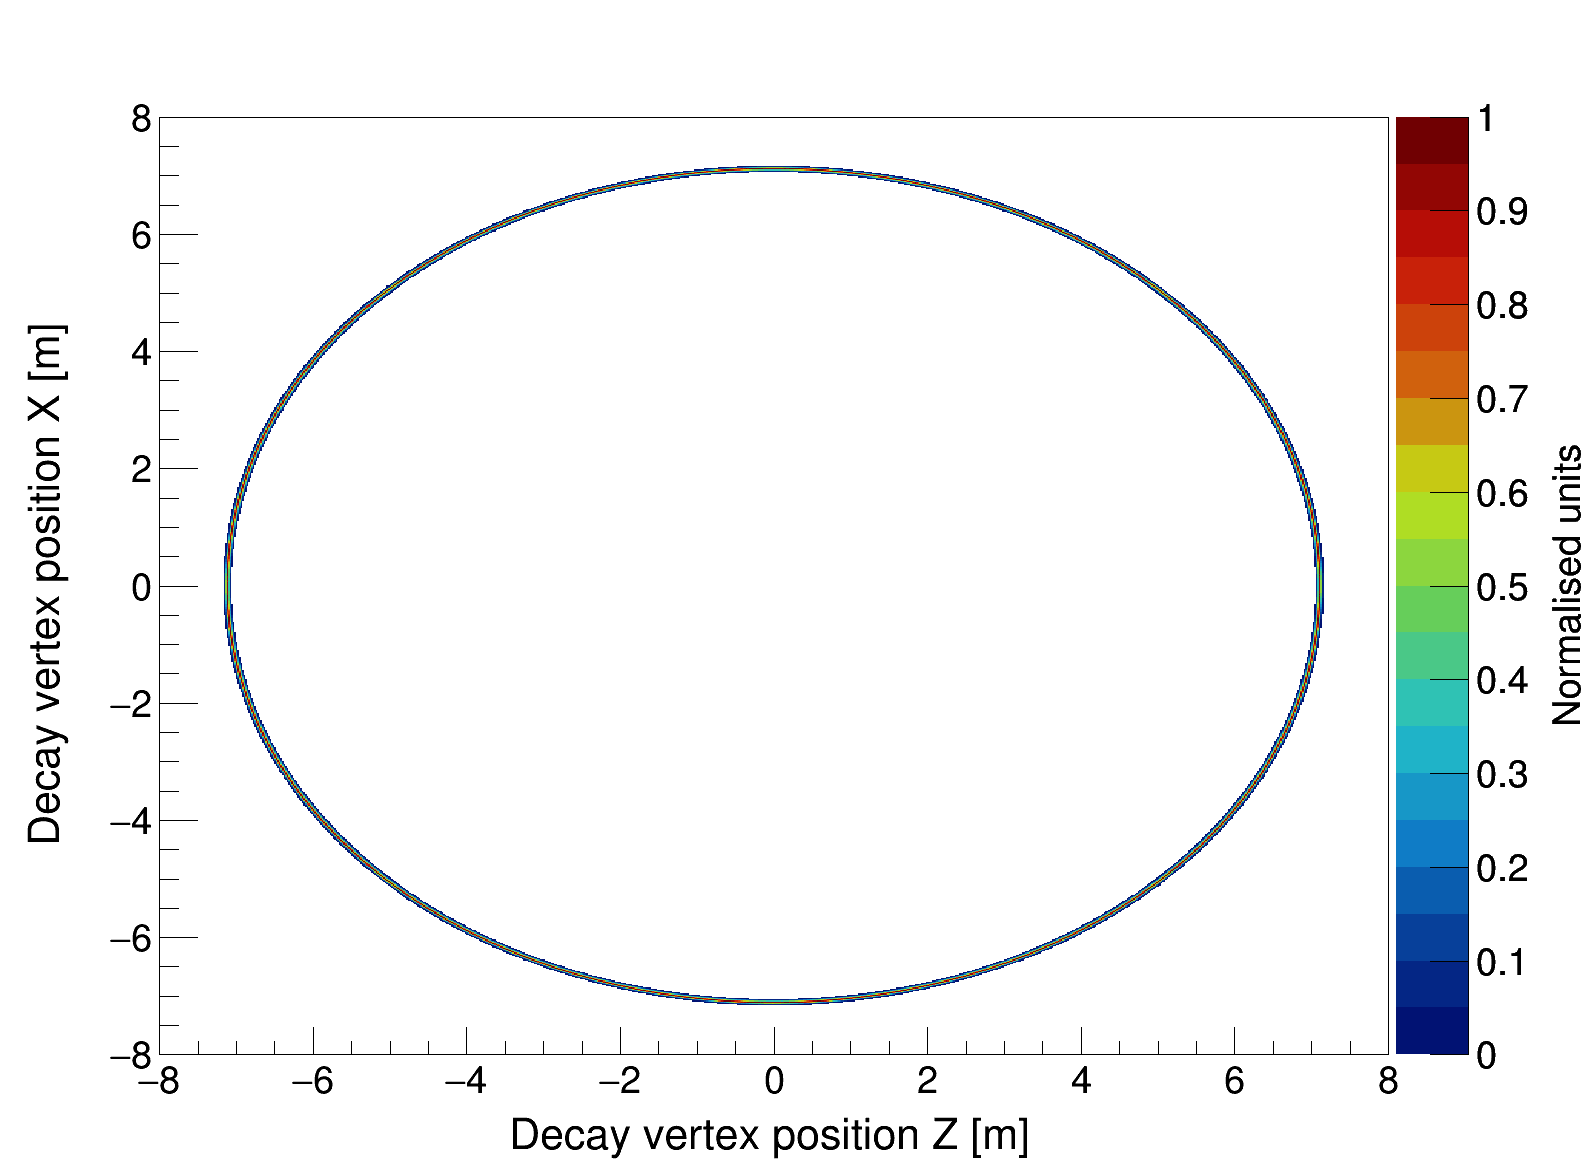
\includegraphics[trim={0 0 0 0},clip,width=.49\textwidth]{Images/Chapter5/allDecays_DecayZ_vs_DecayX.png}\label{subfig:AllDecaysAzimuthalAcceptance}}
\subfloat[\textit{Reco vertices}.]{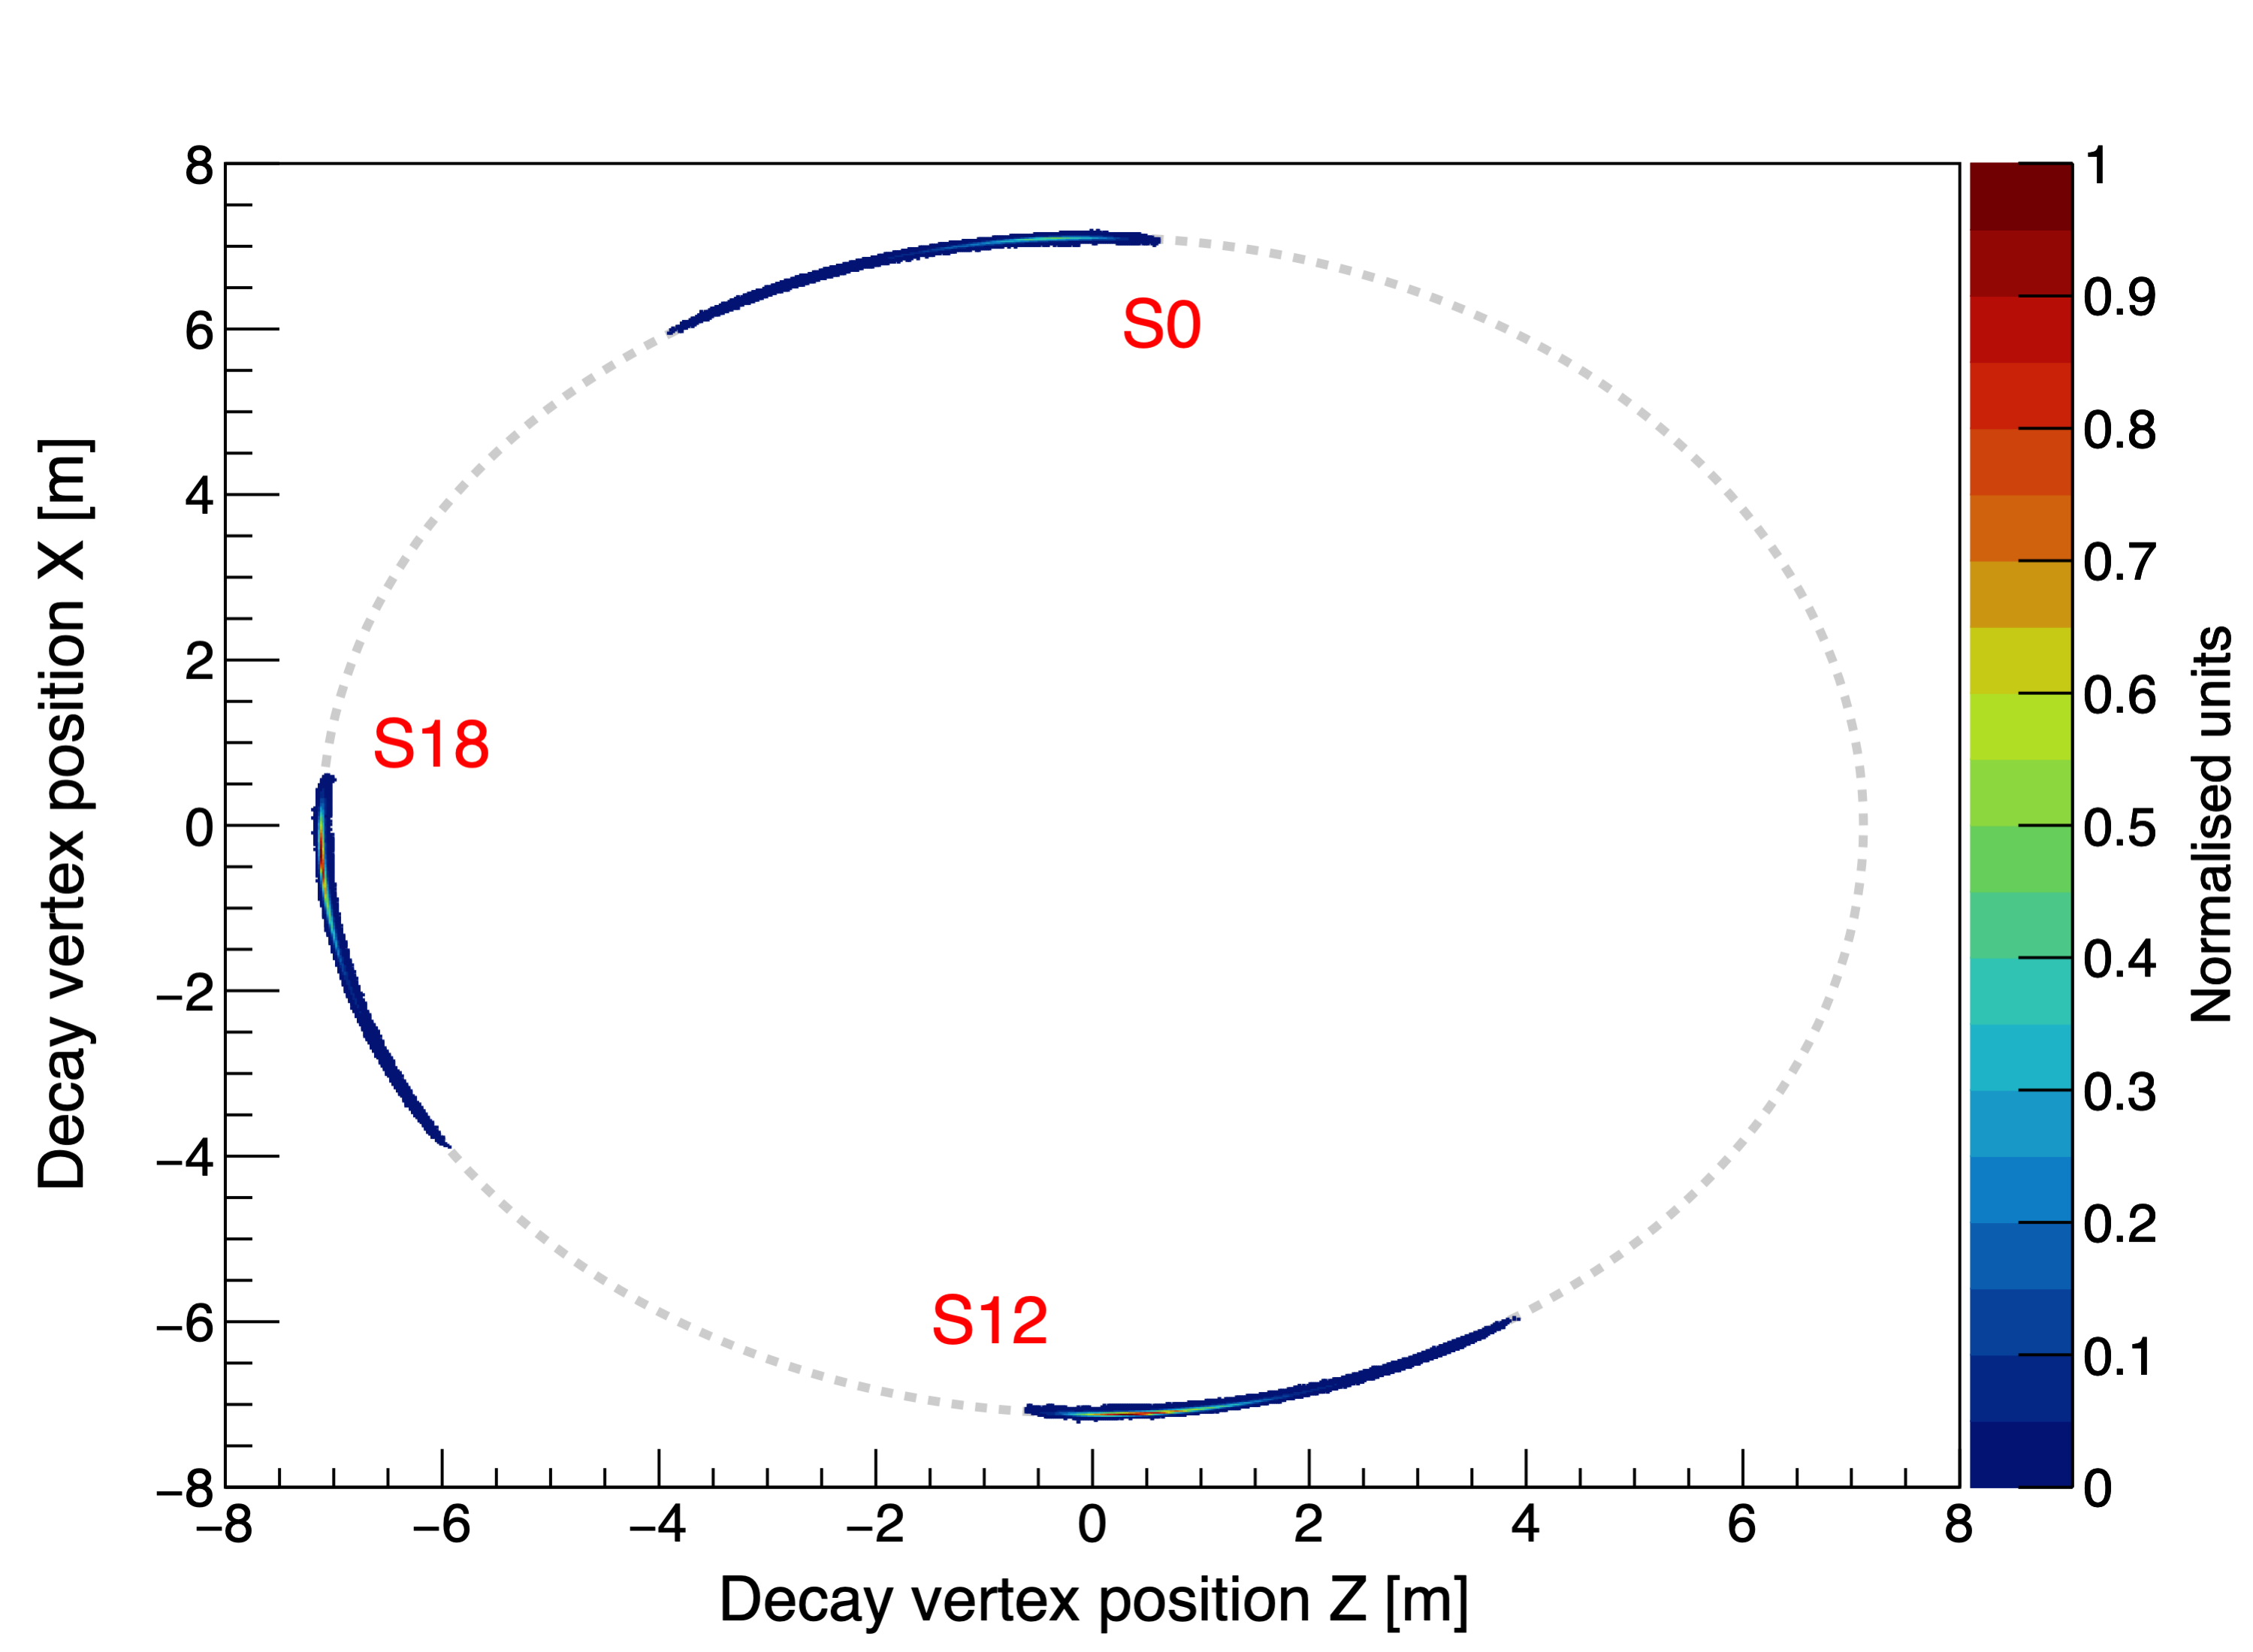
\includegraphics[trim={0 0 0 0},clip,width=.49\textwidth]{Images/Chapter5/S12S18_trackReco_DecayZ_vs_DecayX.png}\label{subfig:TrackRecoAzimuthalAcceptance}}
\caption{The azimuthal acceptance of Monte Carlo events for: (a) truth parameters for all positrons, \textit{all decays}, with 100$\%$ acceptance; (b) measured information from track decay vertices, \textit{reco vertices}, showing a $\sim25\degree$ acceptance. The coordinate system is the same as used in Figure \ref{fig:RingSchematic}, that is, where the inflector is positioned at 12 o'clock with the muons circulating clockwise. The ideal orbit is marked by a grey dashed line, and the positions of each tracker station are indicated. Station 0 (S0) is a proposed third tracker station, which, at present, only exists in simulation.}
\label{fig:SimAzimuthalAcceptance}
\end{figure} 


Once generated, events were reconstructed in three distinct ways: the first, labelled \textit{all decays}, utilised truth decay parameters for all positrons in the sample, with no detector effects; the second, labelled \textit{truth vertices}, used truth information associated with extrapolated track decay vertices; and the third, labelled \textit{reco vertices}\footnote{`Reco' being an abbreviation for `reconstructed', or `measured using the nominal track reconstruction algorithm'.}, used measured information associated with extrapolated track decay vertices. These three reconstructions are summarised in Table \ref{tbl:SimSamples}, along with the number of $e^{+}$ or quality-cut-passing extrapolated track vertices, introduced in Chapter \ref{chap:3} Section \ref{subsec:Trackers}, for the primary 30$\times$ BNL sample. Comparison between decays and vertices was critical when characterising the impact of the detector acceptance on the dilution of the measured tilt angle, expanded upon in Section \ref{sec:AcceptanceSim}. This is because the \textit{all decays} sample provides a means of performing a muon EDM analysis with 100\% acceptance, as demonstrated by the azimuthal acceptance for \textit{all decays} compared with \textit{reco vertices} shown in Figure \ref{fig:SimAzimuthalAcceptance}. 

It should be noted that the samples of decays and track vertices were not reconstructed from entirely the same sets of events, so that one is not a subset of the other. This is because a large sample consisting only of track vertices was generated prior to the decision to retain the decays, and means that the relative number of vertices and decays in Table \ref{tbl:SimSamples} are not a reflection of detector acceptance. The true acceptance of the trackers, in terms of track vertices per decay positron, has been measured to be $\sim$3.5\% (where just $\sim$1\% form high quality track vertices). This is despite the excellent 25$\degree$ azimuthal acceptance per tracker station, which is limited by the fact that the number of positrons is highest at low momentum (below 1 GeV), as illustrated by the number distribution function in Figure \ref{fig:Asymmetry_EDM}, and the average momentum of tracks originating from further upstream are necessarily high momentum -- lower momentum positrons curl out of the storage region before reaching the detector. The low momentum positrons which do pass through the trackers do not generally form good quality tracks due to their high curvature in the magnetic field. Track quality cuts are discussed in Chapter \ref{chap:3} Section \ref{subsec:Trackers}.

% tracker accepts positrons from a  region of the ring, but may be largely attributed to is primarily a consequence of a combination of trackers geometric acceptance and momentum acceptance, where only $\sim$3.5\% of decays form a track (of any sort). This is despite each tracker accepts positrons from a 25$\degree$ azimuthal region of the ring, the average momentum of tracks originating from the furthest point of that arc are necessarily high momentum, where lower momentum decays curl out of the storage region before reaching the detector. In addition, while the number of decays is highest at low momentum (below 1 GeV), as illustrated by the number distribution function in Figure \ref{fig:Asymmetry_EDM}, such decays do not usually form good quality tracks due to their high curvature in the field and a quality requirement on a minimum of twelve tracker planes hit. 

% 
% Once generated, events were reconstructed in three distinct ways: the first, labelled \textit{all decays}, utilised truth decay parameters for all positrons in the sample, with no detector effects; the second, labelled \textit{truth vertices}, used truth information associated with extrapolated track decay vertices; and the third, labelled \textit{reco vertices}\footnote{`Reco' being an abbreviation for `reconstructed', or `measured using the nominal track reconstruction algorithm'.}, used measured information associated with extrapolated track decay vertices. These three reconstructions are summarised in Table \ref{tbl:SimSamples}, along with the number of $e^{+}$ or quality-cut-passing extrapolated track vertices, introduced in Chapter \ref{chap:3} Section \ref{subsec:Trackers}, for the primary 30$\times$ BNL sample. \myworries{It should be noted that a large sample consisting only of track vertices was generated prior to the decision to retain the decays, so the samples of decays and track vertices were not reconstructed from entirely the same sets of events. This means that the relative number of vertices and decays in Table \ref{tbl:SimSamples} are not a reflection of detector acceptance. The true acceptance of the trackers, in terms of high quality track vertices per decay positron, has been measured to be $\sim$1\%. This is despite the excellent 25$\degree$ azimuthal acceptance 

% tracker accepts positrons from a  region of the ring, but may be largely attributed to is primarily a consequence of a combination of trackers geometric acceptance and momentum acceptance, where only $\sim$3.5\% of decays form a track (of any sort). This is despite each tracker accepts positrons from a 25$\degree$ azimuthal region of the ring, the average momentum of tracks originating from the furthest point of that arc are necessarily high momentum, where lower momentum decays curl out of the storage region before reaching the detector. In addition, while the number of decays is highest at low momentum (below 1 GeV), as illustrated by the number distribution function in Figure \ref{fig:Asymmetry_EDM}, such decays do not usually form good quality tracks due to their high curvature in the field and a quality requirement on a minimum of twelve tracker planes hit. In total, the requirements for track quality, discussed in Chapter \ref{chap:3} Section \ref{subsec:Trackers}, reduce the effective acceptance by a further $\sim$60\%.}

% Comparison between decays and vertices was critical when characterising the impact of the detector acceptance on the dilution of the measured tilt angle, expanded upon in Section \ref{sec:AcceptanceSim}. This is because the \textit{all decays} sample provides a means of performing a muon EDM analysis with 100\% acceptance, as demonstrated by the azimuthal acceptance for \textit{all decays} compared with \textit{reco vertices} shown in Figure \ref{fig:SimAzimuthalAcceptance}. 


% in  while each tracker station accepts positrons over a $\sim25\degree$ azimuth, the correlation between distance from the tracker and momentum means that only high momementum decays are likely to reach the detector from the edge $\sim25\degree$ azimuth. Furthermore, the momentum distribution  of the  positrons are highly correlated with momentum (over a What percentage of the ring azimuth do the trackers cover? Mention the momentum acceptance. Track quality cuts as well. This is primarily a consequence.  }

% \afterpage{
% \begin{figure}[t!]
% \centering{}
% \subfloat[All decays.]{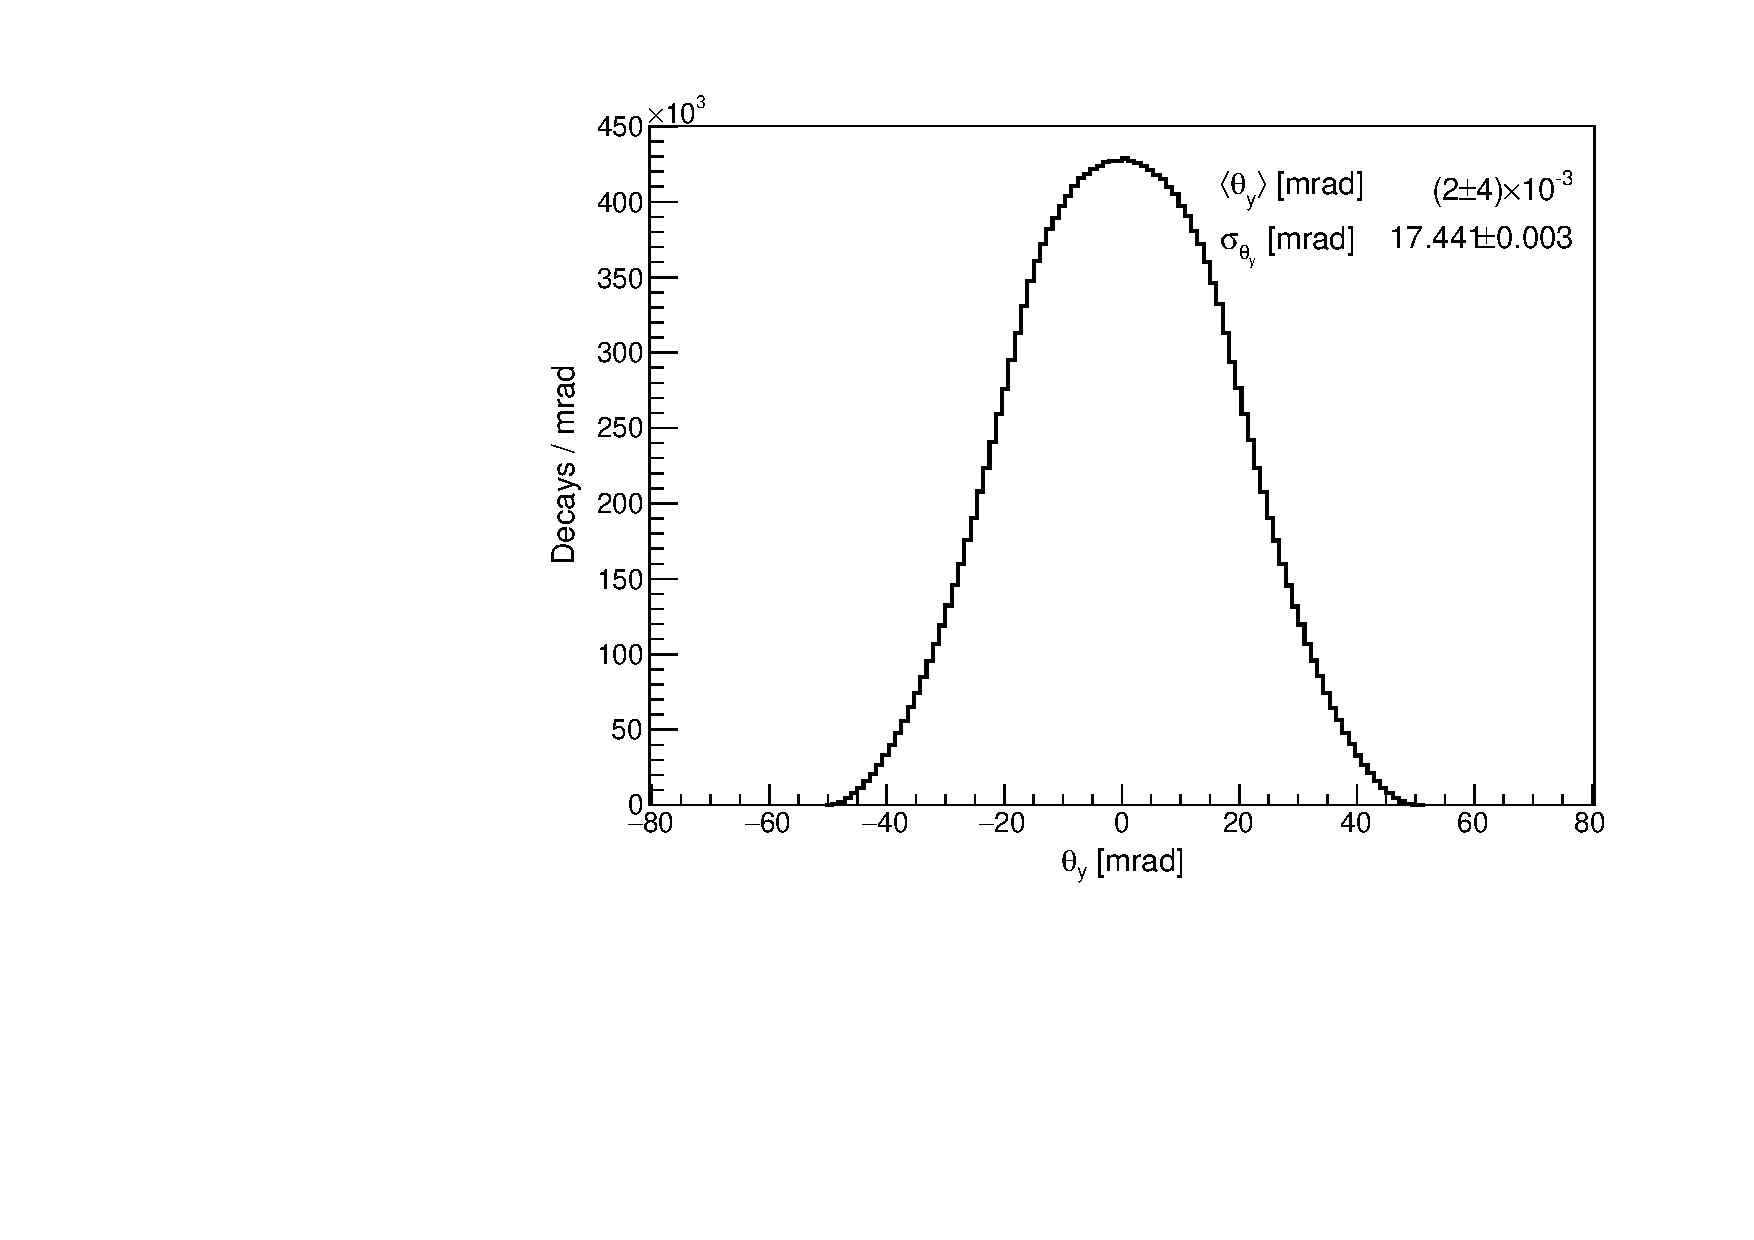
\includegraphics[trim={0 0 0 0},clip,width=.49\textwidth]{Images/Chapter5/ThetaY_AllDecays.pdf}} %\hfill
% % \subfloat[Truth vertices.]{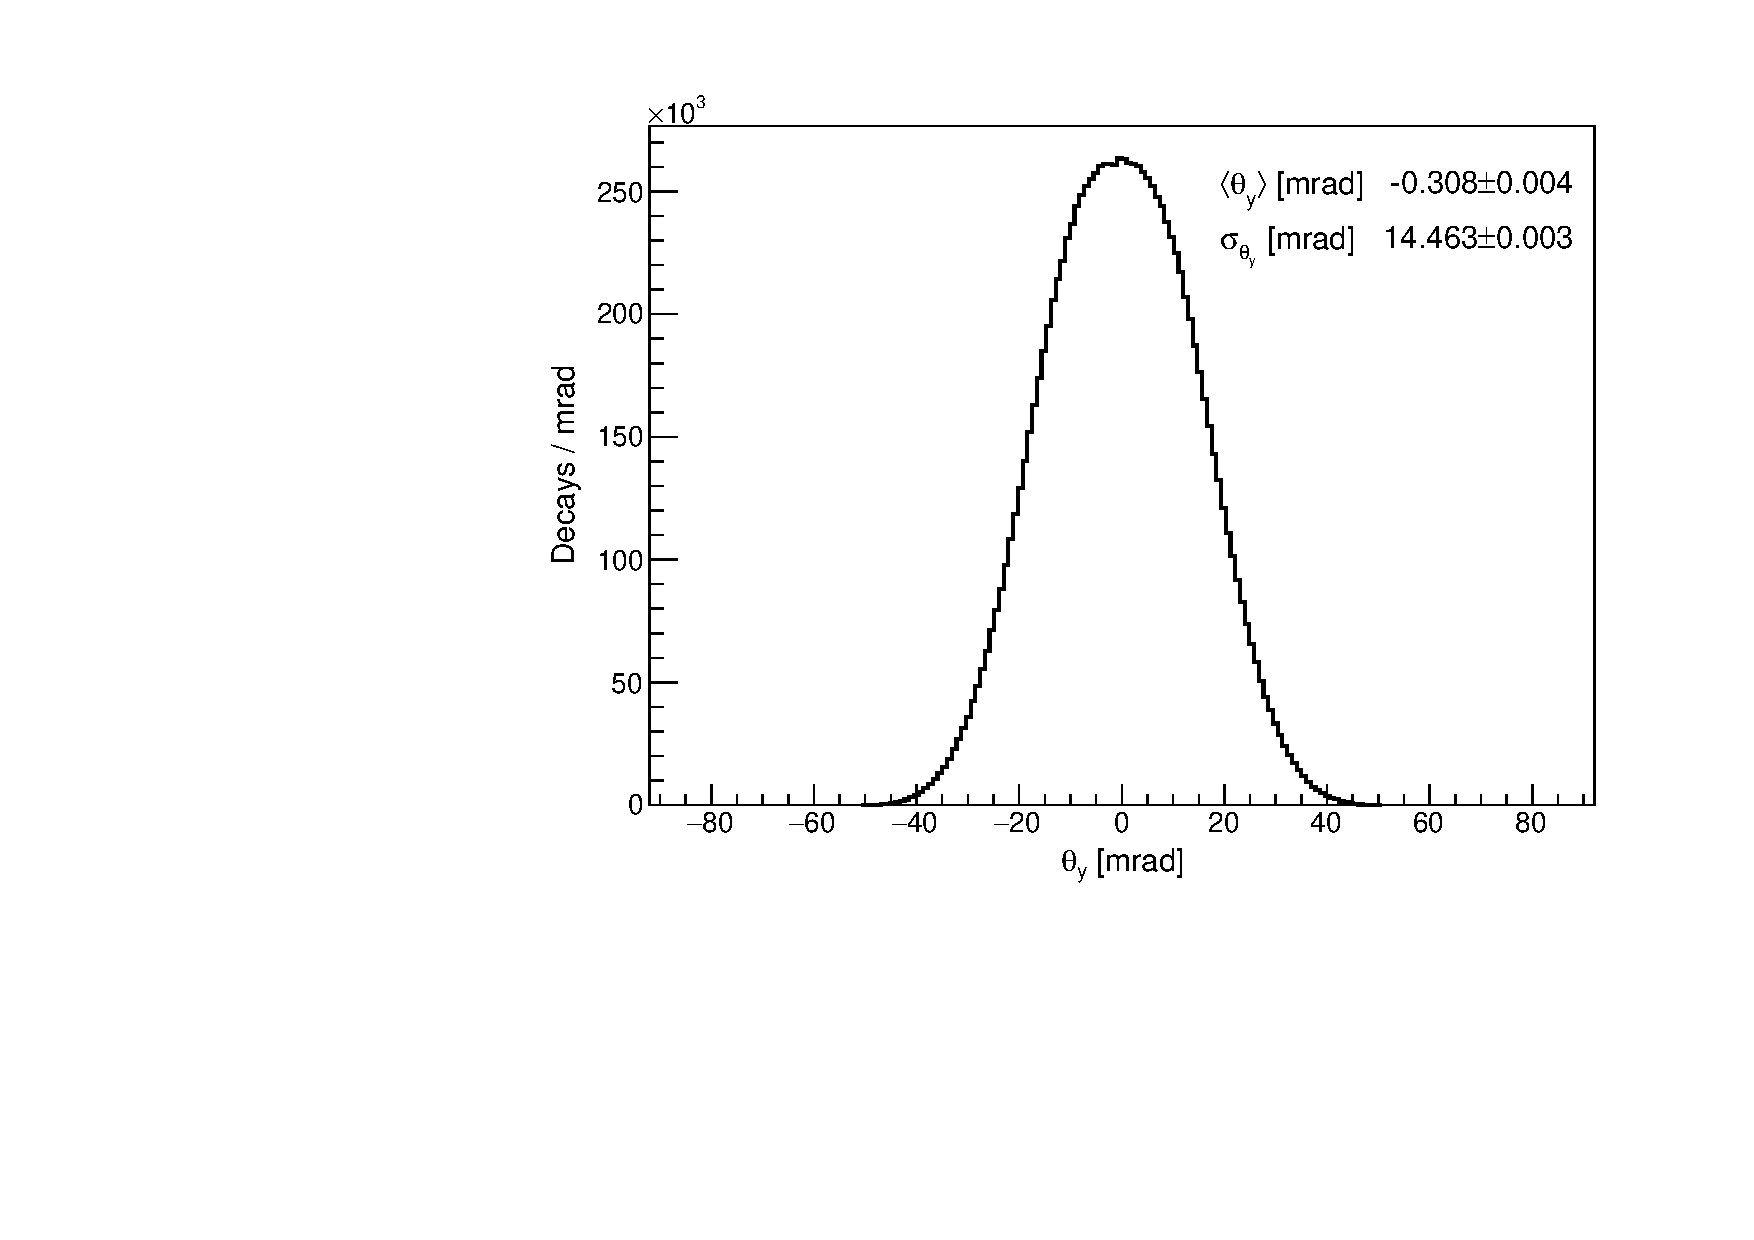
\includegraphics[trim={0 0 0 0},clip,width=.49\textwidth]{Images/Chapter5/ThetaY_TrackTruth.pdf}}
% \subfloat[Reco vertices.]{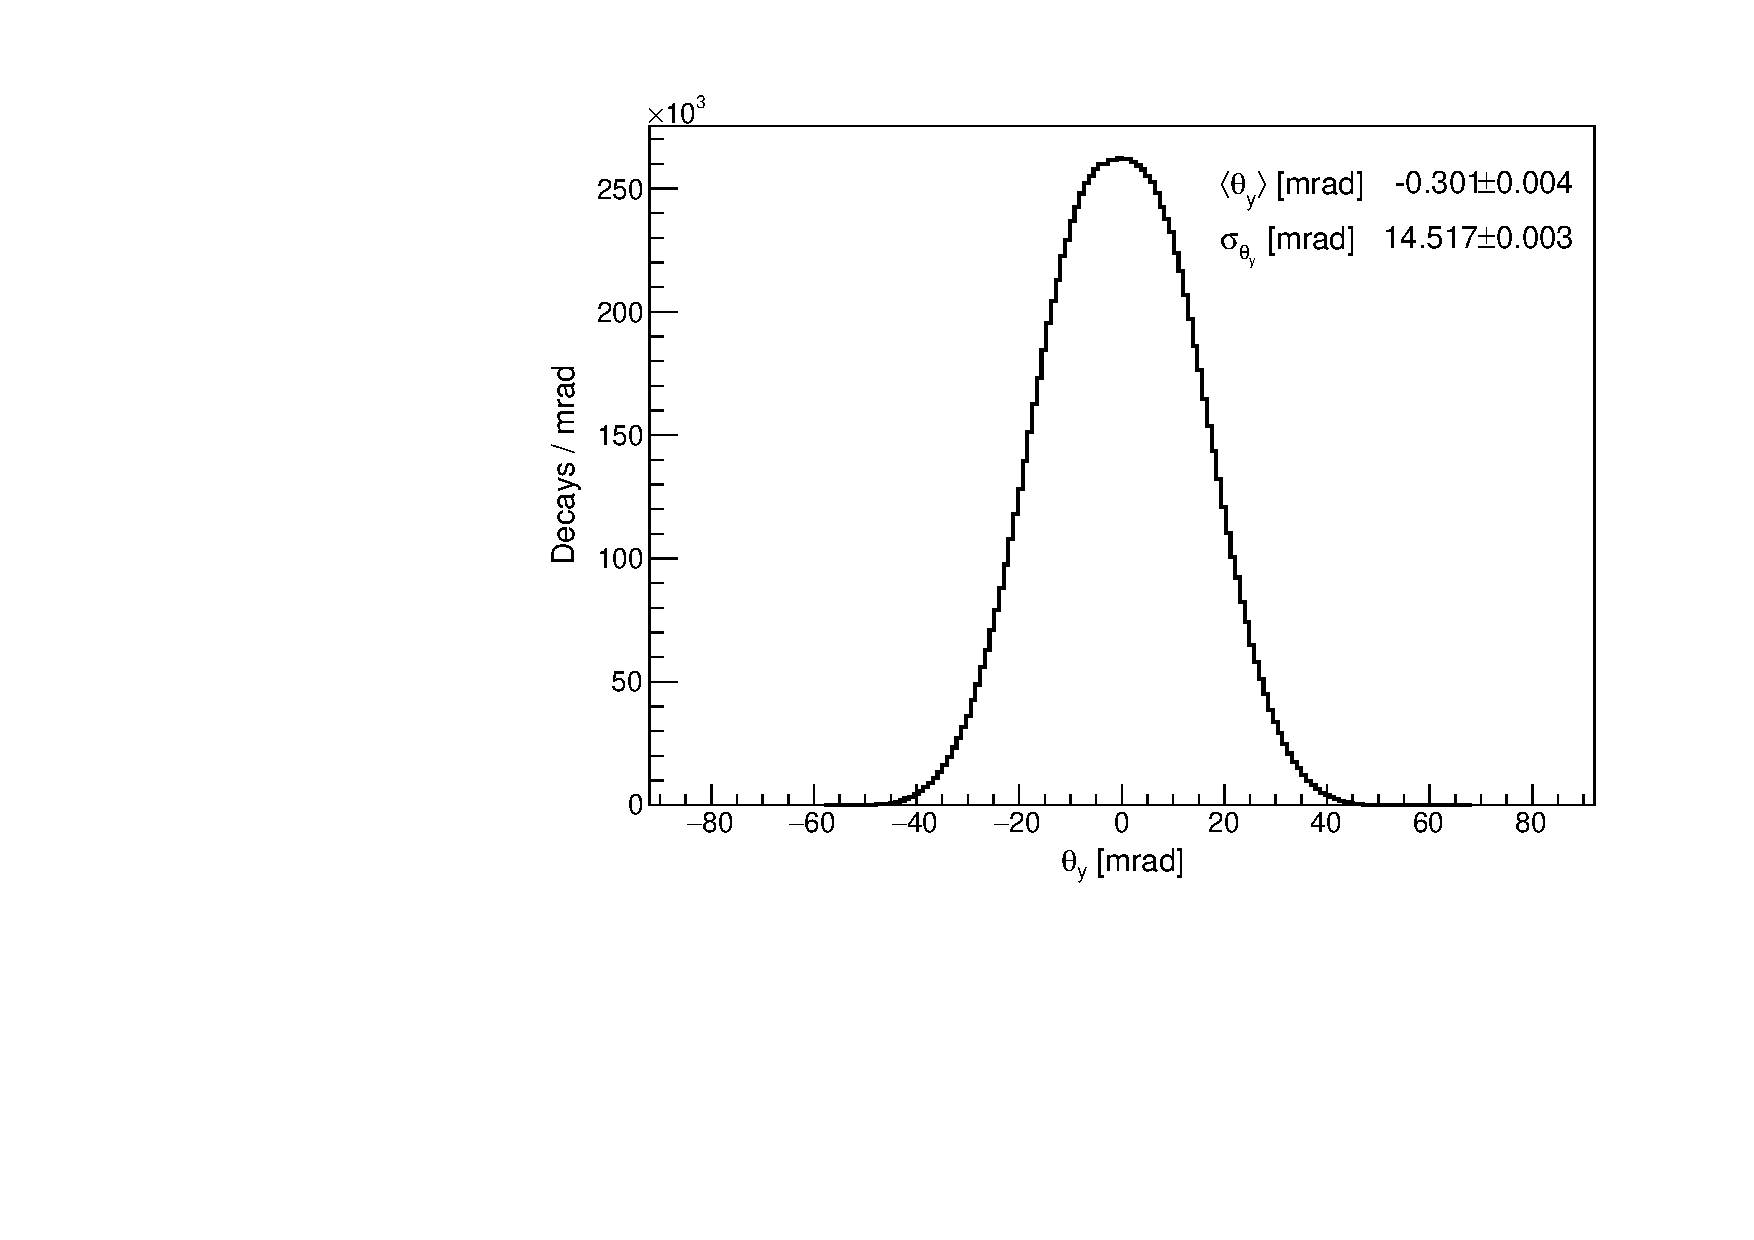
\includegraphics[trim={0 0 0 0},clip,width=.49\textwidth]{Images/Chapter5/ThetaY_TrackReco.pdf}\label{subfig:RecoThetaY}}
% \caption{The vertical decay angle distributions from: (a) truth parameters for all decays in the sample; (b) measured information from track decay vertices. As a consequence of tracker acceptance, the width of the track vertices distribution is reduced compared to all decays, and its mean is offset from zero. \myworries{Link to later section.}}
% \label{fig:SimThetaY}
% \end{figure}  

 

\section{Verifying the decay asymmetry function}\label{sec:DecayAsymVerification}

% \myworries{What about that thing where you divide $A_{\text{EDM}}$ by the RMS?}
A fundamental aspect of the underlying physics driving the experimental sensitivity to an EDM at E989 is the decay asymmetry function, $A(\lambda)$, given by Equation \ref{eqn:AEDM_labFrame} in Chapter \ref{chap:2} Section \ref{subsec:EDMSensitivity}. As such, it is important to verify the validity of this function. This was accomplished by use of the \textit{all decays} sample, where truth information was used to calculate the angle $\epsilon$ between the $x$-$z$ plane and the muon spin polarisation vector, as well as the angle $\theta$ between the $x$-$z$ plane and the decay positron momentum vector. If the product of these angles is positive, so that $\epsilon\cdot\theta > 0$, then the muon spin vector and positron momentum vector must be directed in the same vertical hemisphere, and so these were counted as `up' decays. If $\epsilon\cdot\theta < 0$, then the reverse is true, and such decays were counted as `down' decays. From the numbers of up/down decays, $N_{u}$ and $N_{d}$, it is possible to define the asymmetry as 
%
\begin{equation}
  A = \frac{N_{u}-N_{d}}{N_{u}+N_{d}},
  \label{eqn:UpDownAsym}
\end{equation}
%
with a corresponding uncertainty of 
%sdv
\begin{equation}
  \delta A = \sqrt{\frac{1-A^{2}}{N_{u}+N_{d}}},
  \label{eqn:UpDownAsymError}
\end{equation}
%float eA = sqrt((1-pow(A,2))/(N_1+N_2));
%
a full derivation for which is given in Appendix \ref{app:Unc} Section \ref{app:A}. The distributions $A(\lambda)$ and the statistical figure-of-merit (FOM) $NA^{2}(\lambda)$, derived from simulation, are shown in Figure \ref{subfig:SimEDMAsymDists}. The analytical form of $A(\lambda)$ is overlaid on the corresponding distribution from simulation in Figure \ref{subfig:SimEDMAsymFit}, showing excellent agreement. 

\begin{figure}[t!]
\centering{}
\subfloat[]{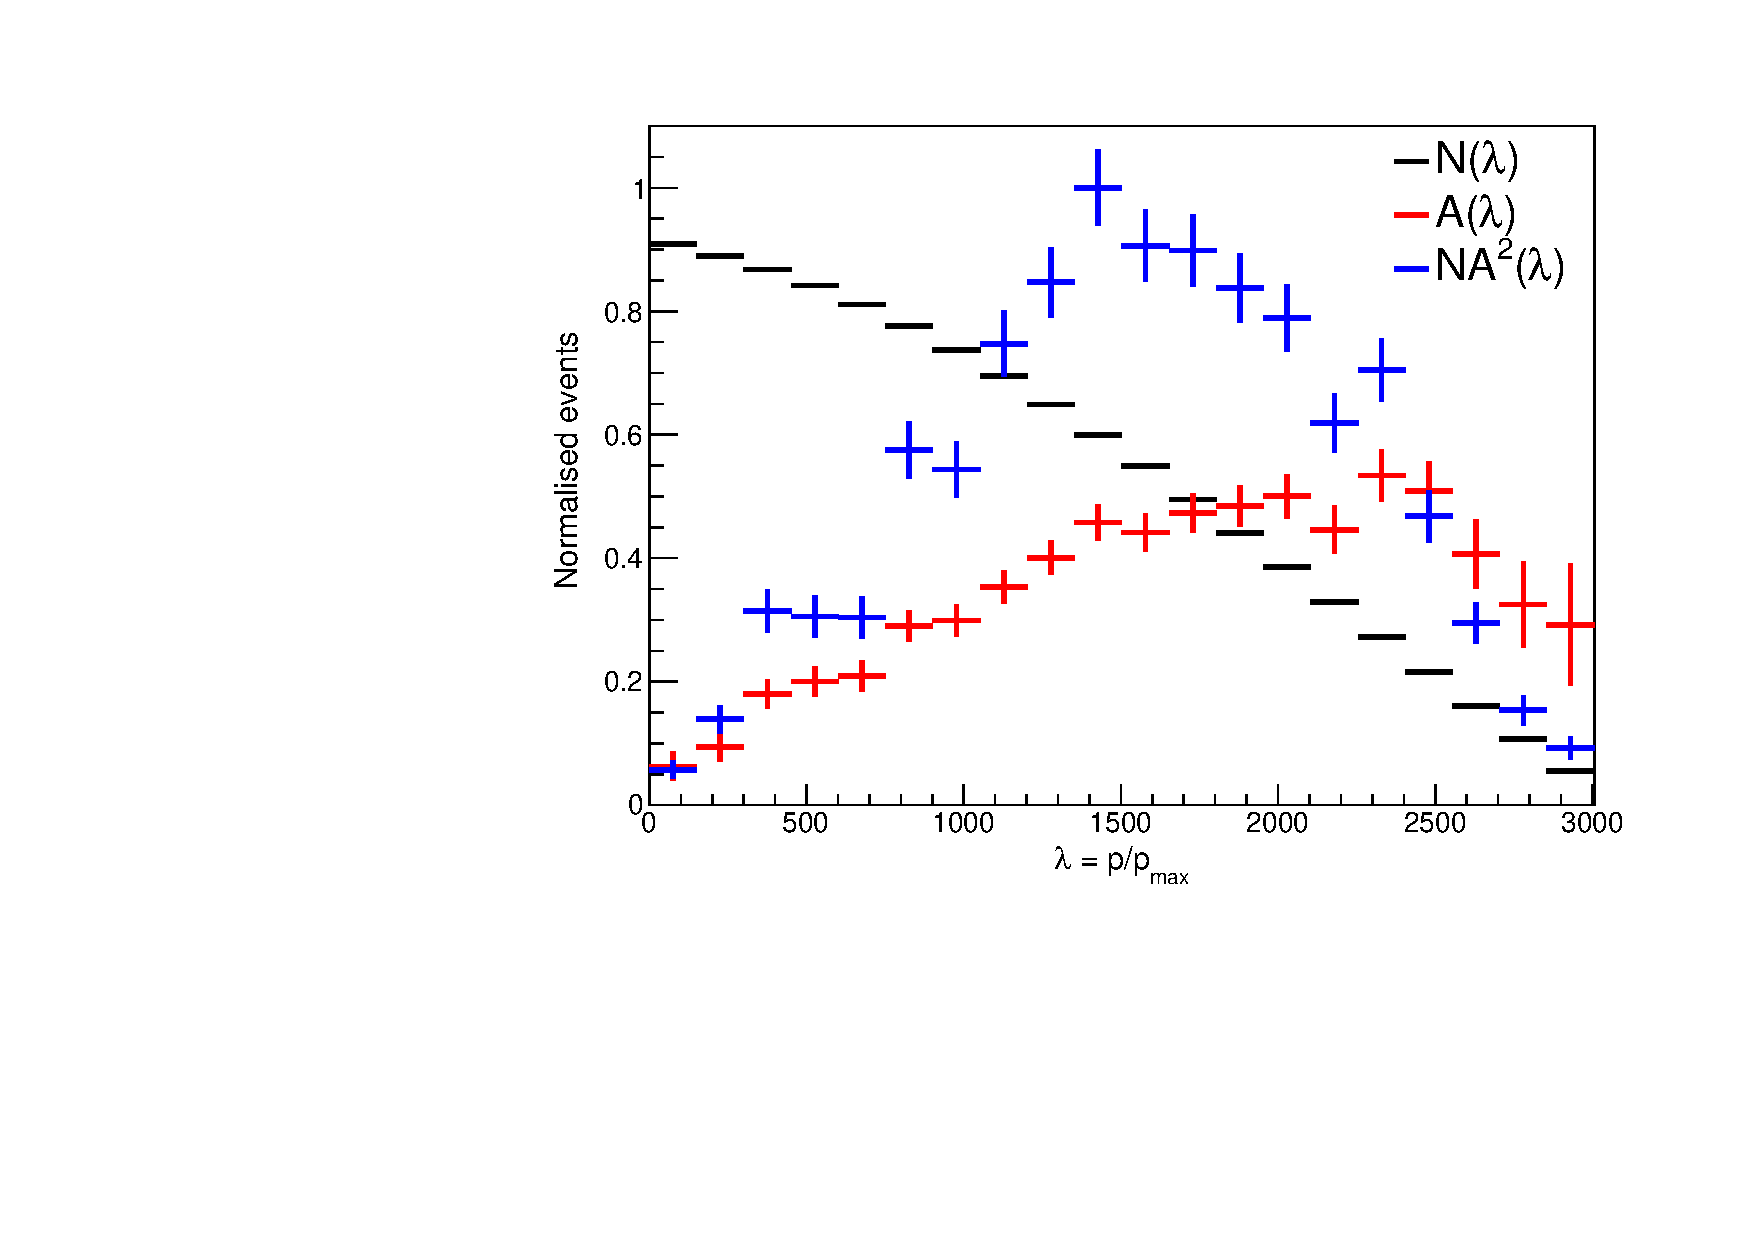
\includegraphics[trim={0 0 0 1cm},clip,width=.49\textwidth]{Images/Chapter5/NormDiffDecayAsymHists_LAB_TEST.pdf}\label{subfig:SimEDMAsymDists}}
\subfloat[]{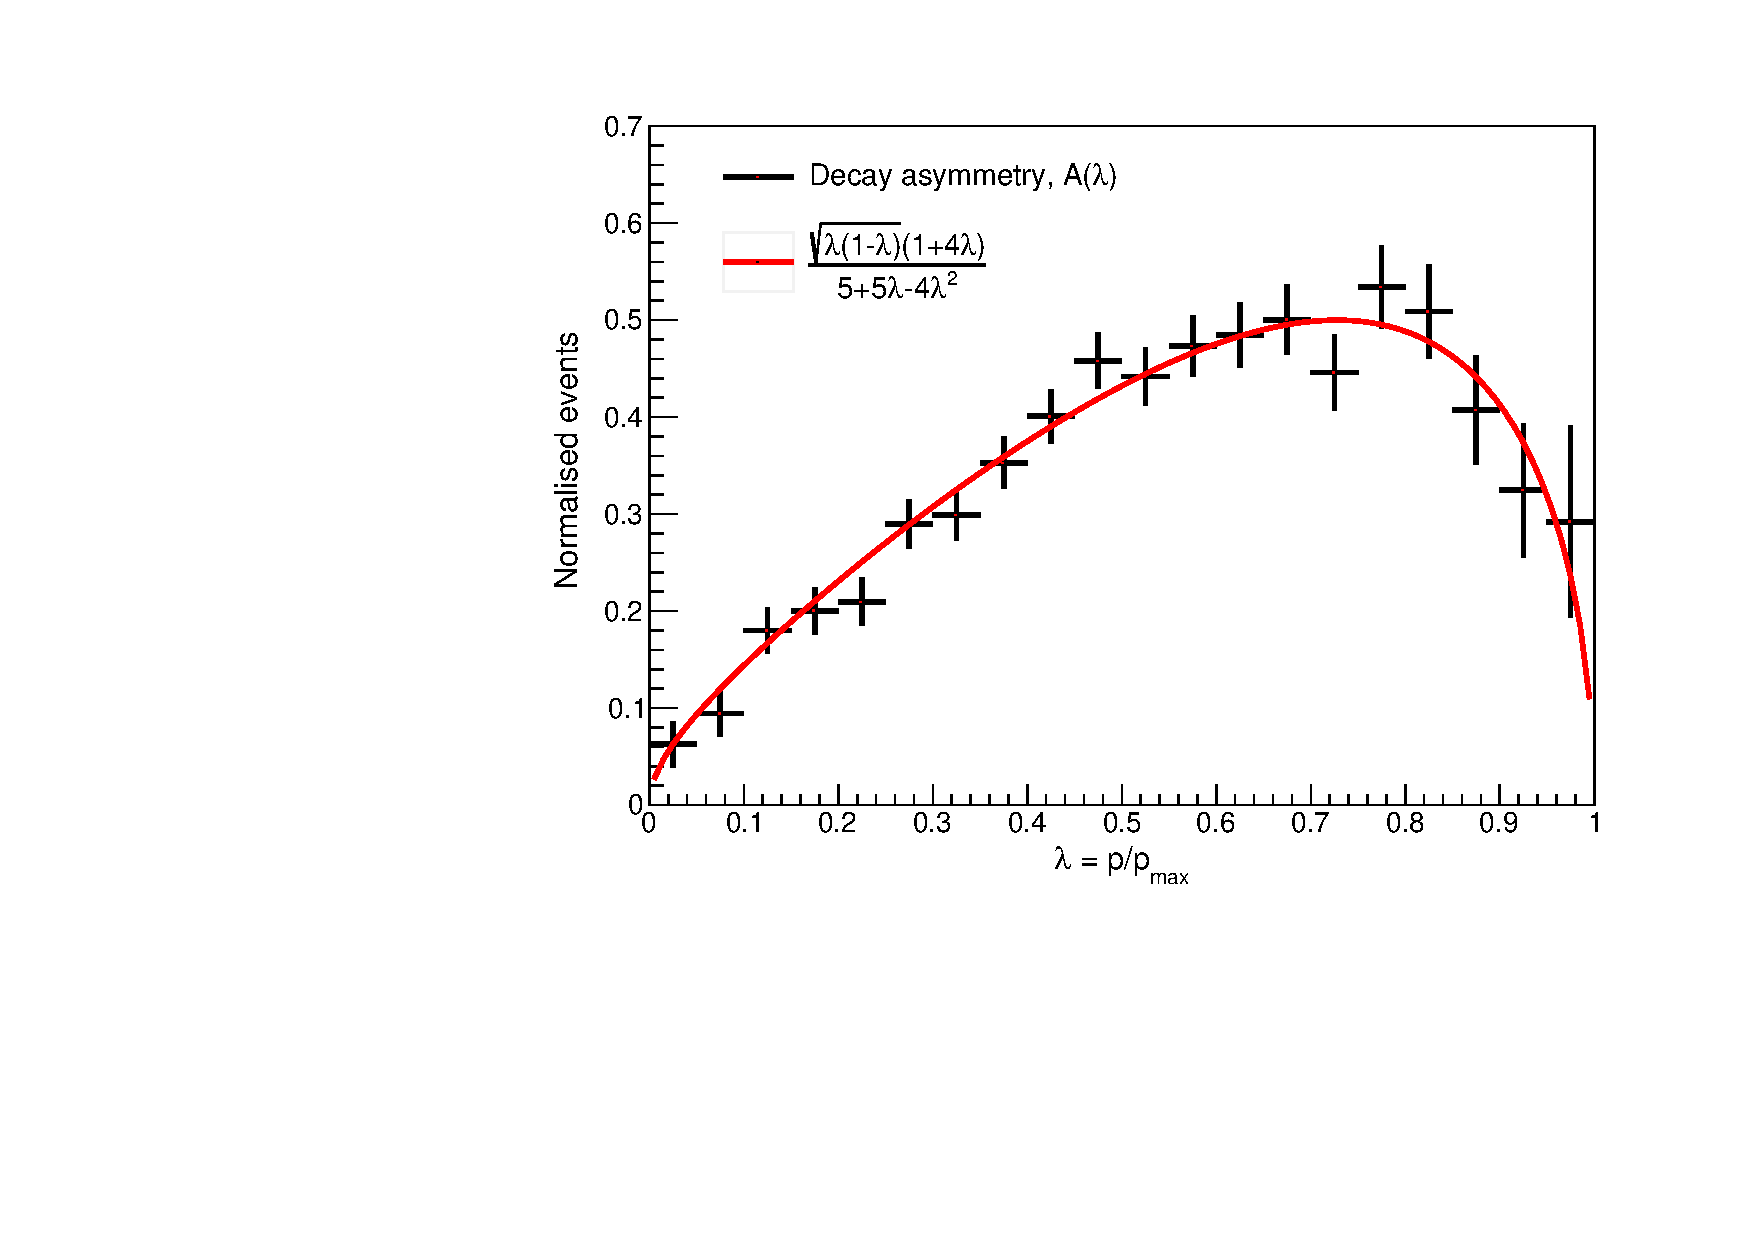
\includegraphics[trim={0 0 0 1cm},clip,width=.49\textwidth]{Images/Chapter5/hFit_A_LAB_TEST.pdf}\label{subfig:SimEDMAsymFit}}
\caption{EDM decay asymmetry verification, showing: (a) The simulated distributions of the number function, $N(\lambda)$, the decay asymmetry function, $A(\lambda)$, and the statistical FOM function, $NA^{2}(\lambda)$, in the laboratory frame; (b) the analytical form of $A(\lambda)$ overlaid on the corresponding simulated distribution, showing excellent agreement.}
\label{fig:SimAsymmetry_EDM}
\end{figure} 

\section{Fitting the vertical angle oscillation}\label{sec:FittingThetaYSim}

As introduced in Chapter \ref{chap:2} Section \ref{subsec:VerticalAngleBasedSearch}, the measured signal in this analysis is the vertical angle in-phase with the EDM oscillation, $A_{\text{EDM}}$. This quantity may be accessed by fitting for an oscillation in the average vertical angle as a function of time, $\langle \theta_{y} \rangle(t)$, which is phase shifted by $\pi/2$ from the anomalous precession oscillation (the number oscillation, introduced in Chapter \ref{chap:2} Section \ref{subsec:SensitivityToOmegaA}). Therefore, the first step in the analysis is to fit the number oscillation for the anomalous precession oscillation phase, $\phi$, using the five parameter function given by Equation \ref{eqn:FiveParFunc}. $\langle \theta_{y} \rangle(t)$ may then be fitted with Equation \ref{eqn:VertAngleFitFunc} for $A_{\text{EDM}}$, with $\phi$ as a fixed parameter. $\omega_{a}$ is fixed to a value of 1.439311 rad$/$\SI{}{\micro\second} throughout, which is the average measured value for the positive muon at the BNL $g-2$ experiment \cite{BNLFinalReport}.

Furthermore, the muon EDM search presented in this thesis employs momentum-binned approach, which is motivated, in part, by the momentum dependence of $A_{\text{EDM}}$ -- or, the momentum dependence of the total dilution of $\delta$ -- described by Equation \ref{eqn:DilutionFunction2}. Additionally, and as will be discussed in both Section \ref{sec:AvgVertAngleSim} and Chapter \ref{chap:6} Section \ref{subsec:AvgVertAngleData}, the average vertical angle itself possesses a momentum dependence (due to acceptance effects), further motivating a momentum-binned analysis. Fits to the vertical angle oscillation without the use of this technique, where momentum intervals are fitted simultaneously, are referred to in this thesis as `simultaneous fits'. These are performed as a cross-check of the main results. 

% This approach is designed to increase sensitivity,  in order to 

% The aforementioned dependence of the average vertical angle on momentum, along with the fact that $A_{\text{EDM}}$ is itself momentum dependent by Equation \ref{eqn:DilutionFunction} -- or, more specifically, the level to which $\delta$ is diluted, $d_{\text{EDM}}$, is momentum dependent -- motivates an analysis which is conducted in momentum intervals. This approach reduces the variation of the average vertical angle in each fit. Distributions of $A_{\text{EDM}}$ for fits per 250 MeV are shown in Figure \ref{fig:AEDM_overlay_sim}. The impact of tracker acceptance is clear, manifesting as a significant decrease in sensitivity which is most pronounced at low momentum. 

\subsection{Modulation at the anomalous precession period}\label{sec:TimeMod}

\begin{figure}[b!]
\centering{}
\subfloat[Unmodulated.]{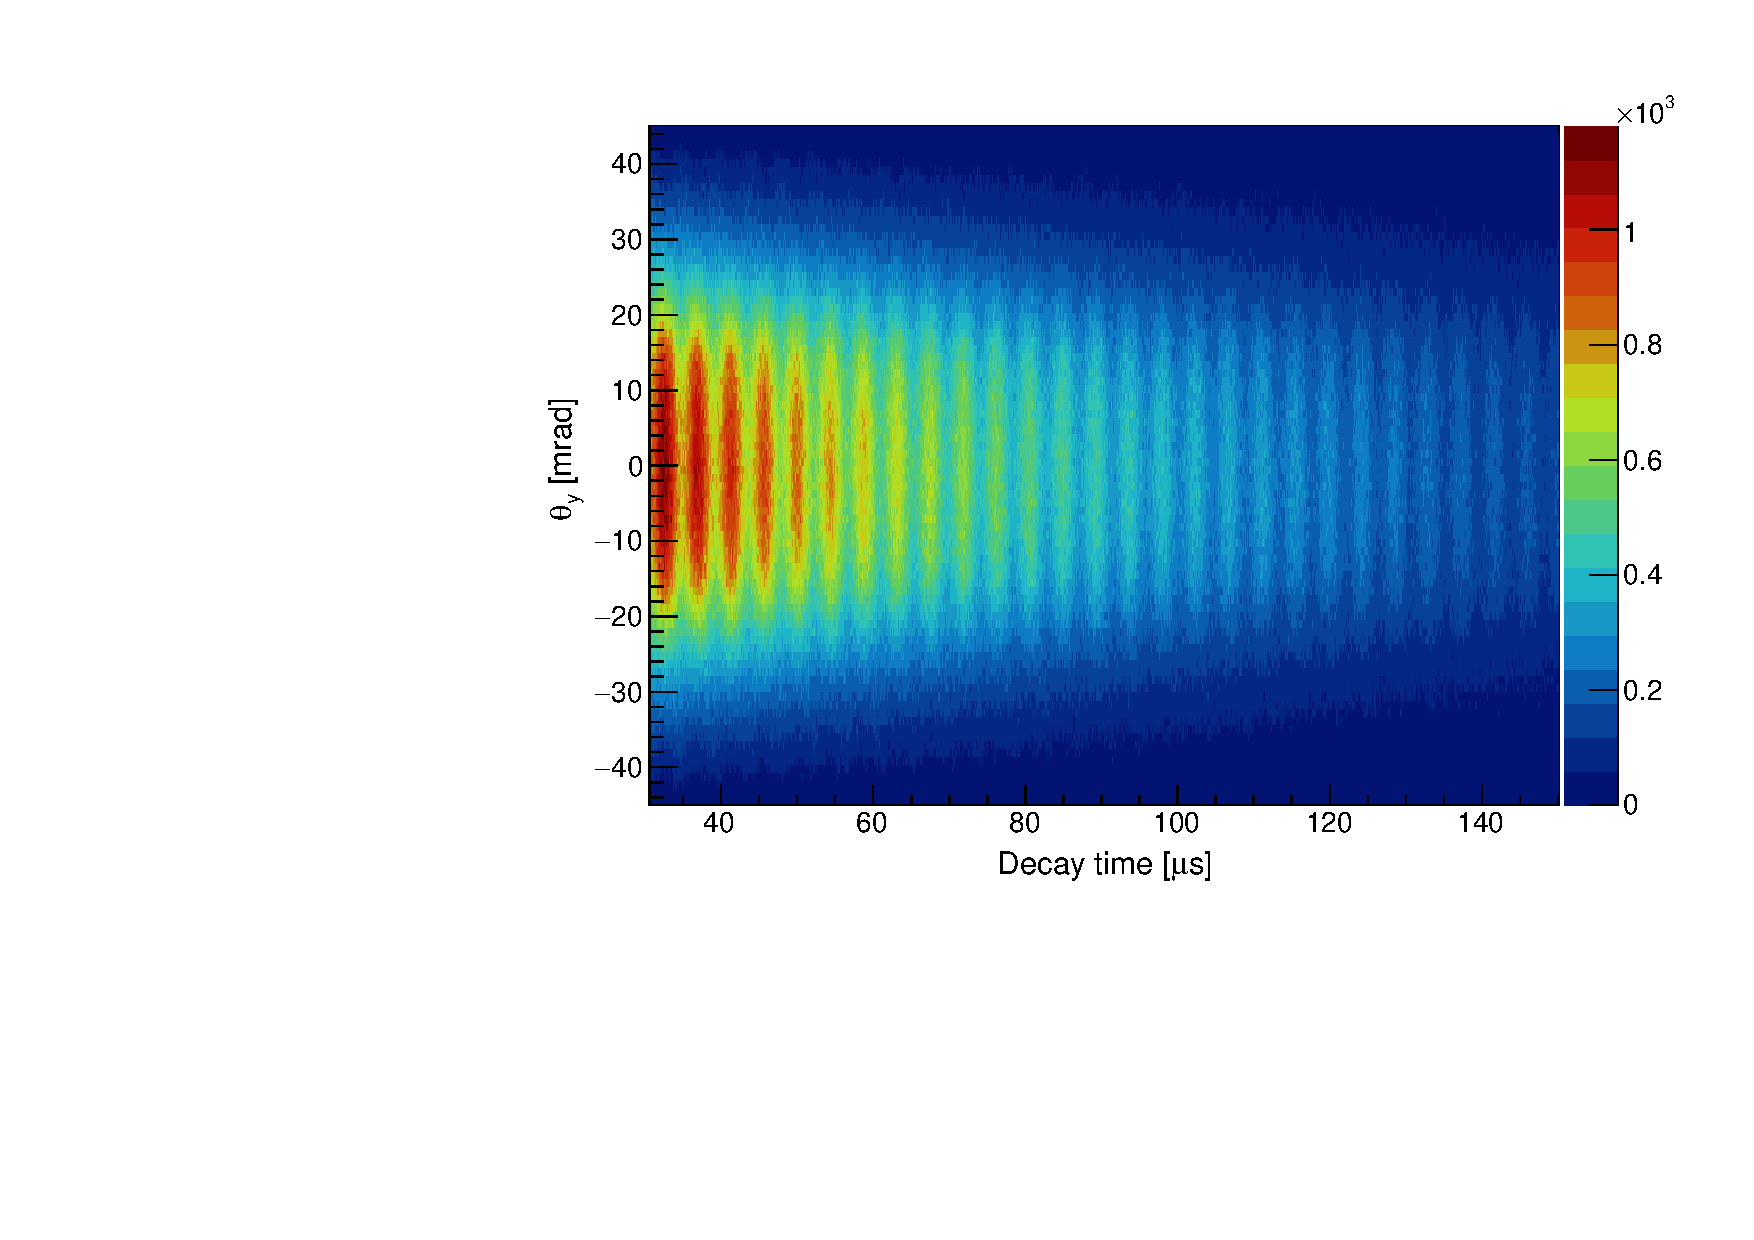
\includegraphics[trim={0 0 0 0},clip,width=.49\textwidth]{Images/Chapter5/allDecays_ThetaY_vs_t.pdf}\label{subfig:Unmodulated}}
\subfloat[Modulated.]{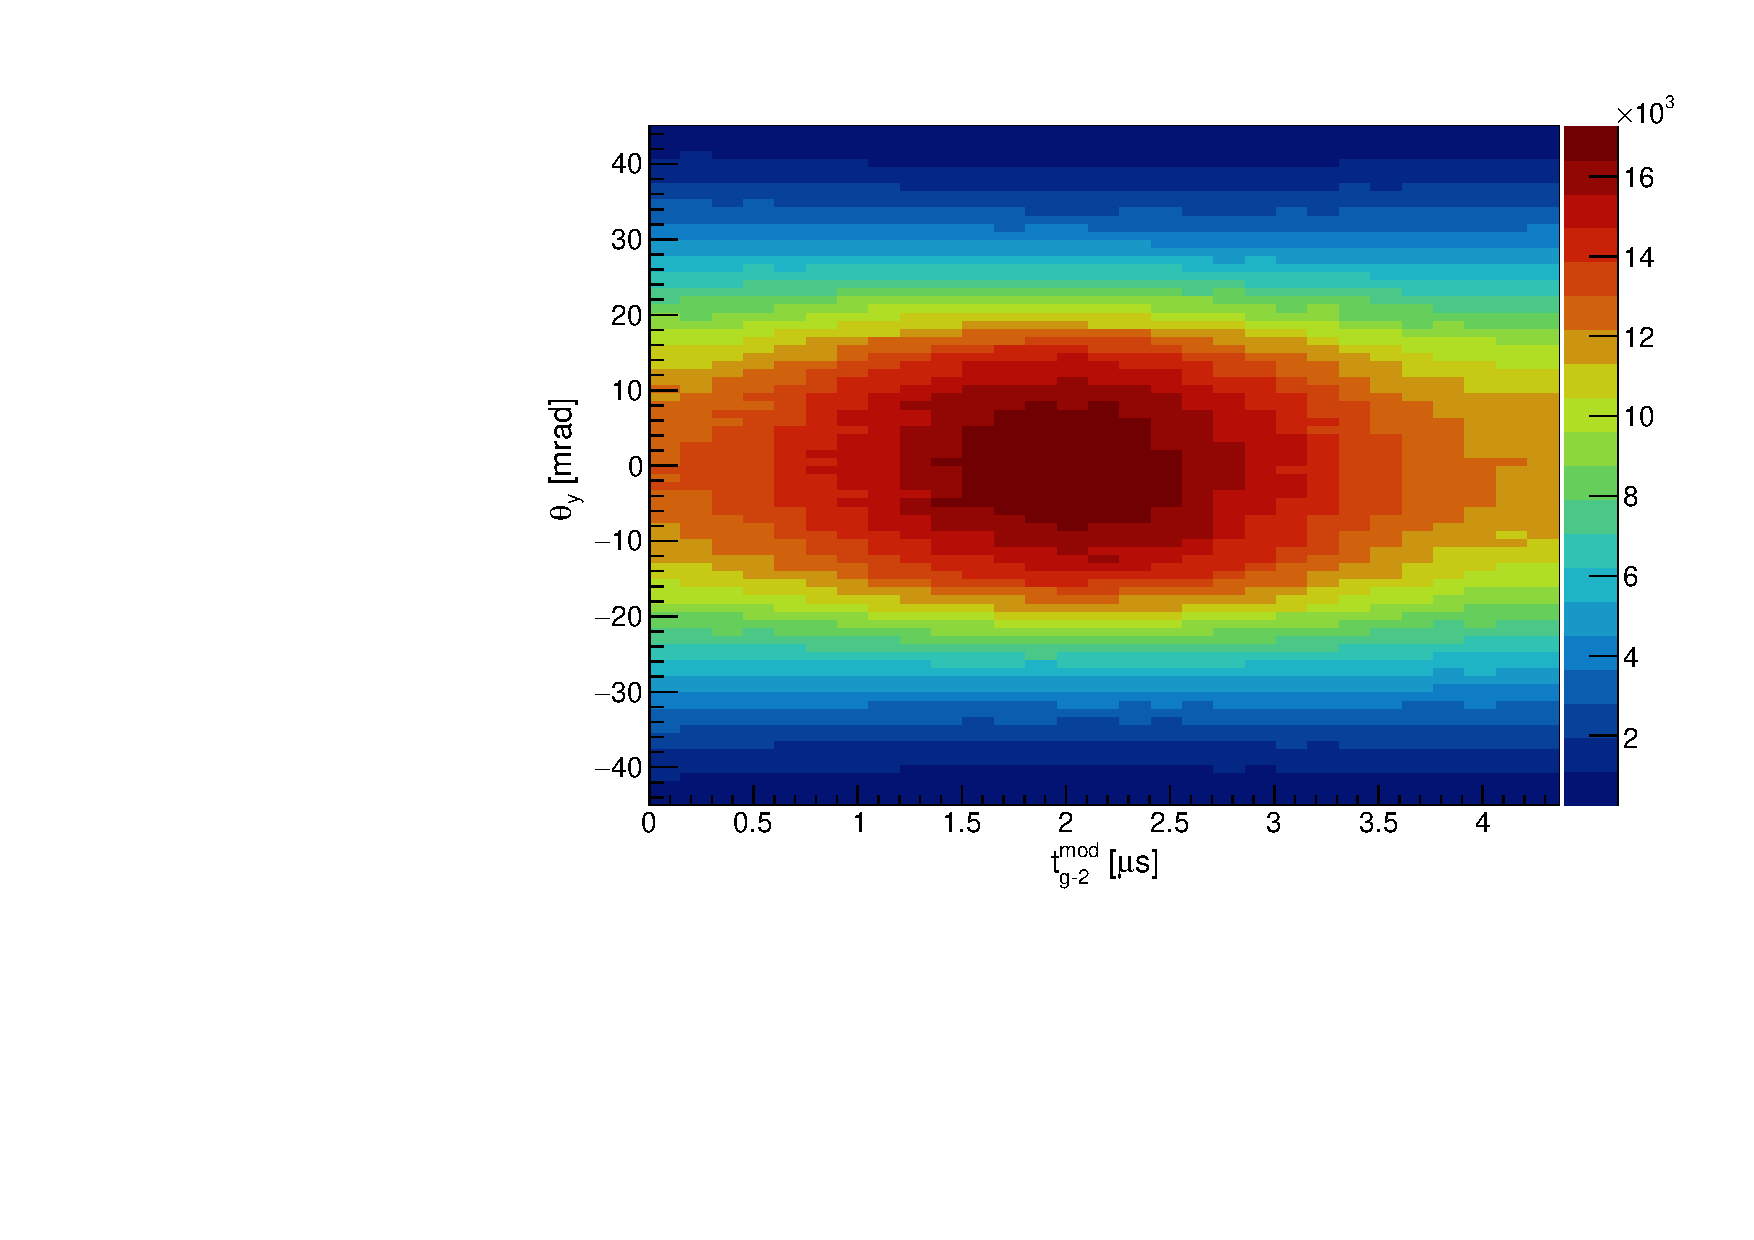
\includegraphics[trim={0 0 0 0},clip,width=.49\textwidth]{Images/Chapter5/allDecays_ThetaY_vs_t_modulo.pdf}\label{subfig:Modulated}}
\caption{The effects of time modulation at the anomalous precession period, showing the distribution of vertical decay angles over time with (a) no modulation, and (b) with modulation. The distributions pictured are formed from the \textit{all decays} reconstruction.}
\label{fig:TimeModulation}
\end{figure}  

In the analysis of both simulation and Run-1 data, which is presented in Chapter \ref{chap:6}, the number oscillation and the vertical angle oscillation are modulated at the anomalous precession period, $T_{g-2} = \text{\SI{4.365}{\micro\second}}$. This simply means that the distribution of $\theta_{y}$ as a function of time is divided into periods of $T_{g-2}$, which are then recombined into a single distribution, as demonstrated in Figure \ref{fig:TimeModulation}. Time modulation is employed so as to minimise the influence of oscillations such as the CBO, introduced in Chapter \ref{chap:3} Section \ref{subsec:CBO}, which will de-phase and destructively interfere over many modulated periods. This technique also maximises sensitivity to oscillations with a period equal to $T_{g-2}$, which combine constructively. The modulated time, $t_{g-2}^\text{mod}$, is calculated by 
%
\begin{equation}
  t_{g-2}^{\text{mod}} = \left(\frac{t}{T_{g-2}}-\text{int}\left[\frac{t}{T_{g-2}}\right]\right)\cdot T_{g-2},
  \label{eqn:TimeMod}
\end{equation}
%
which is reproduced from \cite{Lukicov}.

\subsection{Momentum selection}\label{subsec:MomSelect}

\begin{figure}[b!]
\centering{}
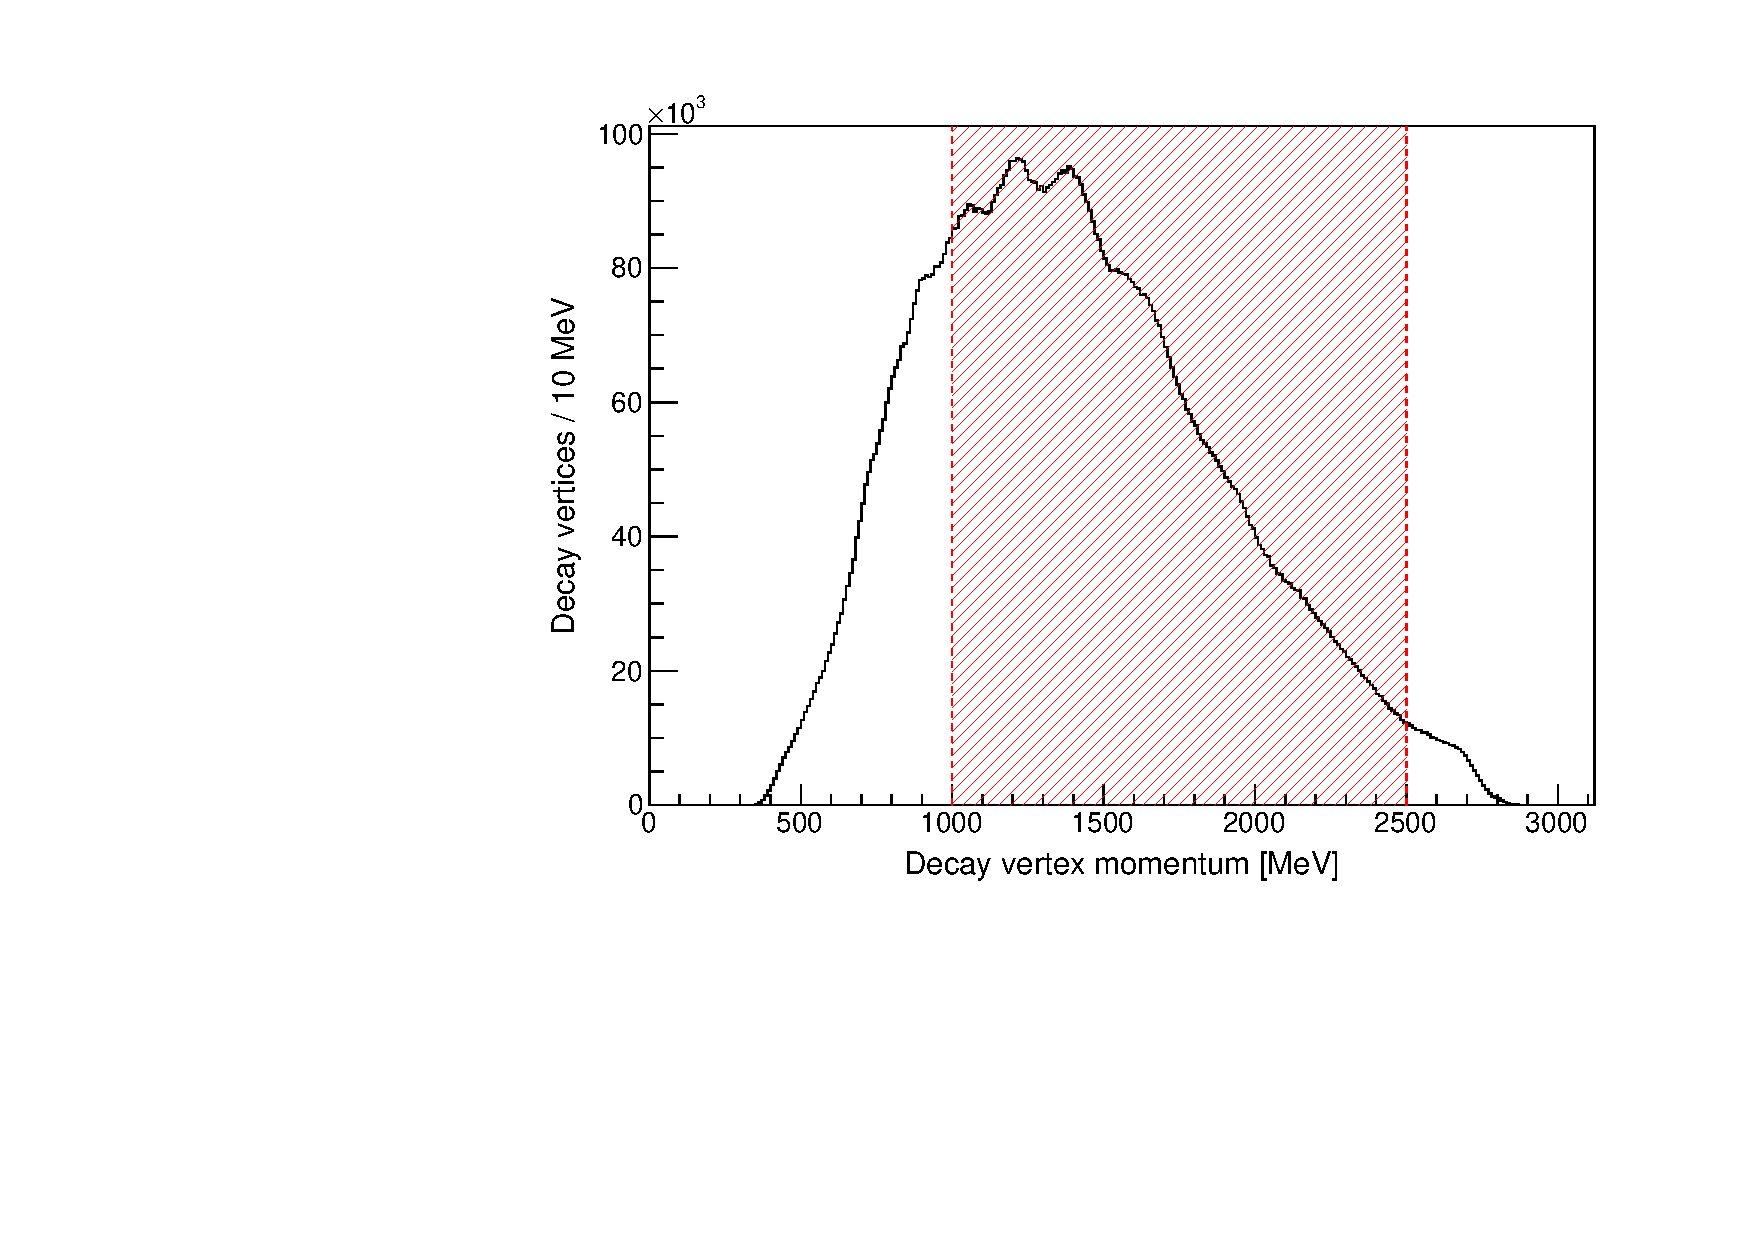
\includegraphics[trim={0 0 0 0},clip,width=.69\textwidth]{Images/Chapter5/RecoMomentum_Simultaneous.pdf}
\caption{The positron momentum distribution as measured by the straw trackers in Run-1a, illustrating the momentum range selected for the analysis of the vertical angle oscillation. Tracker stations 12 and 18 are combined.}
\label{fig:RecoMomentum_Simultaneous}
\end{figure}  

The maximum statistical sensitivity to a muon EDM occurs at middling decay positron energy, as demonstrated by the statistical FOM function, $NA^{2}(\lambda)$, in Figure \ref{fig:Asymmetry_EDM}. Consequently, cuts are imposed to select tracks of middling momentum. The choice of momentum range also depends on the momentum acceptance of the trackers, which drops off sharply below 1000 MeV. Accounting for this, the momentum range was chosen to be 1000-2500 MeV: a region overlaid on the momentum distribution as measured by the straw trackers in Run-1a in Figure \ref{fig:RecoMomentum_Simultaneous}. In the case of the anomalous precession oscillation, a low energy threshold of 1.7 GeV was used, based on the optimum threshold for maximising the statistical sensitivity to the anomalous precession oscillation, discussed in Chapter \ref{chap:2} Section \ref{subsec:SensitivityToOmegaA}.

\subsection{Anomalous precession oscillation fits}

Fits to the number oscillation for the anomalous precession oscillation phase, $\phi$, for each of the three reconstructions of the 30$\times$ BNL Monte Carlo sample, are shown in Figures \ref{subfig:AllDecaysWiggle}, \ref{subfig:TruthWiggle}, and \ref{subfig:RecoWiggle}. The measured phases are included in Table \ref{tbl:BasicSimFits}.

An early time cut of \SI{30.6}{\micro\second}, or seven multiples of $T_{g-2}$\footnote{When utilising time modulation, time cuts must be placed at a multiple of the modulation period.}, is imposed. This time cut is essential to avoid ESQ scraping, as well as the worst effects of the fast rotation and muon losses (described in Chapter \ref{chap:3}). In order to remove any residual fast rotation effects, the oscillation is binned in time at the cyclotron period, $T_{c} = $\SI{149.2}{\nano\second}, and decay times are uniformly randomised by $\pm T_{c}/2$ about the measured value. Tracker stations 12 and 18 are combined, and station 0 is excluded. 

\afterpage{
\begin{figure}[]
\centering{}
\subfloat[\textit{All decays}: fit for $\phi$.]{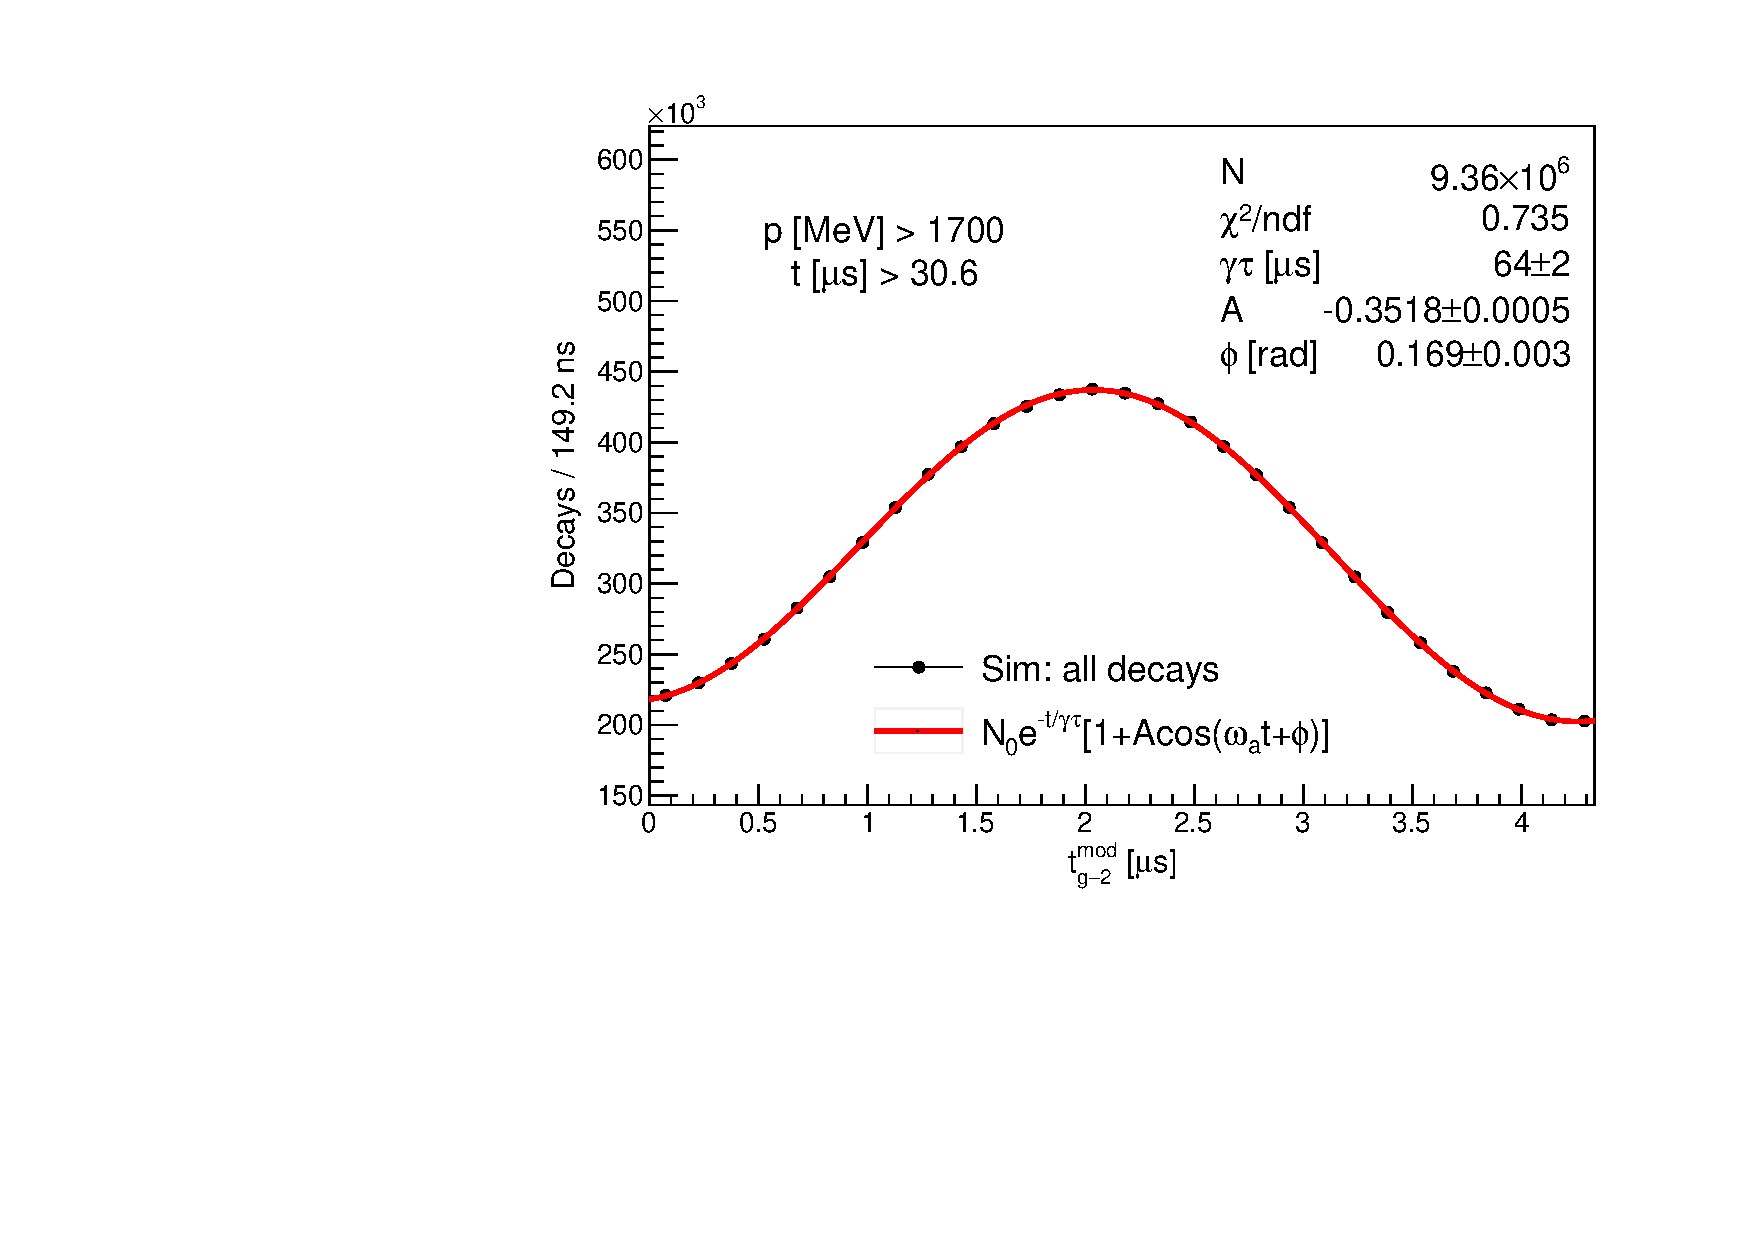
\includegraphics[trim={0 0 0 1cm},clip,width=.49\textwidth]{Images/Chapter5/fit_mod_wiggle_allDecays_WORLD_250MeV_AQ_noVertCorr.pdf}\label{subfig:AllDecaysWiggle}}
\subfloat[\textit{All decays}: fit for $A_\text{EDM}$.]{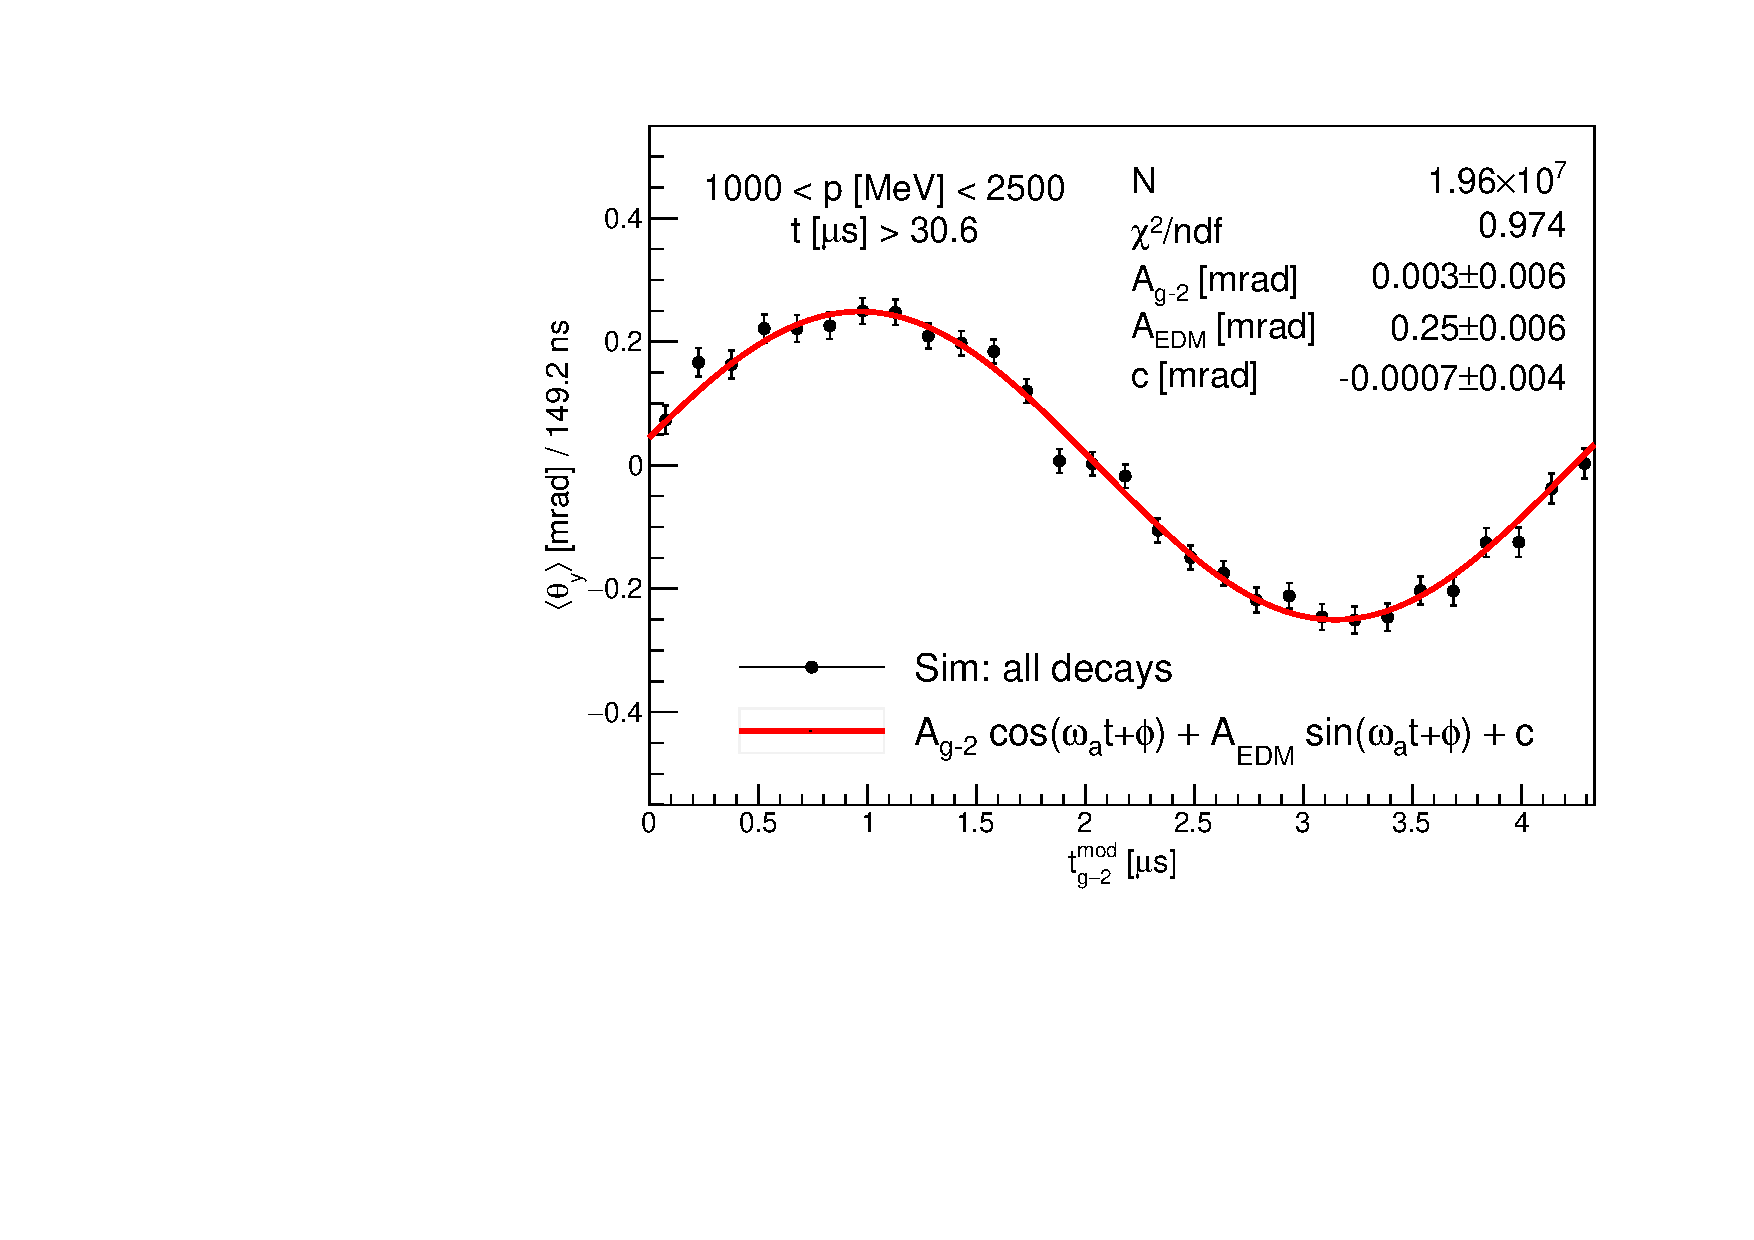
\includegraphics[trim={0 0 0 1cm},clip,width=.49\textwidth]{Images/Chapter5/edmFit_thetaY_allDecays_WORLD_250MeV_AQ_noVertCorr_1.pdf}\label{subfig:AllDecaysBasicFitSim}}
\hfill
\subfloat[\textit{Truth vertices}: fit for $\phi$.]{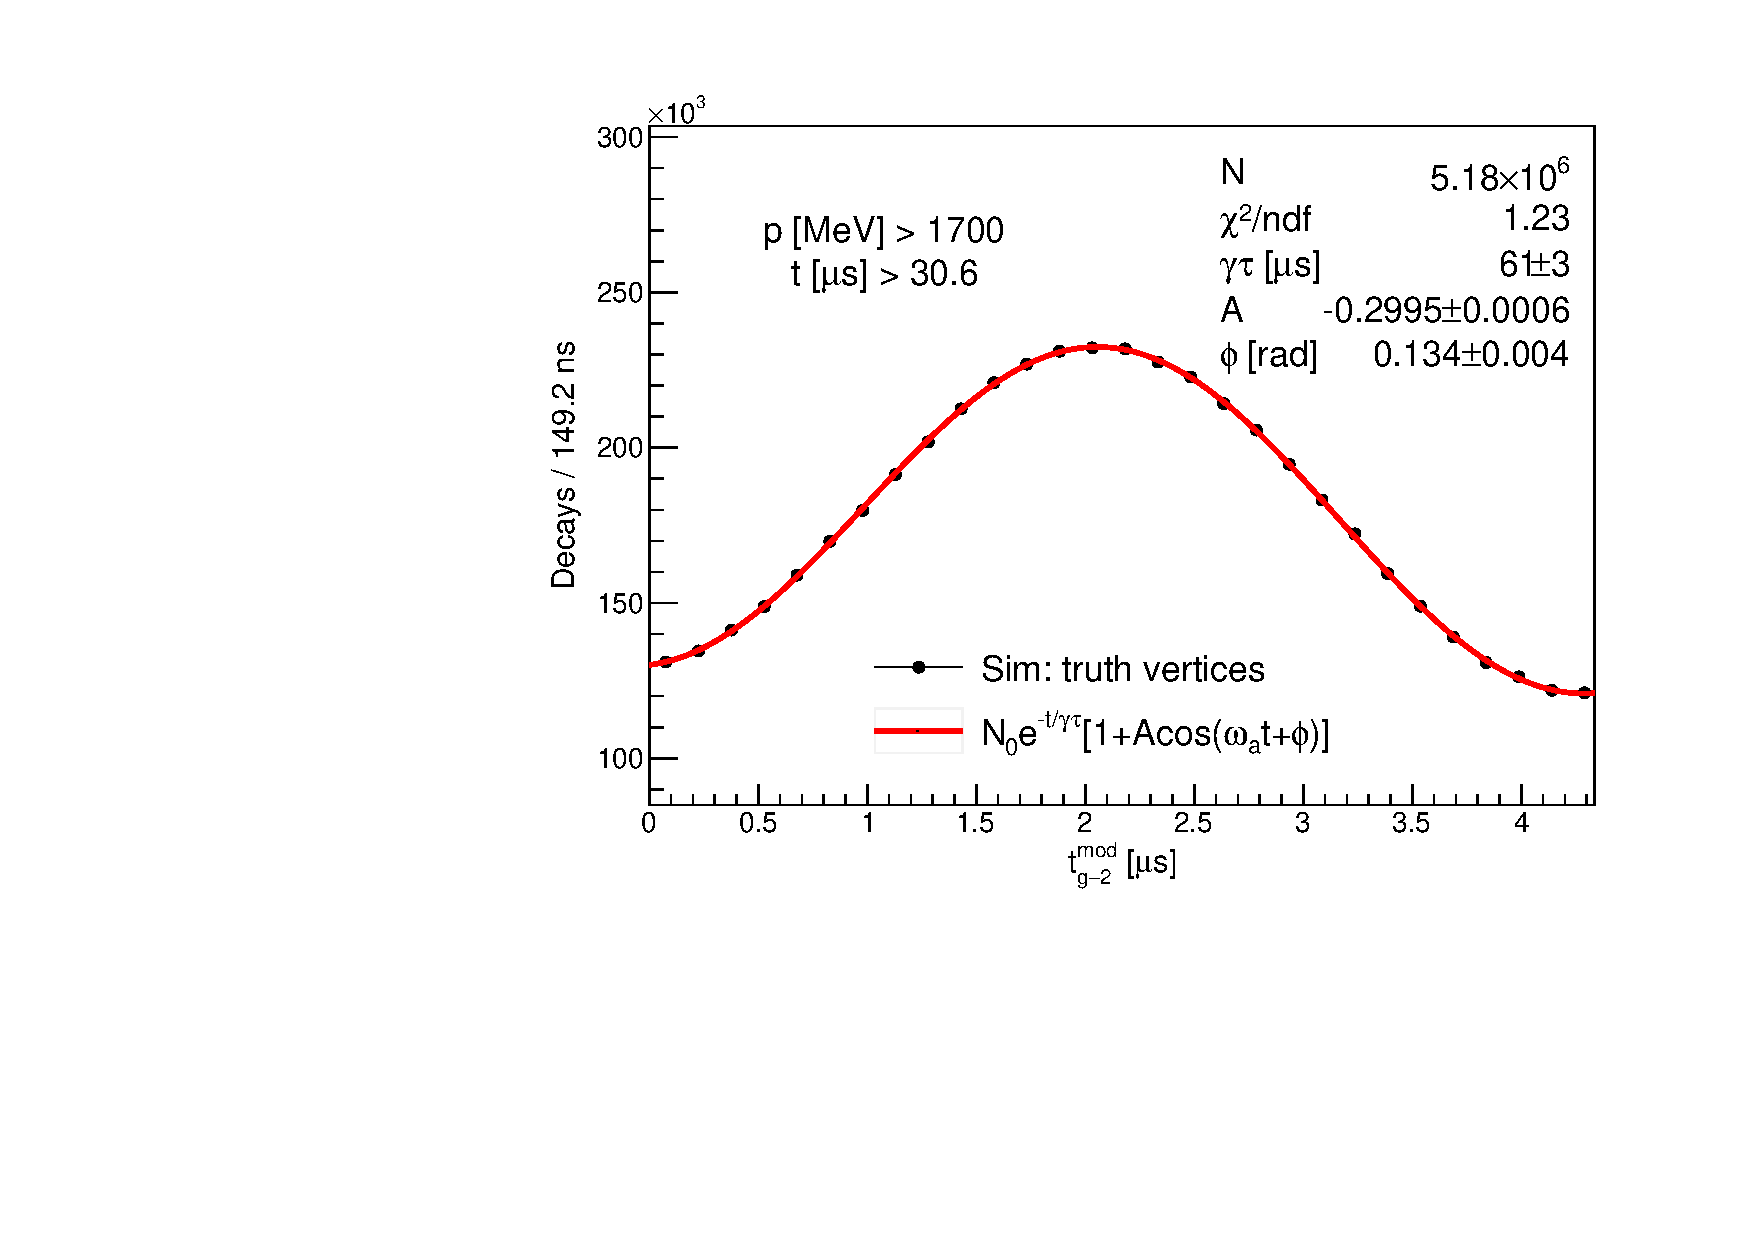
\includegraphics[trim={0 0 0 1cm},clip,width=.49\textwidth]{Images/Chapter5/fit_mod_wiggle_trackTruth_WORLD_250MeV_BQ_noVertCorr.pdf}\label{subfig:TruthWiggle}}
\subfloat[\textit{Truth vertices}: fit for $A_\text{EDM}$.]{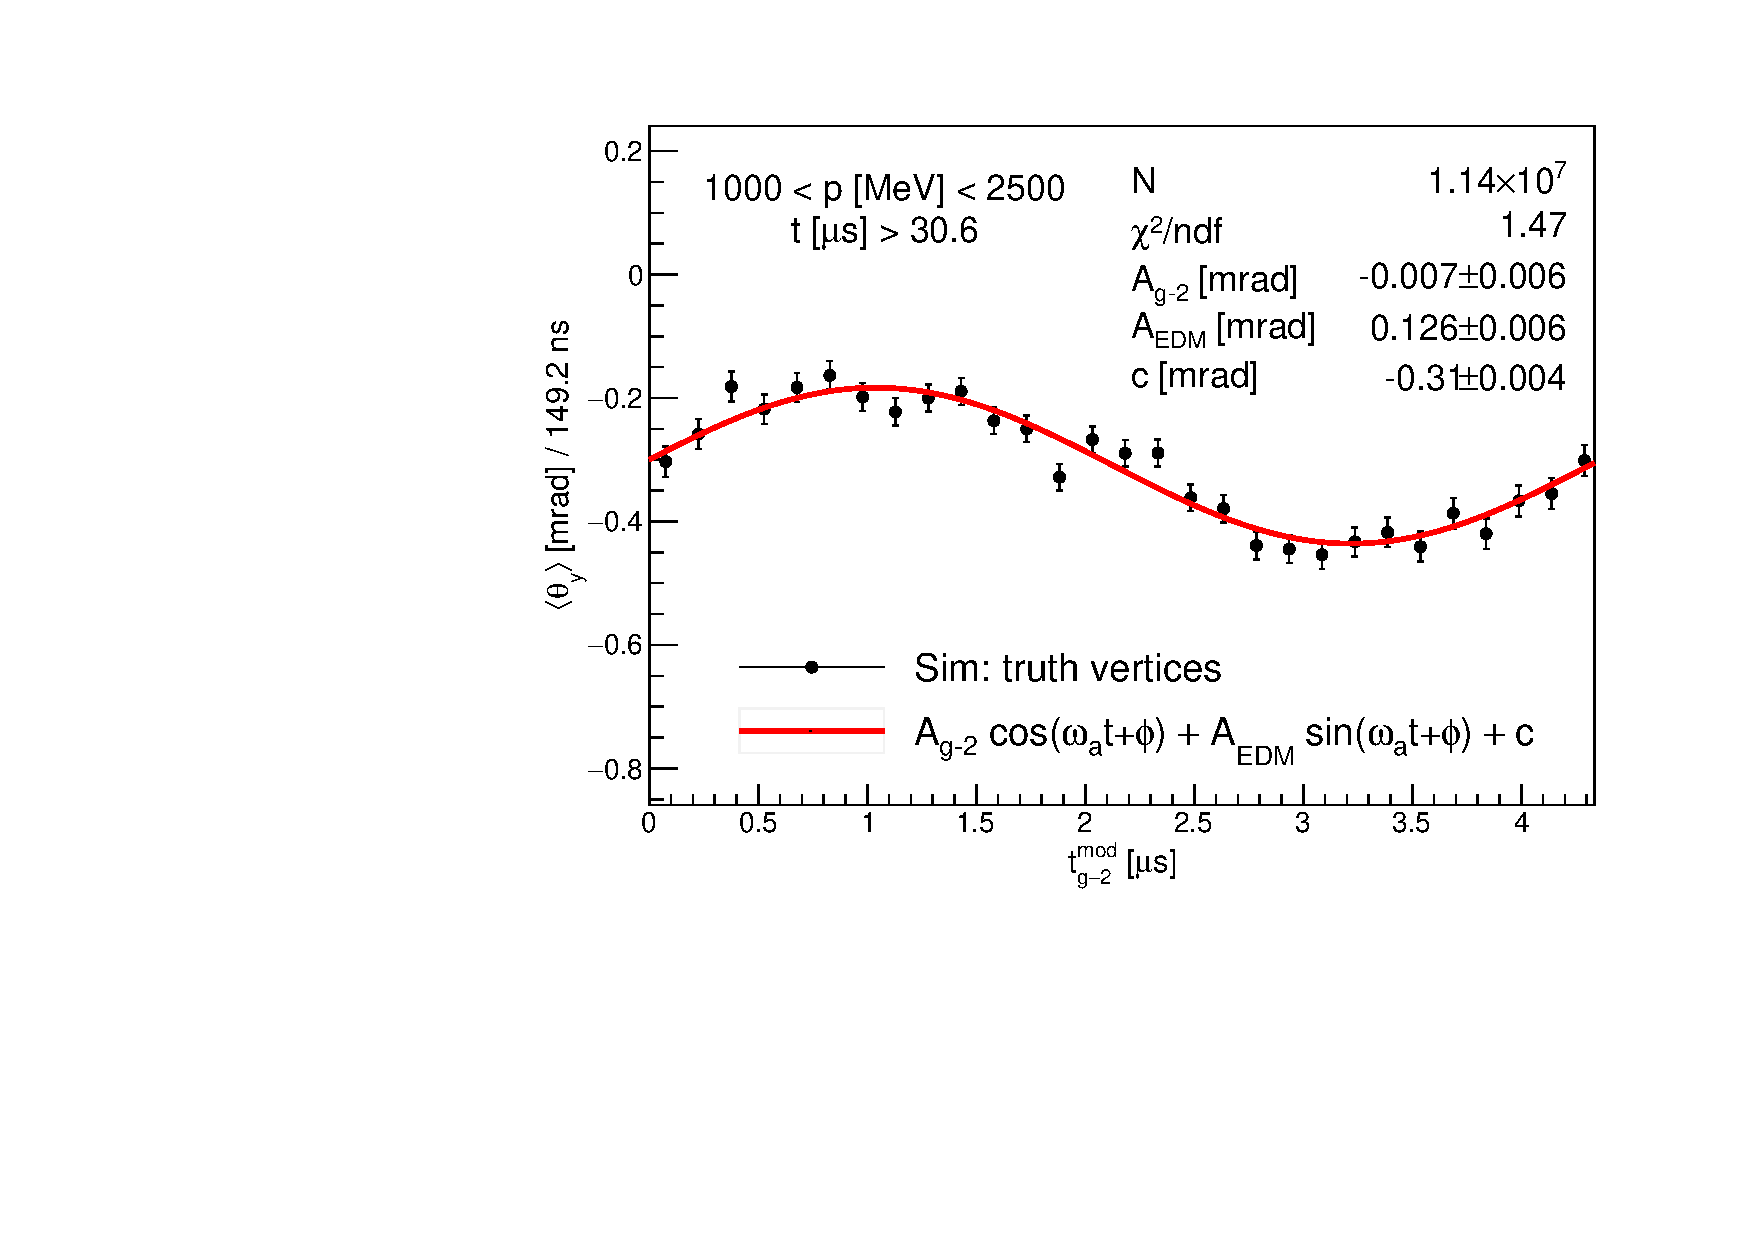
\includegraphics[trim={0 0 0 1cm},clip,width=.49\textwidth]{Images/Chapter5/S12S18_edmFit_thetaY_trackTruth_WORLD_250MeV_BQ_noVertCorr_1.pdf}\label{subfig:TruthBasicFitSim}}
\hfill
\subfloat[\textit{Reco vertices}: fit for $\phi$.]{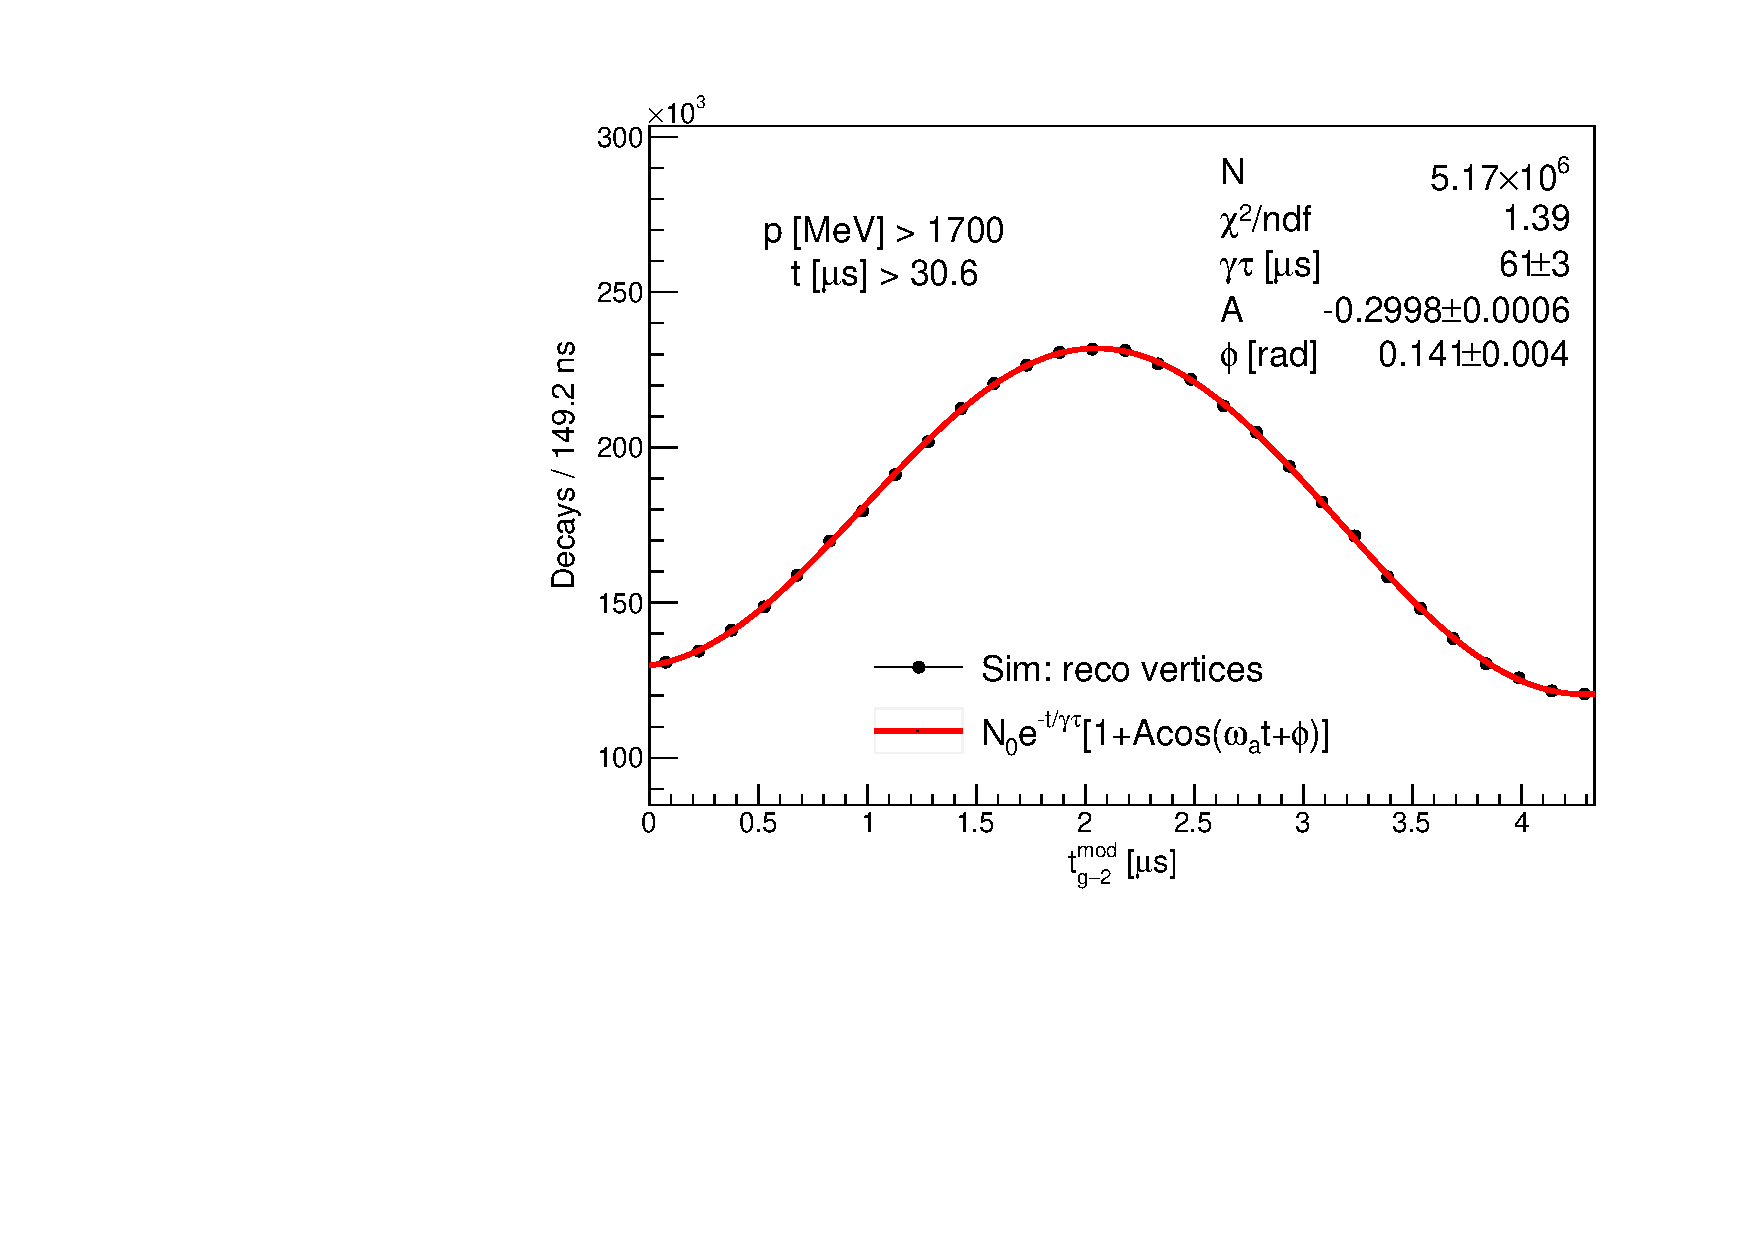
\includegraphics[trim={0 0 0 1cm},clip,width=.49\textwidth]{Images/Chapter5/fit_mod_wiggle_trackReco_WORLD_250MeV_BQ_noVertCorr.pdf}\label{subfig:RecoWiggle}}
\subfloat[\textit{Reco vertices}: fit for $A_\text{EDM}$.]{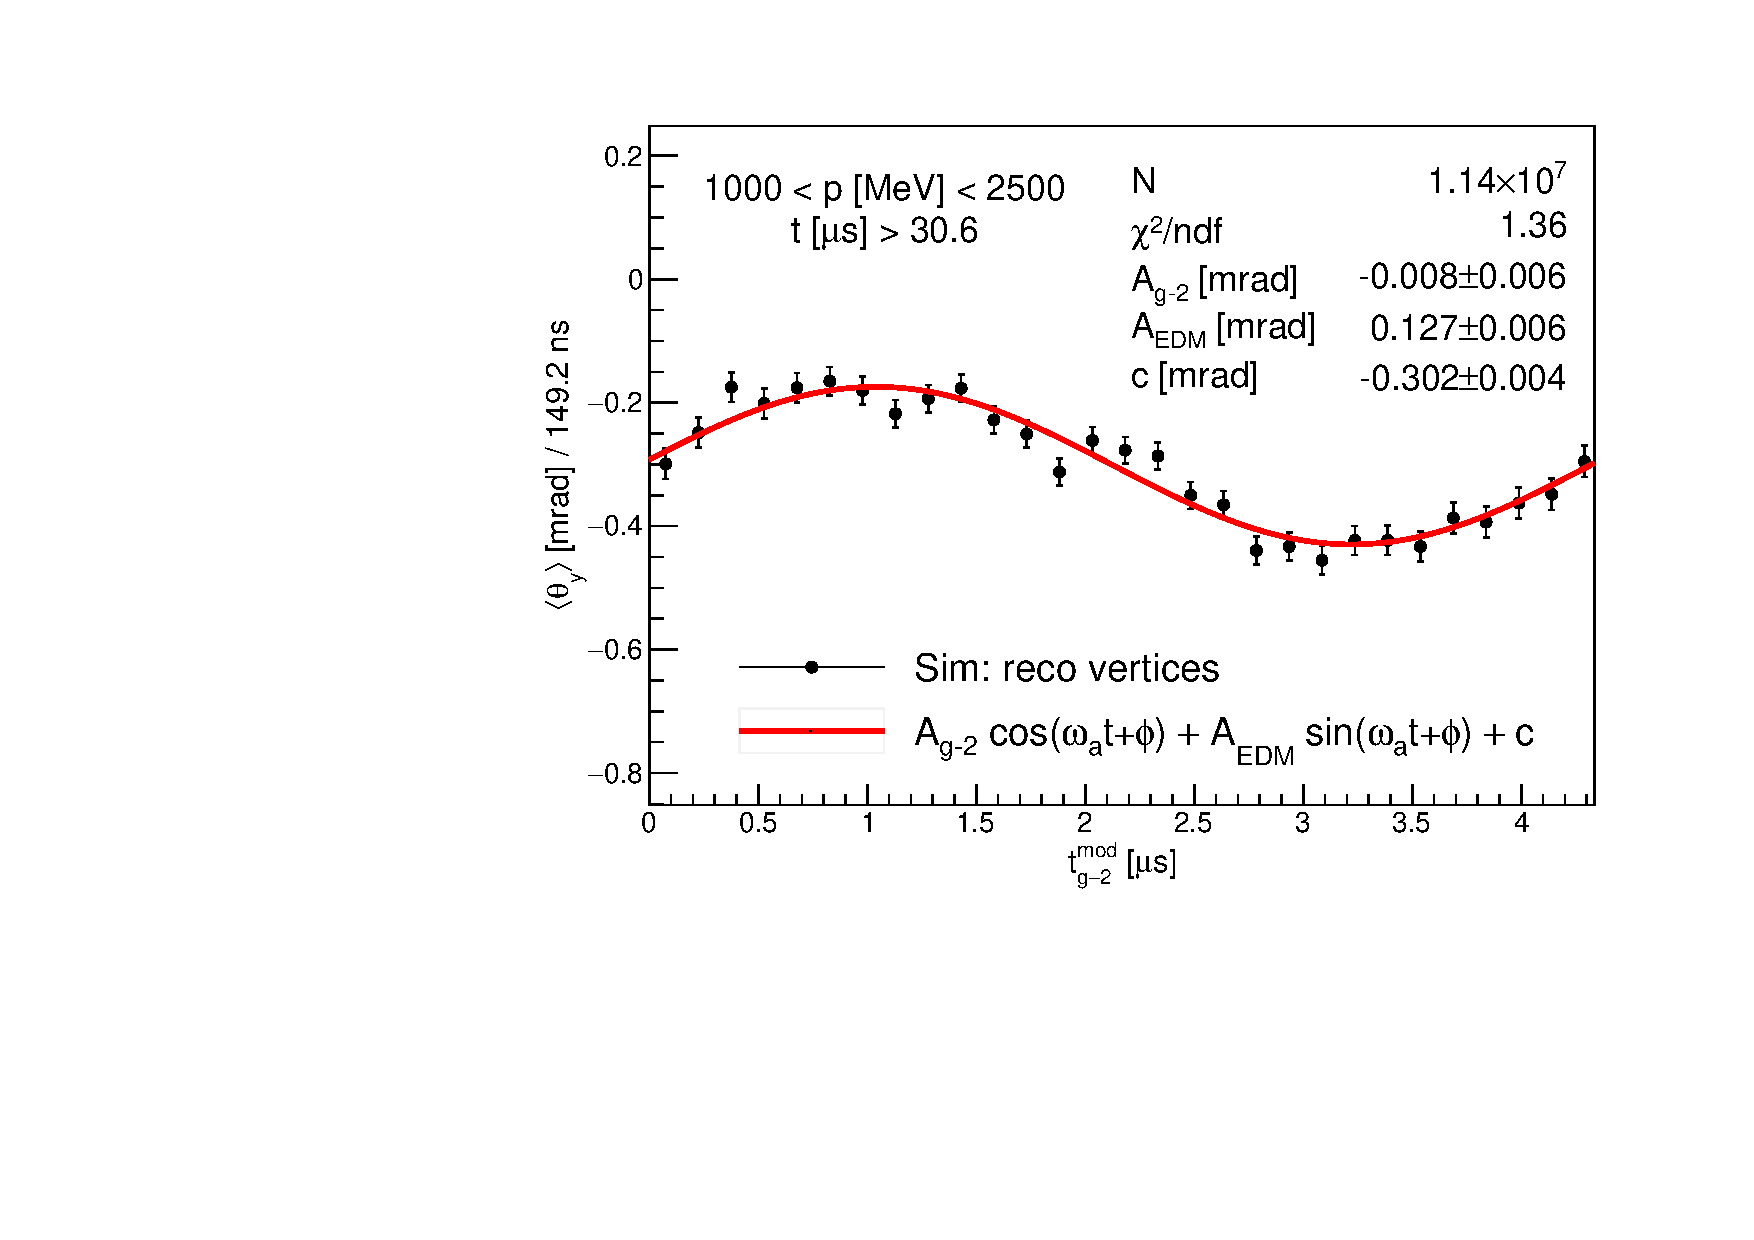
\includegraphics[trim={0 0 0 1cm},clip,width=.49\textwidth]{Images/Chapter5/S12S18_edmFit_thetaY_trackReco_WORLD_250MeV_BQ_noVertCorr_1.pdf}\label{subfig:RecoBasicFitSim}}
\caption{Fits to both the number oscillation, for the anomalous precession phase $\phi$, and the average vertical angle oscillation, for the observed EDM vertical angle, $A_{\text{EDM}}$. Tracker stations 12 and 18 are combined, and station 0 is excluded. As discussed in the text, the inclusion of detector acceptance results in a more pronounced dilution of the tilt angle, $\delta = 1.69$ mrad. $A_{\text{EDM}}$ is consistent between \textit{truth vertices} and \textit{reco vertices}.}
\label{fig:BasicSimFits}
\end{figure}
\clearpage
} 

\subsection{Simultaneous vertical angle oscillation fits}\label{subsec:BasicVertAngFitsSim}

\begin{table}[b!]
\centering{}
\begin{tabular}{l|cccc}
\hline
\hline
Label & $\chi^{2}/\text{NDF}$ & $\phi$ [rad] & $A_{\text{EDM}}$ [mrad] & $d_{\text{EDM}}$ \\
\hline
\textit{All decays}     & $0.974$ & $0.169\pm0.003$ & $0.250\pm0.006$ & $0.148\pm0.004$ \\
\textit{Truth vertices} & $1.47$  & $0.134\pm0.004$ & $0.126\pm0.006$ & $0.075\pm0.004$ \\
\textit{Reco vertices}  & $1.36$  & $0.141\pm0.004$ & $0.127\pm0.006$ & $0.075\pm0.004$ \\
\hline
\hline
\end{tabular}
\caption{A summary of fit results, corresponding to Figure \ref{fig:BasicSimFits}, listing: the $\chi^{2}/\text{NDF}$, the observed $A_{\text{EDM}}$, and the dilution, $d_{\text{EDM}}$, for each reconstruction. The results of the vertical angle oscillation fits are consistent between \textit{truth vertices} and \textit{reco vertices}, and the \textit{all decays} sample demonstrates the greatest sensitivity to the injected EDM.} 
\label{tbl:BasicSimFits}
\end{table}

Fits to the average vertical angle oscillation over the momentum range of 1000-2500 MeV, for $A_{\text{EDM}}$, are shown in Figures \ref{subfig:AllDecaysBasicFitSim}, \ref{subfig:TruthBasicFitSim}, and \ref{subfig:RecoBasicFitSim}, for each of the three reconstructions of the 30$\times$ BNL Monte Carlo sample. For the same reasons as given in the context of the anomalous precession oscillation fits, an early time cut of \SI{30.6}{\micro\second} is imposed, and decays times are both measured in intervals of $T_{c}$ and uniformly randomised by $\pm T_{c}/2$ about the measured value. %In data, this time cut is essential to avoid ESQ scraping, as well as the worst effects of the fast rotation and muon losses (described in Chapter \ref{chap:3}).

The reduced $\chi^{2}$ of the vertical angle fits, the observed $A_{\text{EDM}}$, and the average dilution factor in this momentum range are given in Table \ref{tbl:BasicSimFits}. Importantly, these results highlight the impact of detector acceptance, in that the average reduction of $A_{\text{EDM}}$ compared to $\delta$ is more pronounced for \textit{truth/reco vertices} by an approximate factor of two. The fit quality also degrades with the inclusion of acceptance, as seen in the change in $\chi^{2}/\text{NDF}$.

\subsection{The dependence of the average vertical angle on momentum in simulation}\label{sec:AvgVertAngleSim}

For extrapolated track decay vertices, the average vertical angle, $\langle \theta_{y} \rangle$, is offset from zero; as demonstrated by the  parameter $c$ in vertical angle oscillation fits shown in Figure \ref{fig:BasicSimFits}. This offset has a dependence on momentum, which is not observed in the \textit{all decays} reconstruction above 500 MeV, shown by Figure \ref{subfig:VerticalOffsetSimOverlay}. From this, it may be inferred that this momentum dependence is a consequence of detector effects rather than a physical change in the true average vertical angle. Moreover, the fact that the offset is less pronounced in tracker station 0, as shown in Figure \ref{subfig:VerticalOffsetSimStationOverlay}, which has perfect global alignment (expanded upon Section \ref{sec:Alignment}) with the beam in simulation, indicates that this effect is partly related to global tracker alignment, and by extension detector acceptance. This dependence is also present in data, as will be discussed in Chapter \ref{chap:6} Section \ref{subsec:AvgVertAngleData}.

\begin{figure}[b!]
\centering{}
\subfloat[]{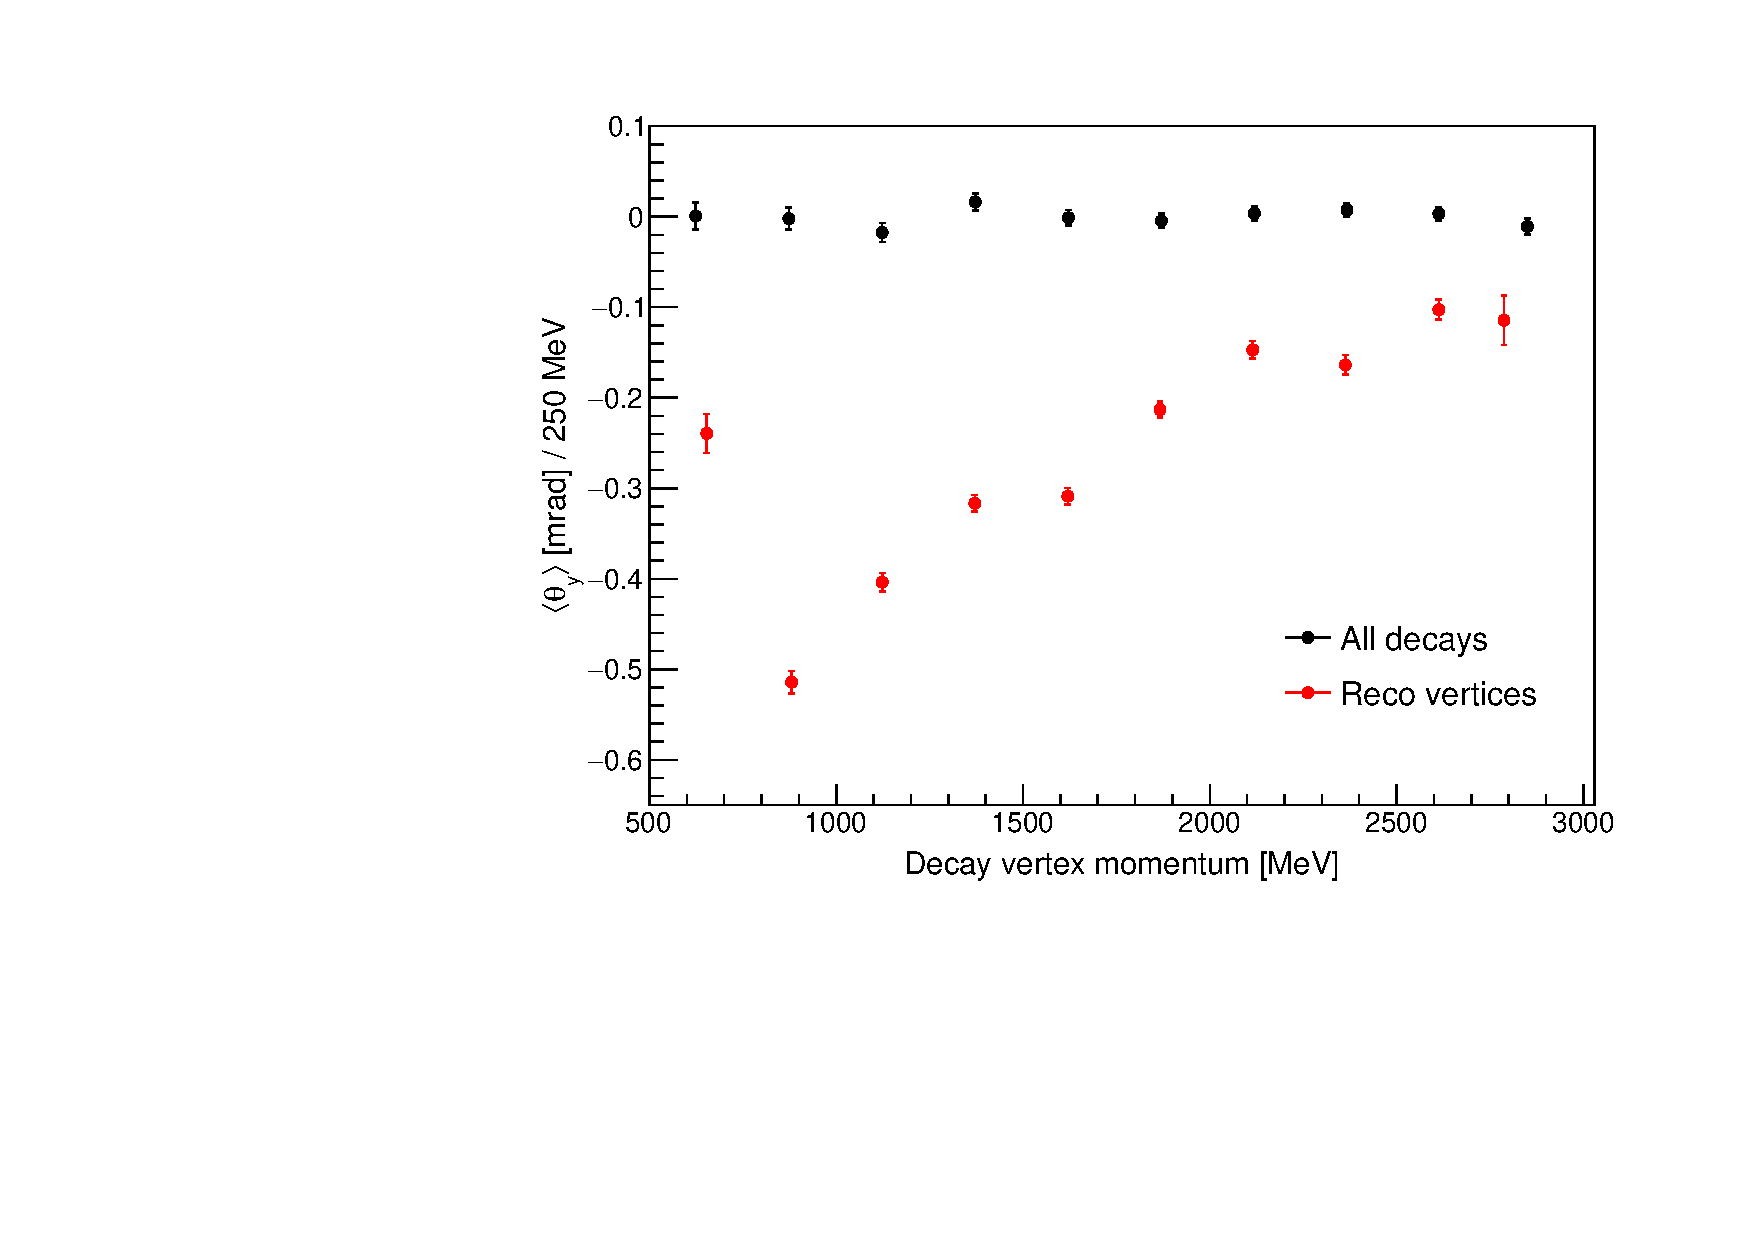
\includegraphics[trim={0 0 0 0},clip,width=.49\textwidth]{Images/Chapter5/VerticalOffsetSimOverlay.pdf}\label{subfig:VerticalOffsetSimOverlay}}
\subfloat[]{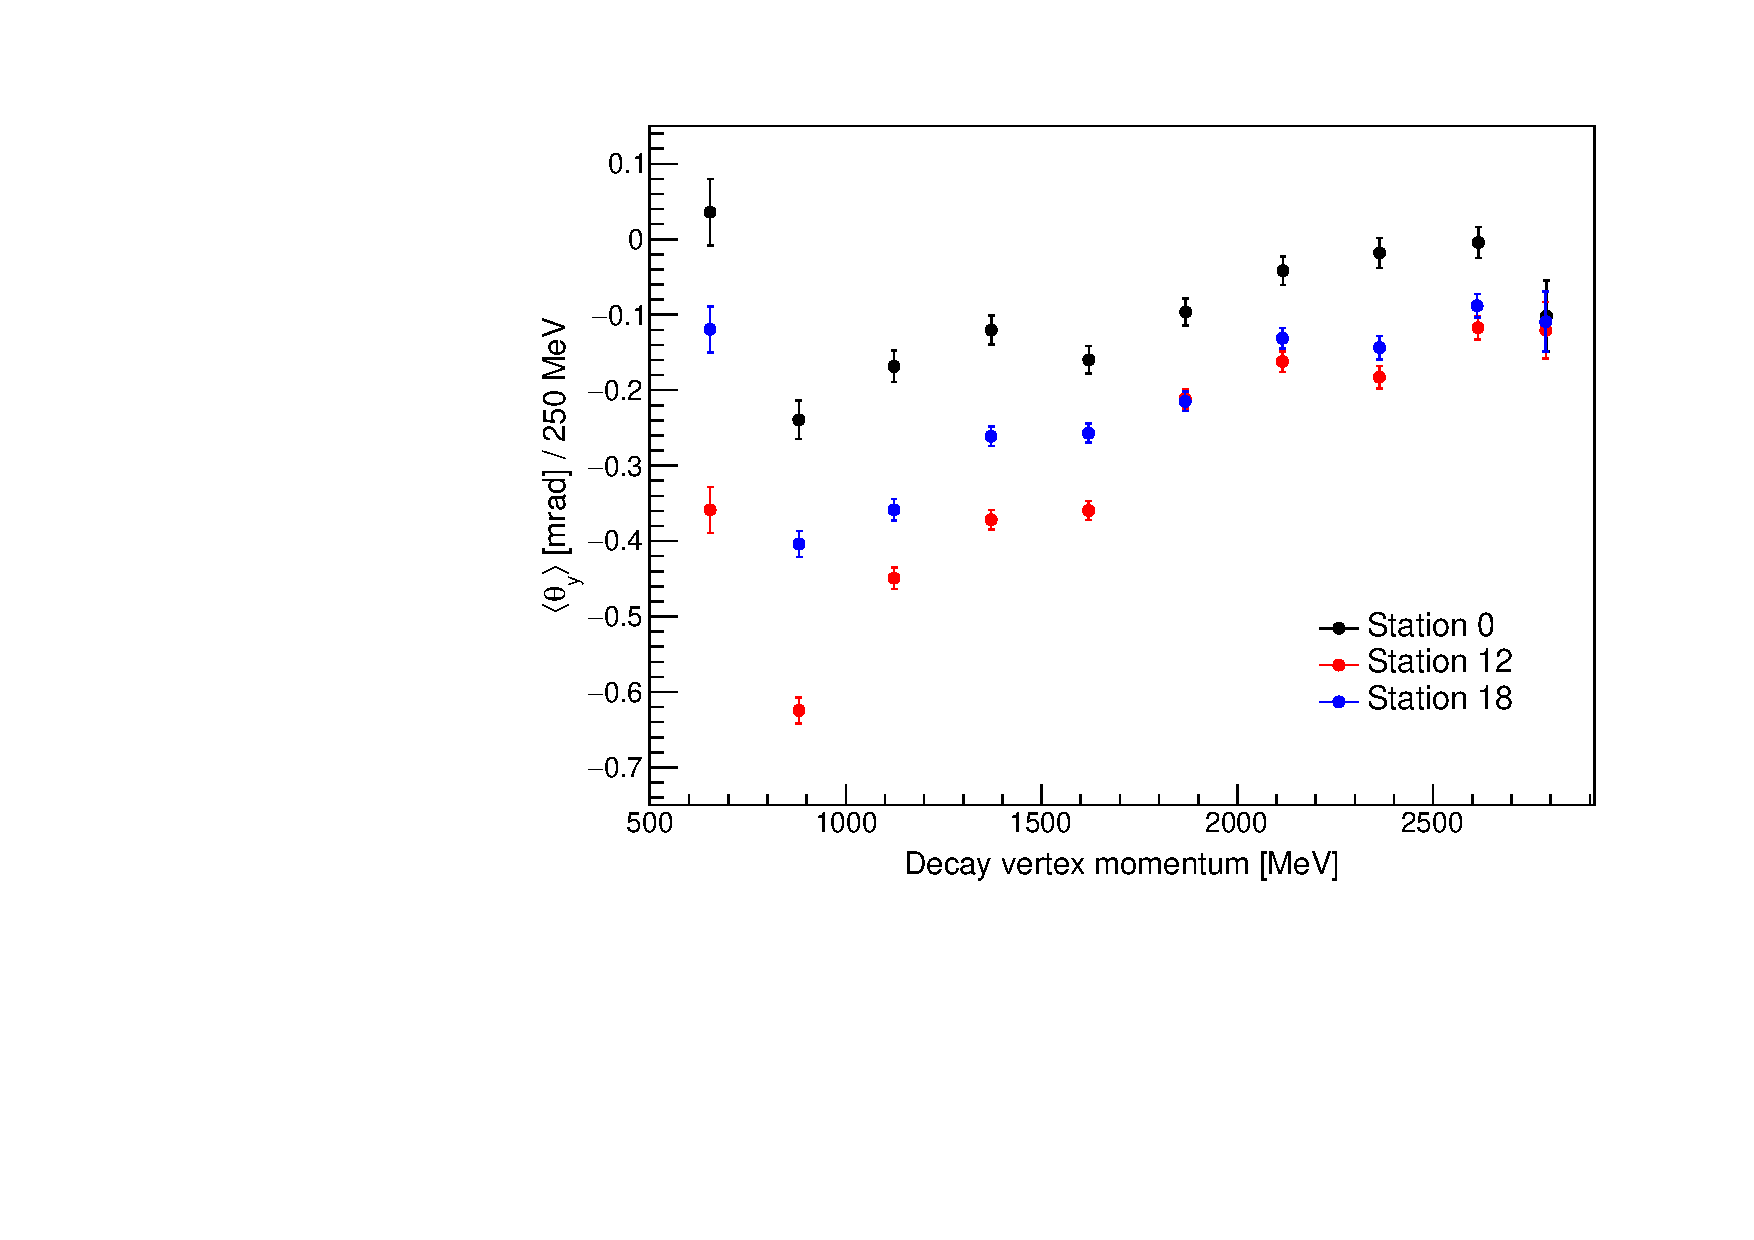
\includegraphics[trim={0 0 0 0},clip,width=.49\textwidth]{Images/Chapter5/VerticalOffsetSimStationOverlay.pdf}\label{subfig:VerticalOffsetSimStationOverlay}}
\caption{The average vertical angle in momentum intervals of 250 MeV, for (a) \textit{all decays} and \textit{reco vertices} (station 12 and station 18 combined), and (b) individual stations including station 0 (for \textit{reco vertices}). Above 500 MeV, this momentum dependence is not present in \textit{all decays}, and is therefore a detector effect. This is partly acceptance related, since it is less pronounced in station 0, which has perfect global alignment in simulation.} 
\label{fig:VerticalOffsetSim}
\end{figure} 

The dependence of $\langle \theta_{y} \rangle$ on momentum is one factor motivating the aforementioned momentum-binned approach to fitting the vertical angle oscillation. In this context, dividing the oscillation into momentum intervals has the effect of reducing the variation in $\langle \theta_{y} \rangle$ with momentum in each fit.  

\subsection{Momentum-binned fits}\label{subsec:MomentumBinnedAnaSim}

\begin{figure}[b!]
\centering{}
\subfloat[]{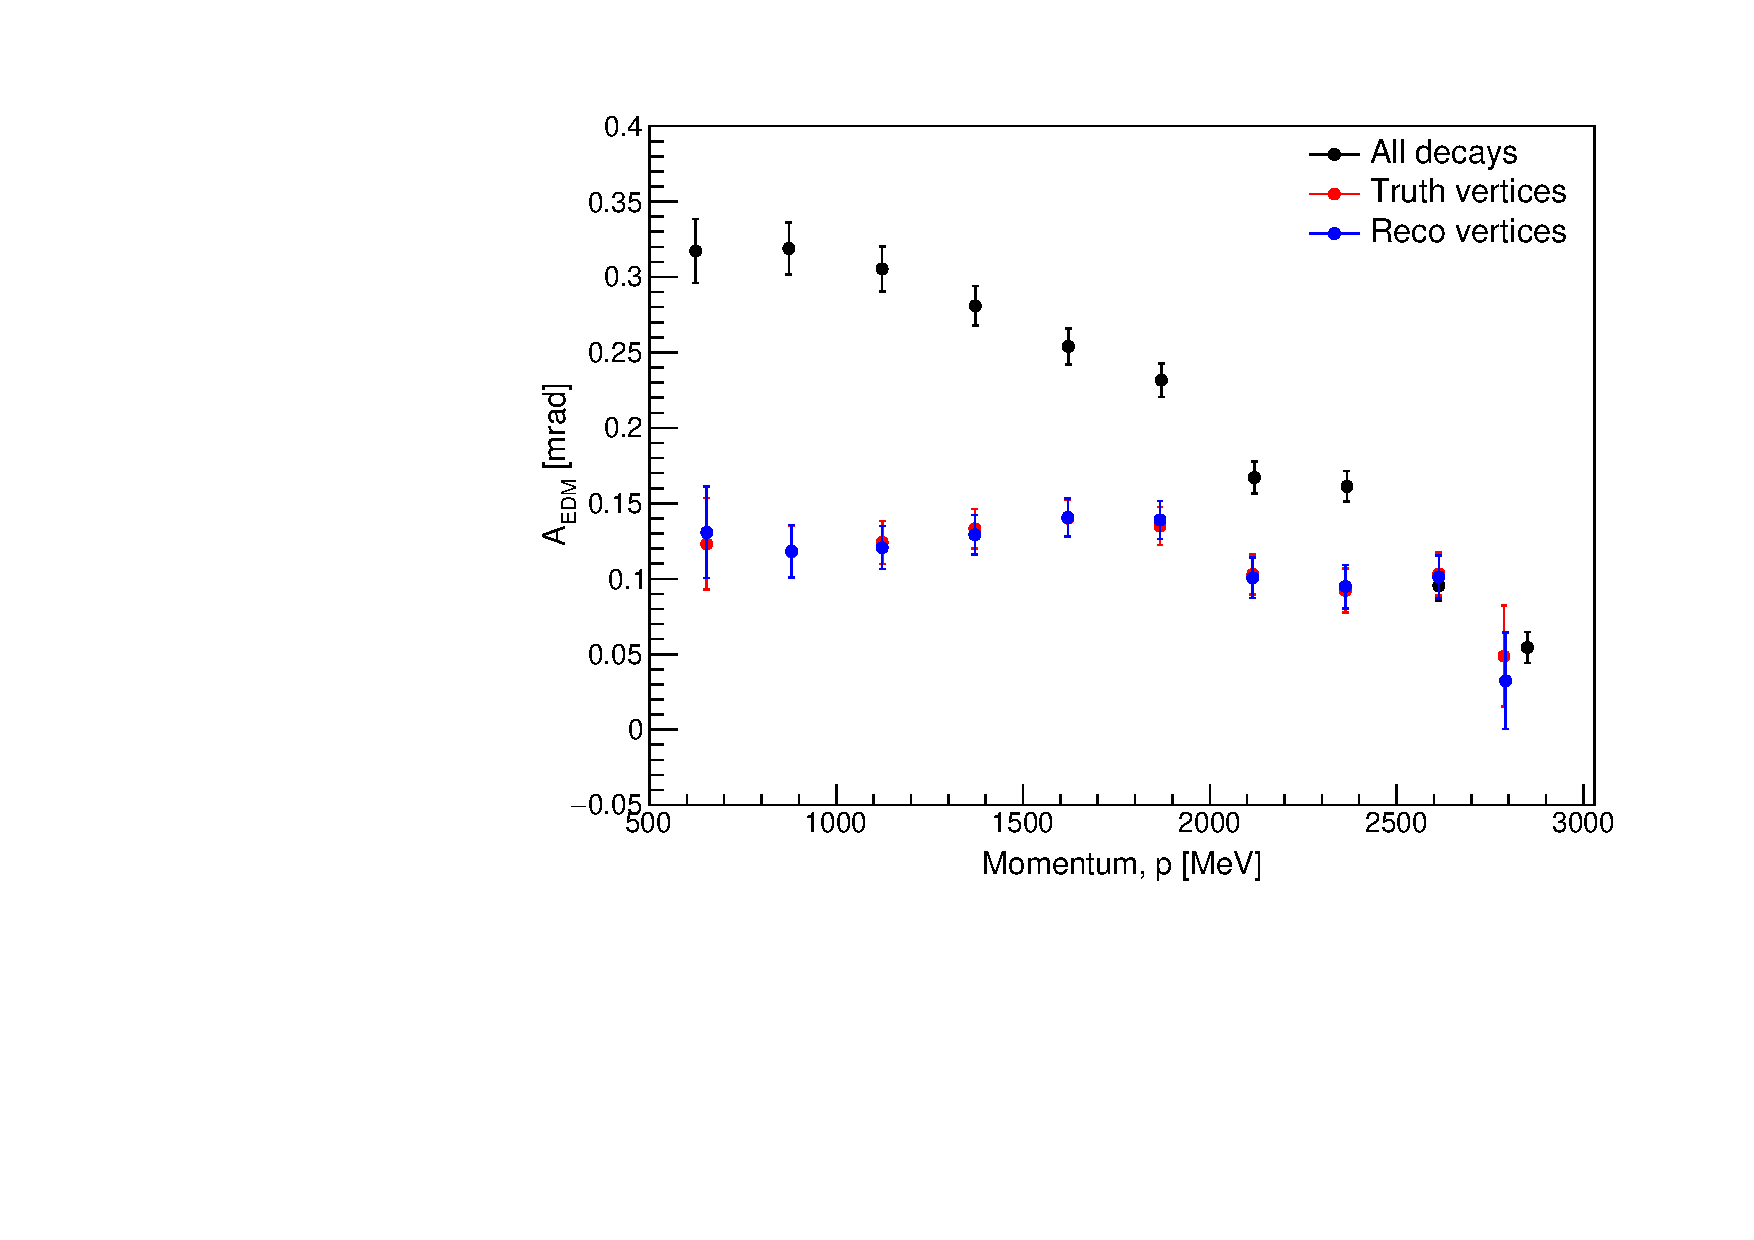
\includegraphics[trim={0 0 0 0},clip,width=.49\textwidth]{Images/Chapter5/S12S18_AEDM_overlay.pdf}\label{subfig:AEDM_overlay_sim}}
\subfloat[]{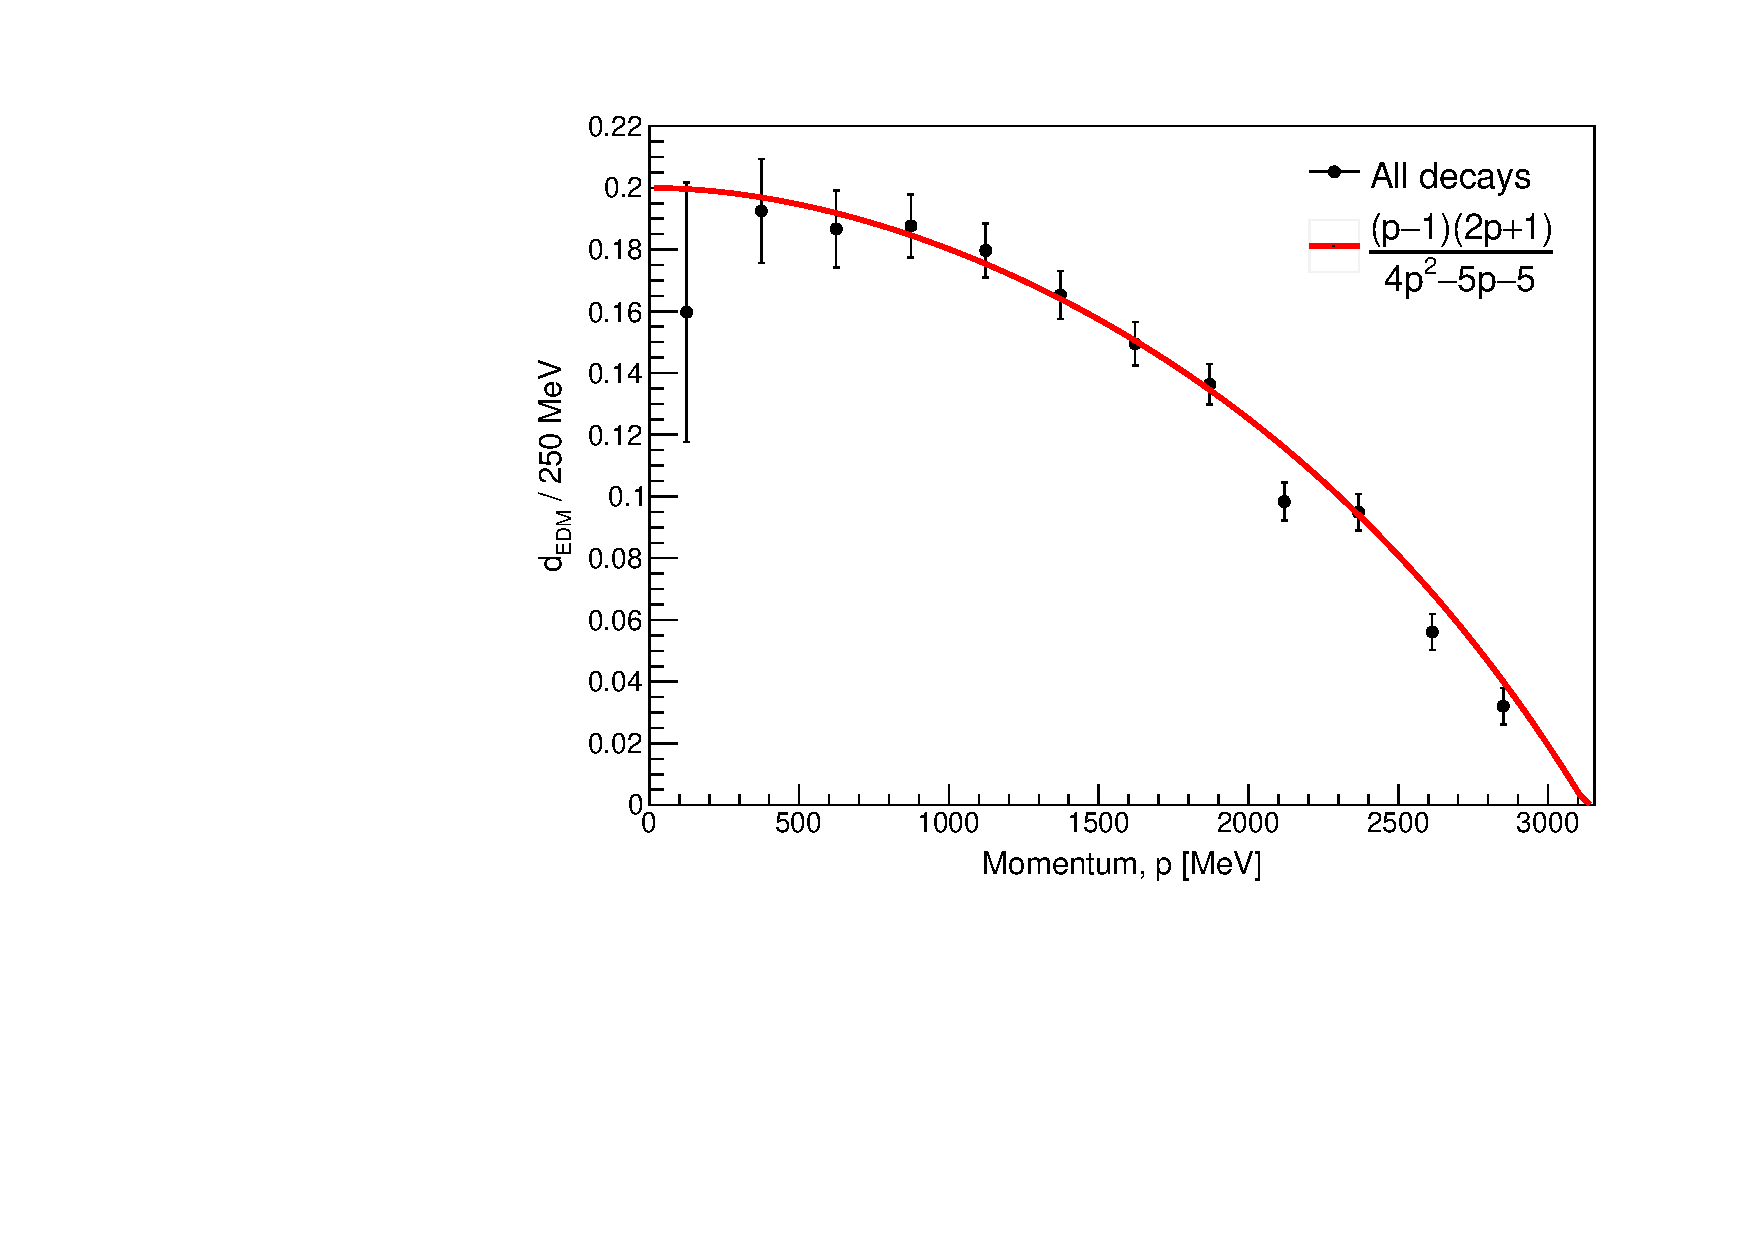
\includegraphics[trim={0 0 0 0},clip,width=.49\textwidth]{Images/Chapter5/AllDecaysFitTest.pdf}\label{subfig:AllDecaysFit}}
\caption{Fit results from the momentum-binned analysis, showing: (a) $A_{\text{EDM}}$ distributed against the mean momentum in each 250 MeV bin; (b) the dilution function, with a normalisation factor of one, overlaid on the tilt angle dilution factor, $d_{\text{EDM}}$, as measured using truth information and 100\% detector acceptance (\textit{all decays}).}
\label{fig:MomentumBinnedSim}
\end{figure} 

\begin{figure}[]
\centering{}
\subfloat[1000-1250 MeV.]{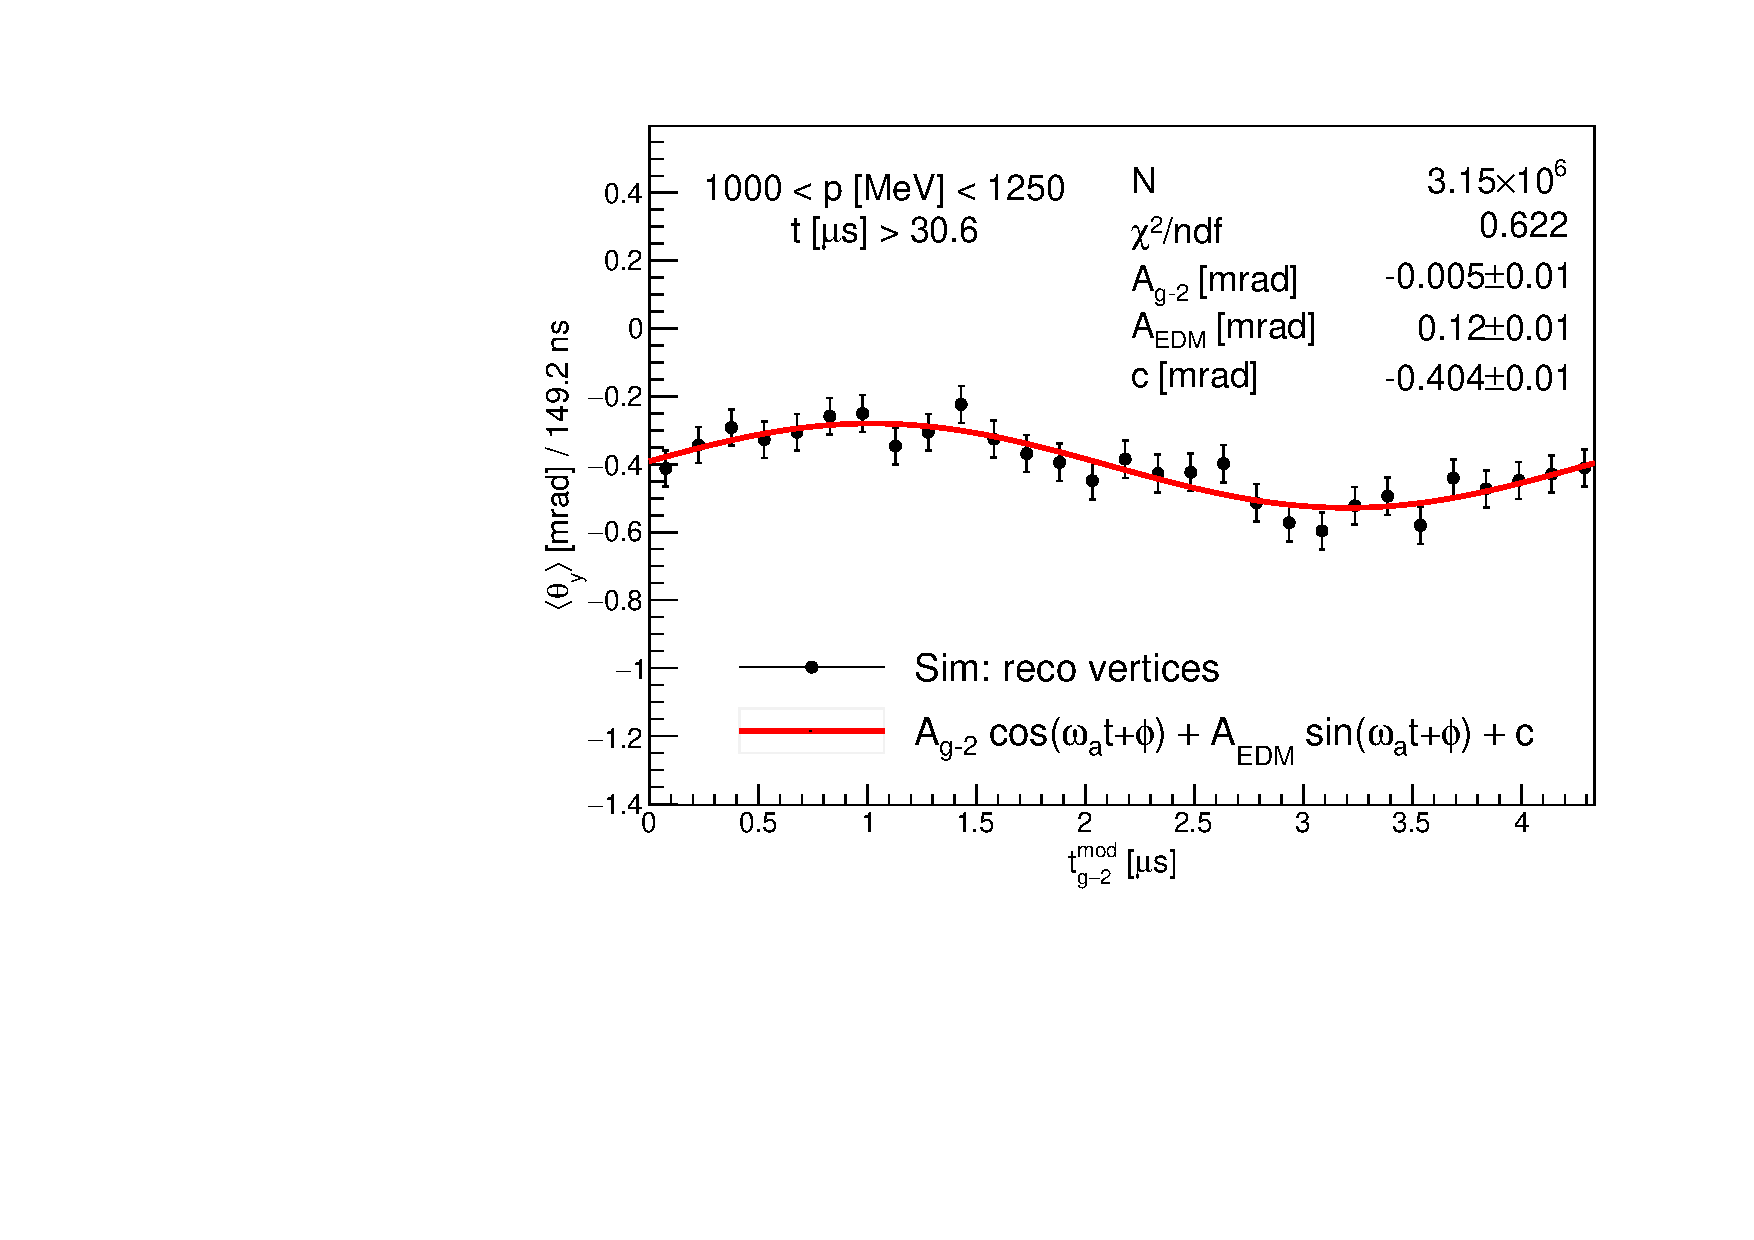
\includegraphics[trim={0 0 0 0},clip,width=.49\textwidth]{Images/Chapter5/S12S18_edmFit_thetaY_1000_1250_trackReco_WORLD_250MeV_BQ_noVertCorr_1.pdf} } 
\subfloat[1250-1500 MeV.]{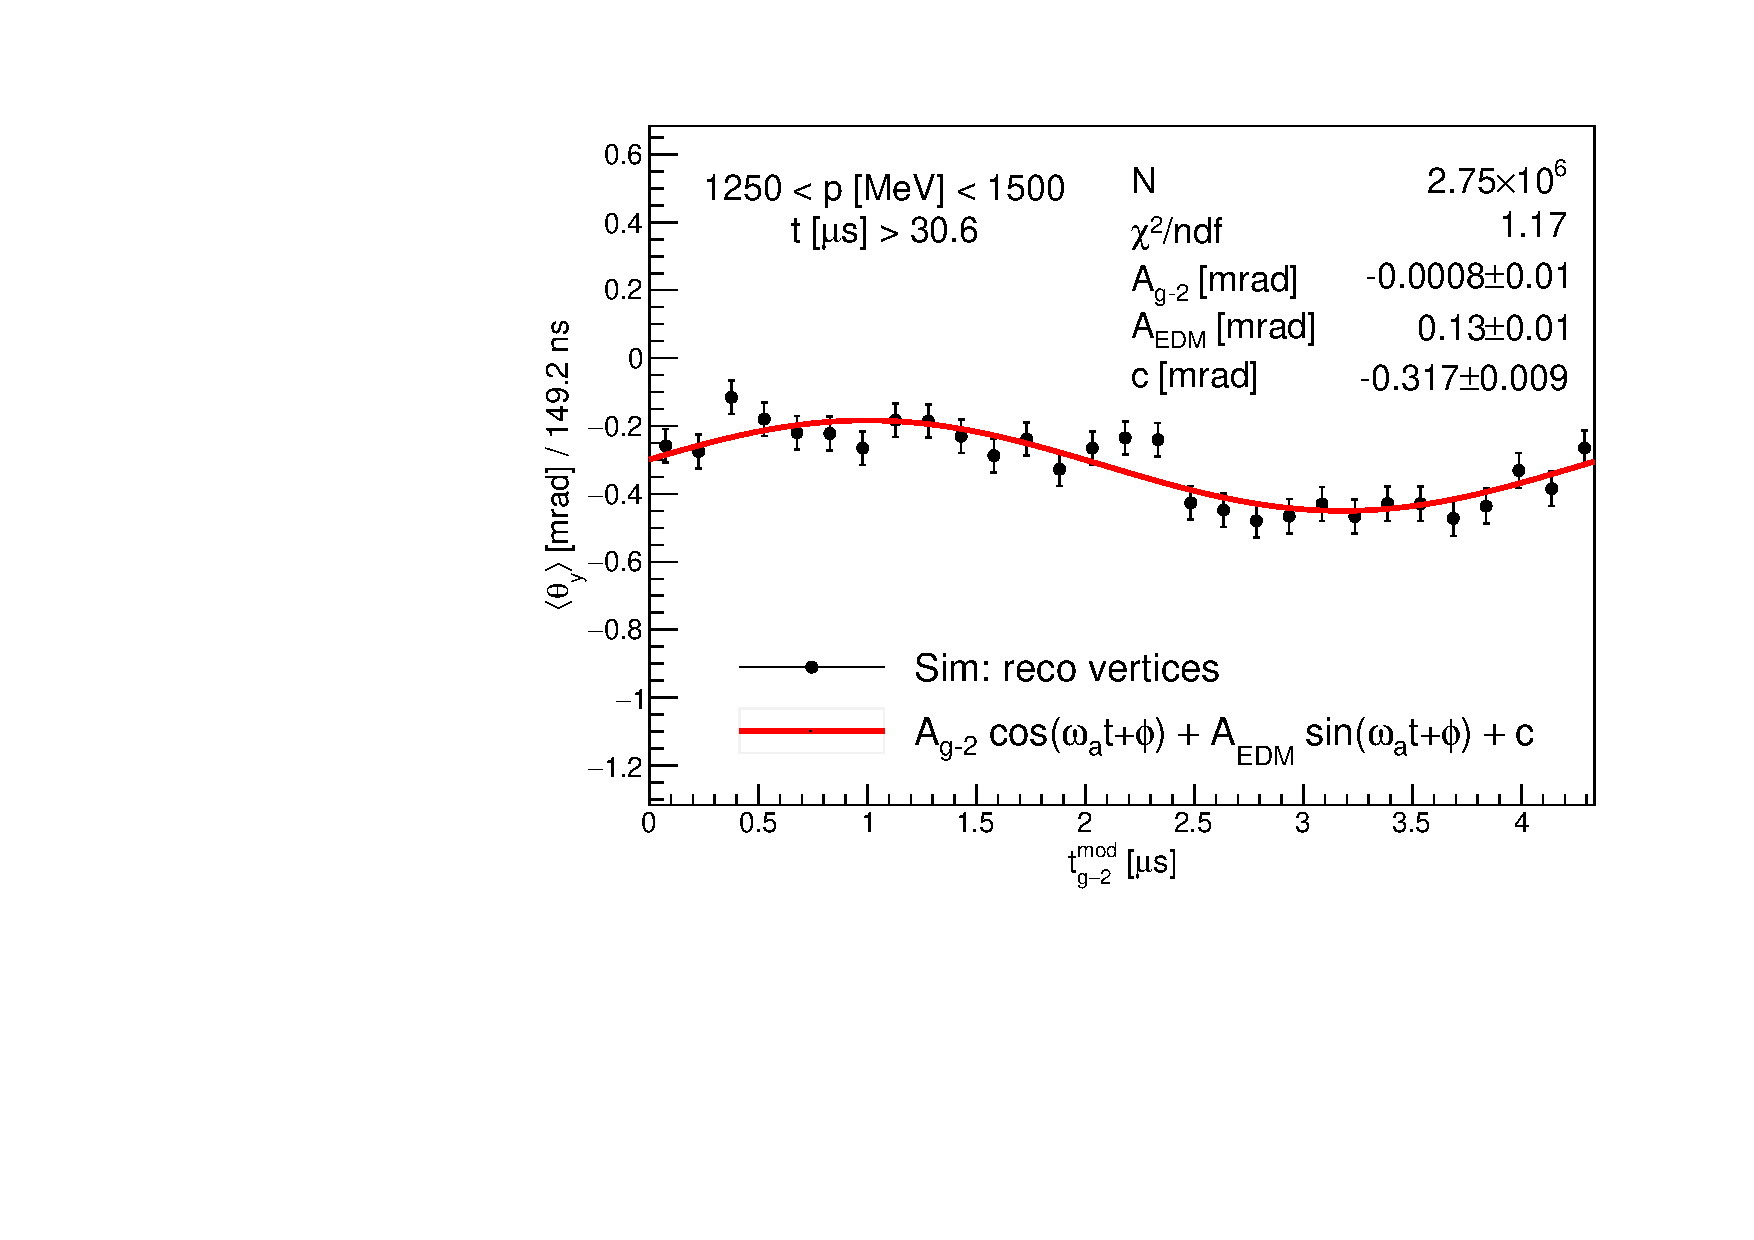
\includegraphics[trim={0 0 0 0},clip,width=.49\textwidth]{Images/Chapter5/S12S18_edmFit_thetaY_1250_1500_trackReco_WORLD_250MeV_BQ_noVertCorr_1.pdf} }
\hfill
\subfloat[1500-1750 MeV.]{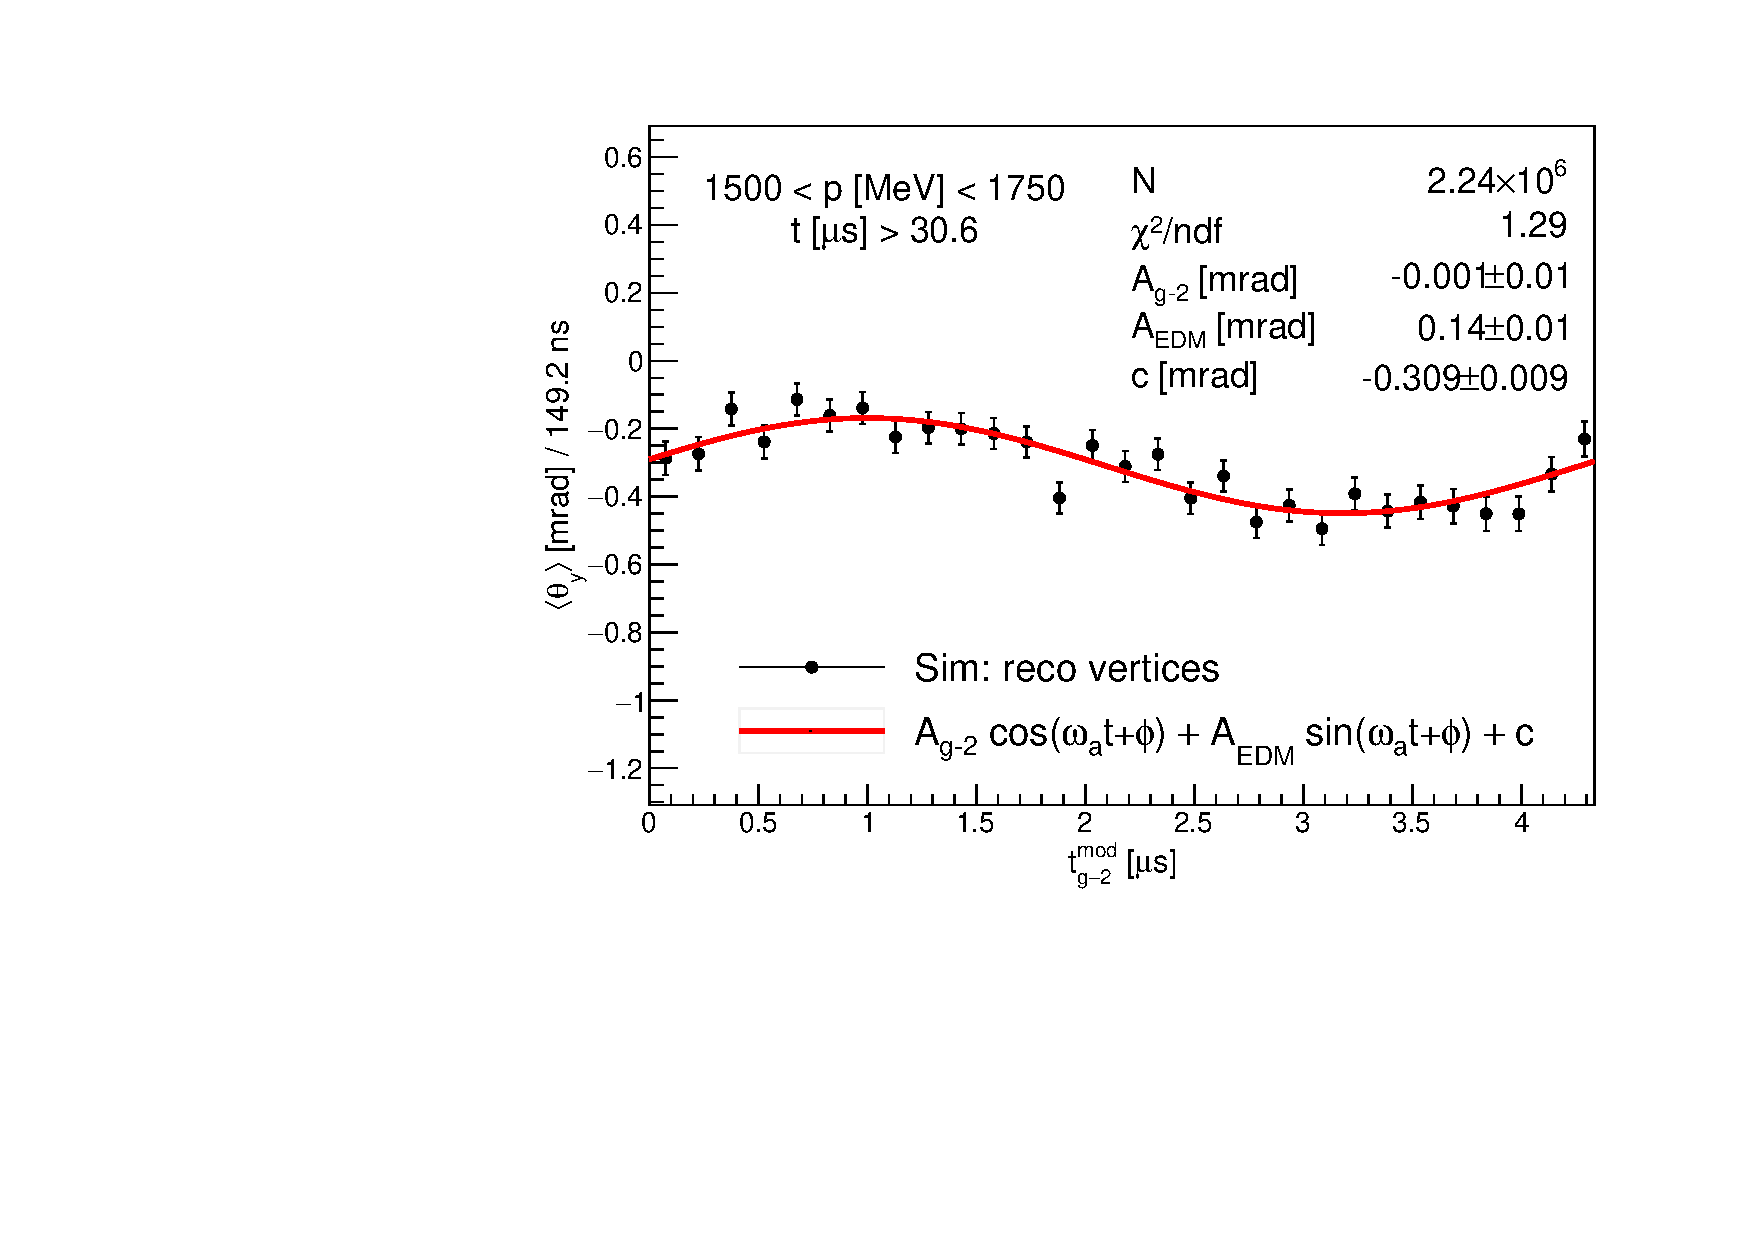
\includegraphics[trim={0 0 0 0},clip,width=.49\textwidth]{Images/Chapter5/S12S18_edmFit_thetaY_1500_1750_trackReco_WORLD_250MeV_BQ_noVertCorr_1.pdf} }
\subfloat[1750-2000 MeV.]{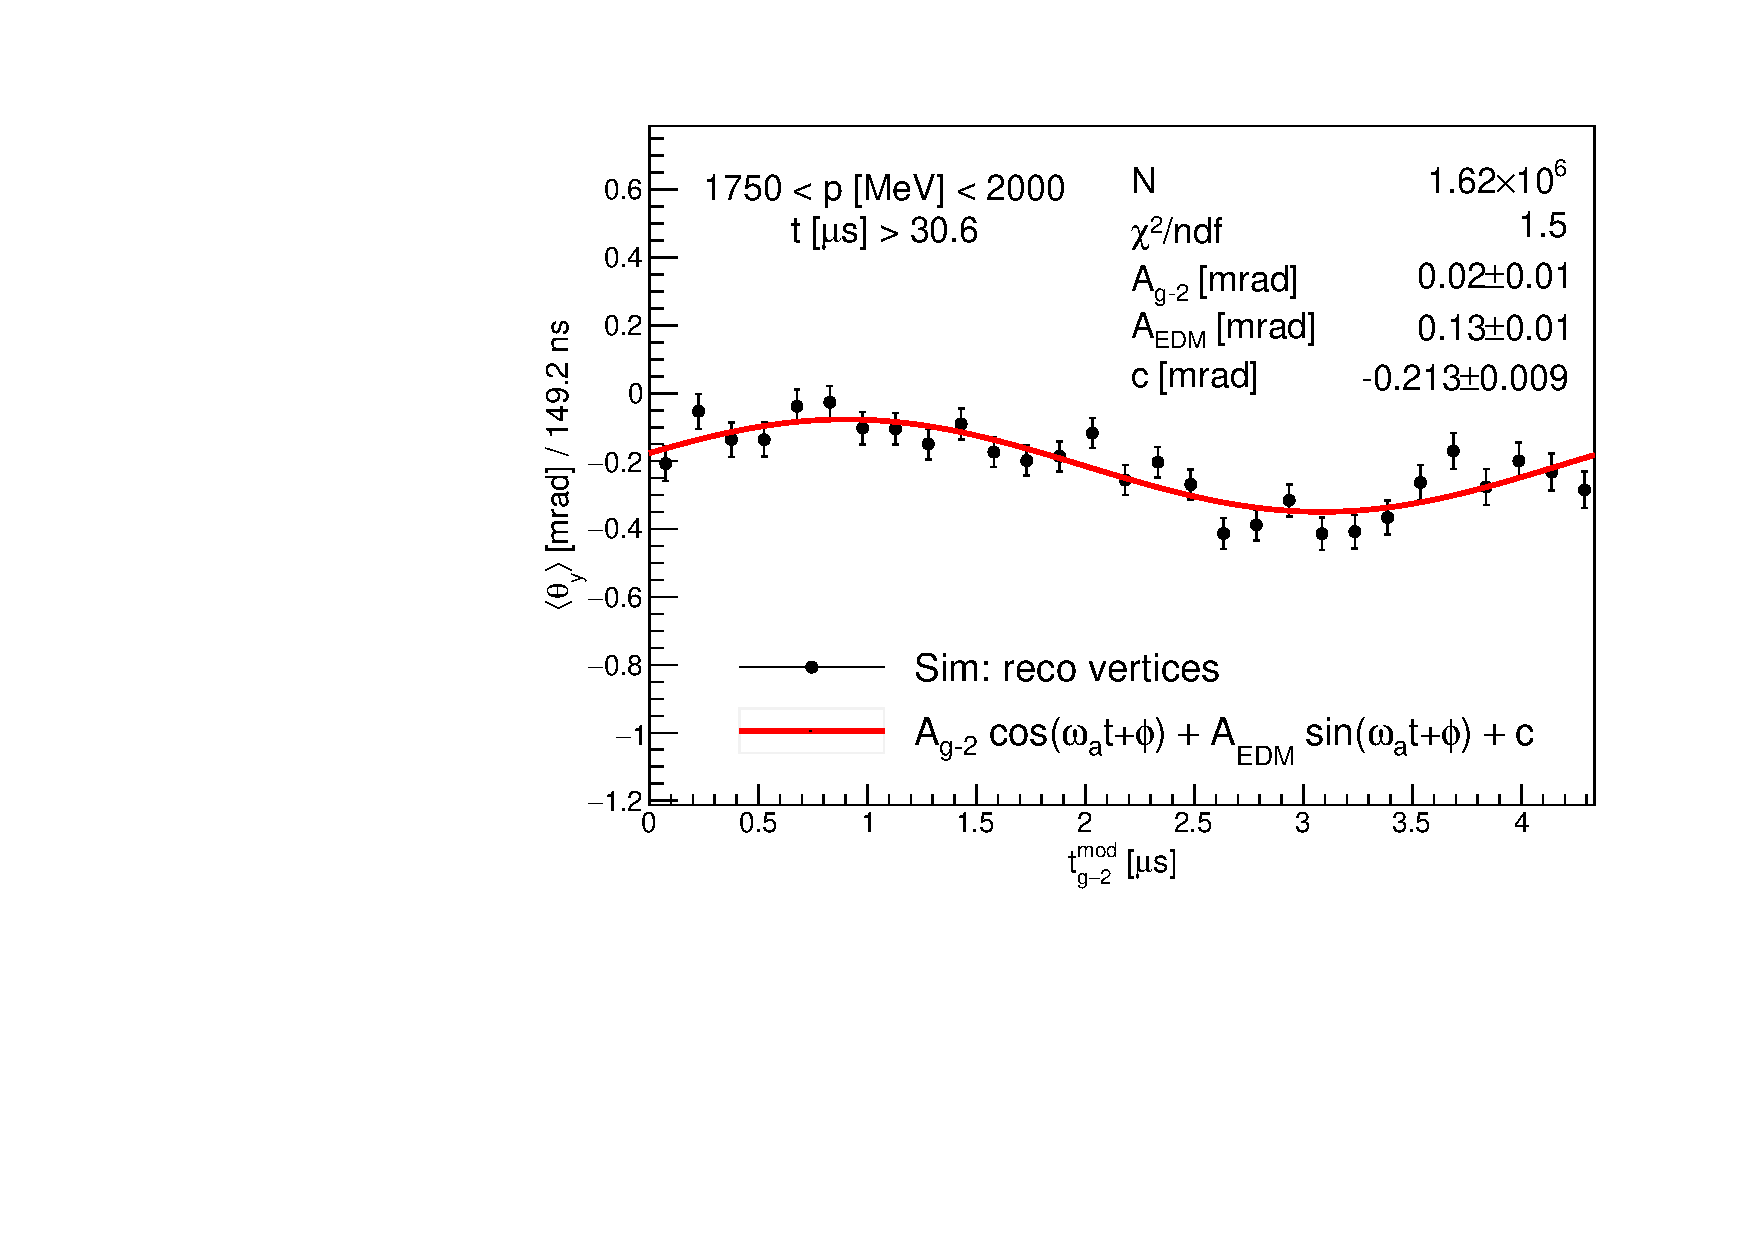
\includegraphics[trim={0 0 0 0},clip,width=.49\textwidth]{Images/Chapter5/S12S18_edmFit_thetaY_1750_2000_trackReco_WORLD_250MeV_BQ_noVertCorr_1.pdf} }
\hfill
\subfloat[2000-2250 MeV.]{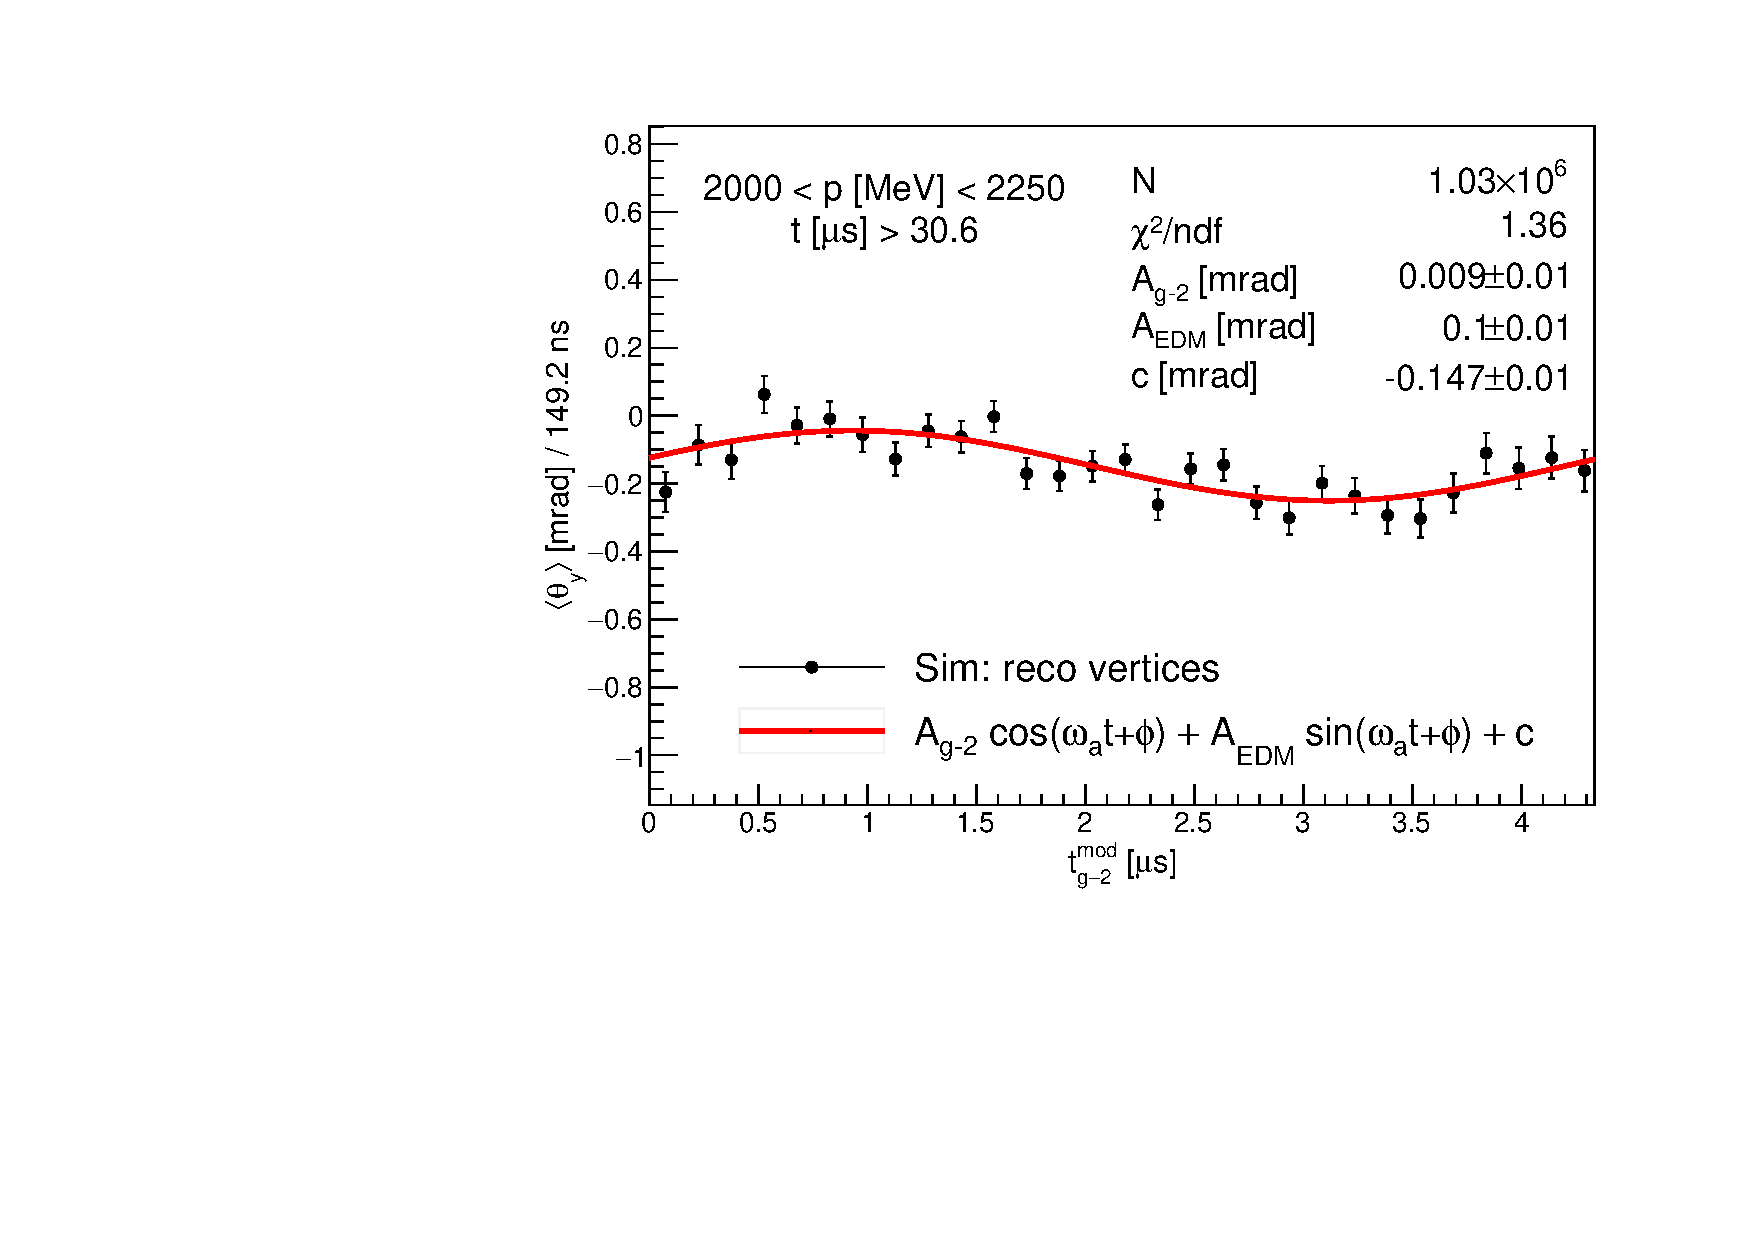
\includegraphics[trim={0 0 0 0},clip,width=.49\textwidth]{Images/Chapter5/S12S18_edmFit_thetaY_2000_2250_trackReco_WORLD_250MeV_BQ_noVertCorr_1.pdf} }
\subfloat[2250-2500 MeV.]{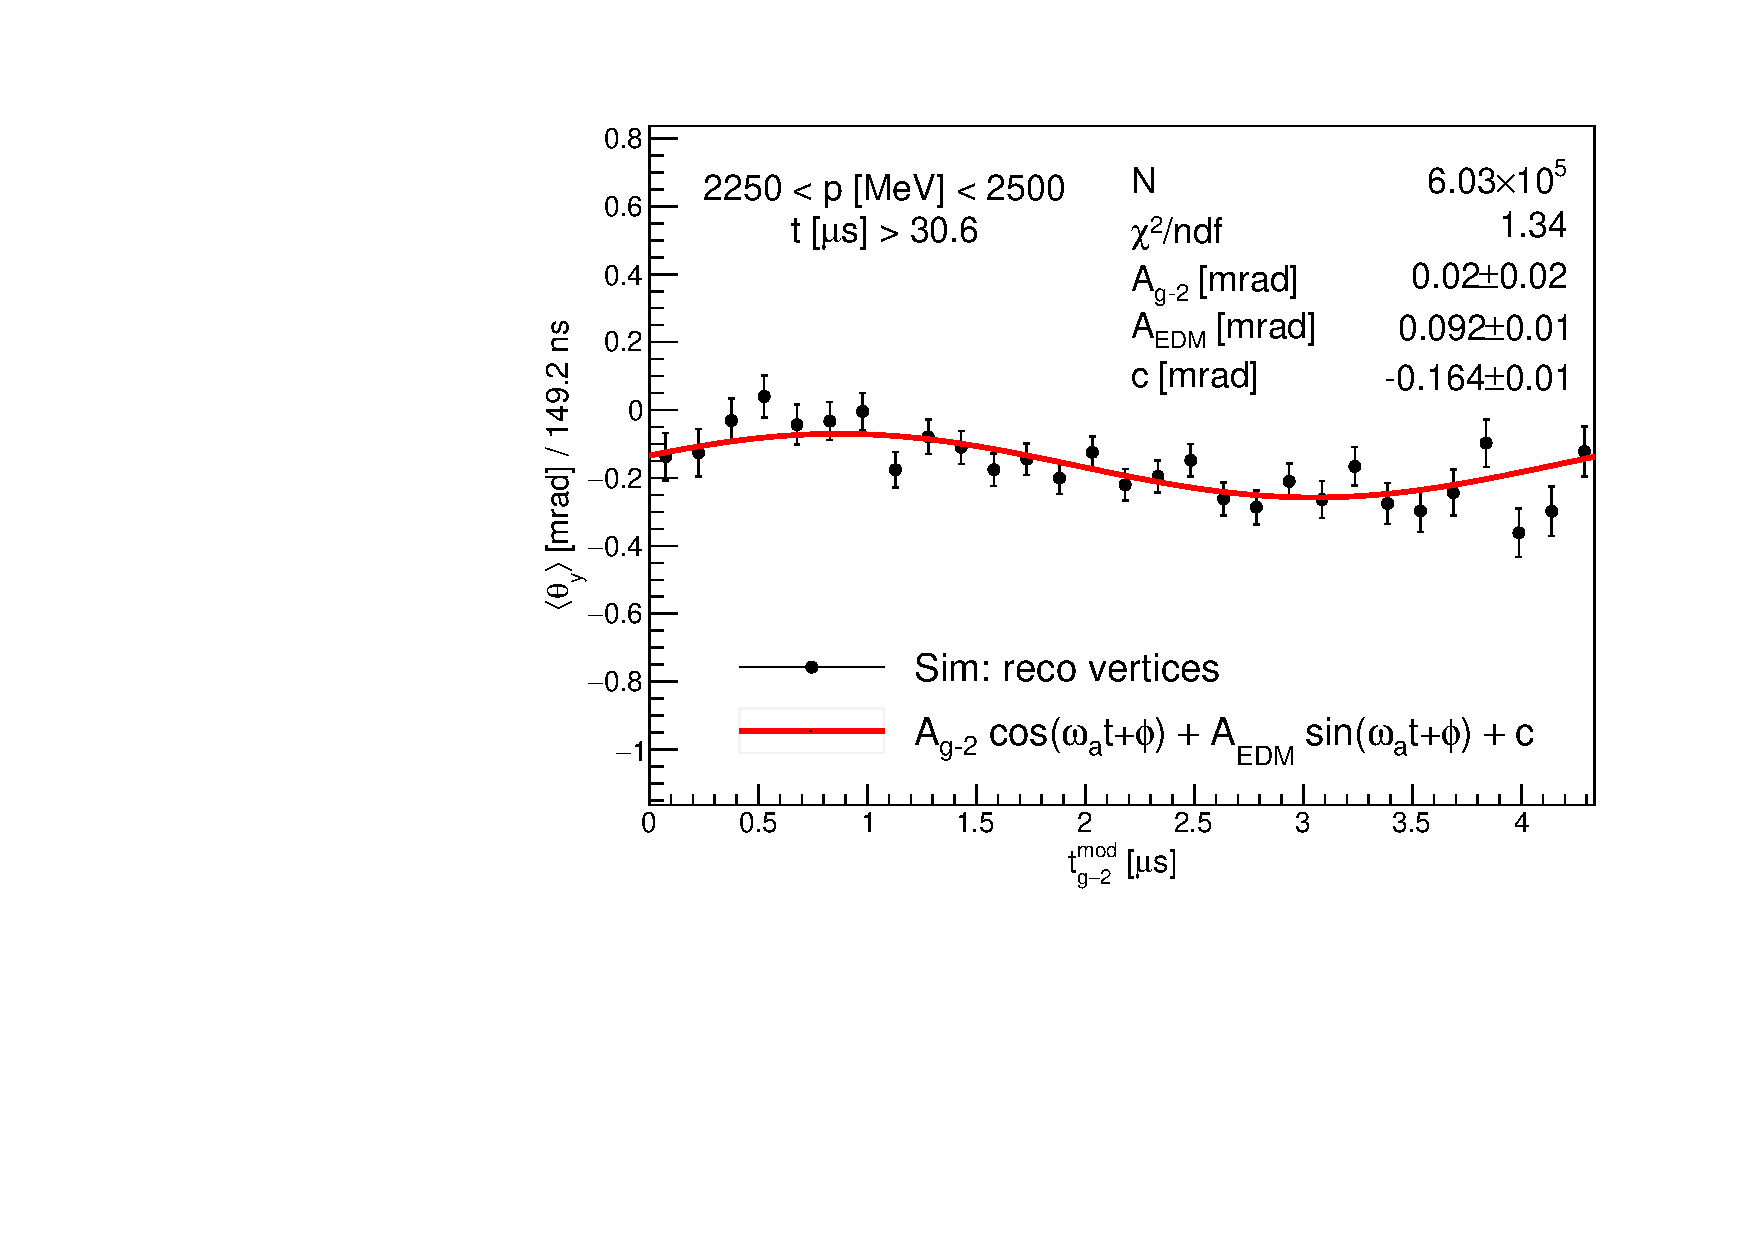
\includegraphics[trim={0 0 0 0},clip,width=.49\textwidth]{Images/Chapter5/S12S18_edmFit_thetaY_2250_2500_trackReco_WORLD_250MeV_BQ_noVertCorr_1.pdf} }
\caption{Momentum-binned vertical angle oscillation fits for the \textit{reco vertices} reconstruction. Tracker stations 12 and 18 are combined.}
\label{fig:TrackRecoMomBinnedFits}
\end{figure}

Fits to the average vertical angle oscillation in momentum intervals of 250 MeV, using the \textit{reco vertices} reconstruction of the 30$\times$ BNL sample, are presented in Figure \ref{fig:TrackRecoMomBinnedFits}. Besides the momentum binning, the fitting procedure is identical to that described in Section \ref{subsec:BasicVertAngFitsSim}, and the same values of $\phi$ are used as are reported in Table \ref{tbl:BasicSimFits}.

The measured values of $A_{\text{EDM}}$ for each of the three reconstructions are distributed over the range of 500-3000 MeV in Figure \ref{subfig:AEDM_overlay_sim}. An overall reduction in $A_{\text{EDM}}$ with increasing momentum is present in all samples, as expected from the momentum dependent dilution function given by Equation \ref{eqn:DilutionFunction2}. The impact of tracker acceptance is clear, manifesting as a significant decrease in sensitivity in the tracked samples compared to the \textit{all decays} sample, which is most pronounced at low momentum. 

\subsection{Verifying the dilution function}

The aforementioned dilution function, Equation \ref{eqn:DilutionFunction2}, describes the variation in $A_{\text{EDM}}$ with momentum in the case of 100\% detector acceptance. This expression is vital in the extraction of the tilt angle, $\delta$, from the measured values of $A_{\text{EDM}}$ per momentum bin, and so must be verified. To accomplish this, $A_{\text{EDM}}$ per 250 MeV, measured from the \textit{all decays} reconstruction, was converted to dilution, $d_{\text{EDM}}$, according to the aforementioned inputted $\delta$ of 1.69 mrad. The dilution function was then overlaid on the simulated distribution of $d_{\text{EDM}}$, demonstrating good agreement as shown by Figure \ref{subfig:AllDecaysFit}. 

\section{Tracker acceptance characterisation}\label{sec:AcceptanceSim}

By comparison of fit results from \textit{all decays} to those from track vertices, presented in the previous section, it may be deduced that tracker acceptance plays a critical role in the observed dilution of the tilt angle. In this section, the impact of tracker vertical angle acceptance on the measured $A_{\text{EDM}}$ as a function of momentum will be characterised.


% , in part by use an additional, pre-existing, sample of Monte Carlo with no injected EDM. In this `No EDM' sample, the true extrapolated track vertices are a subset of the truth decay parameters. This is essential when counting the fraction of accepted decays, and is not the case for the simulation datasets detailed in the earlier sections of this chapter.

% by use a separate, pre-existing, sample of Monte Carlo with no injected EDM. In this sample, the true extrapolated track vertices, `truth vertices', are a subset of the truth decay parameters, again labelled `all decays'. This is essential when counting the fraction of accepted decays, and is not the case for the simulation datasets detailed in the earlier sections of this chapter.

\subsection{Vertical angle acceptance}

\begin{figure}[b!]
\centering{}
\subfloat[Radial.]{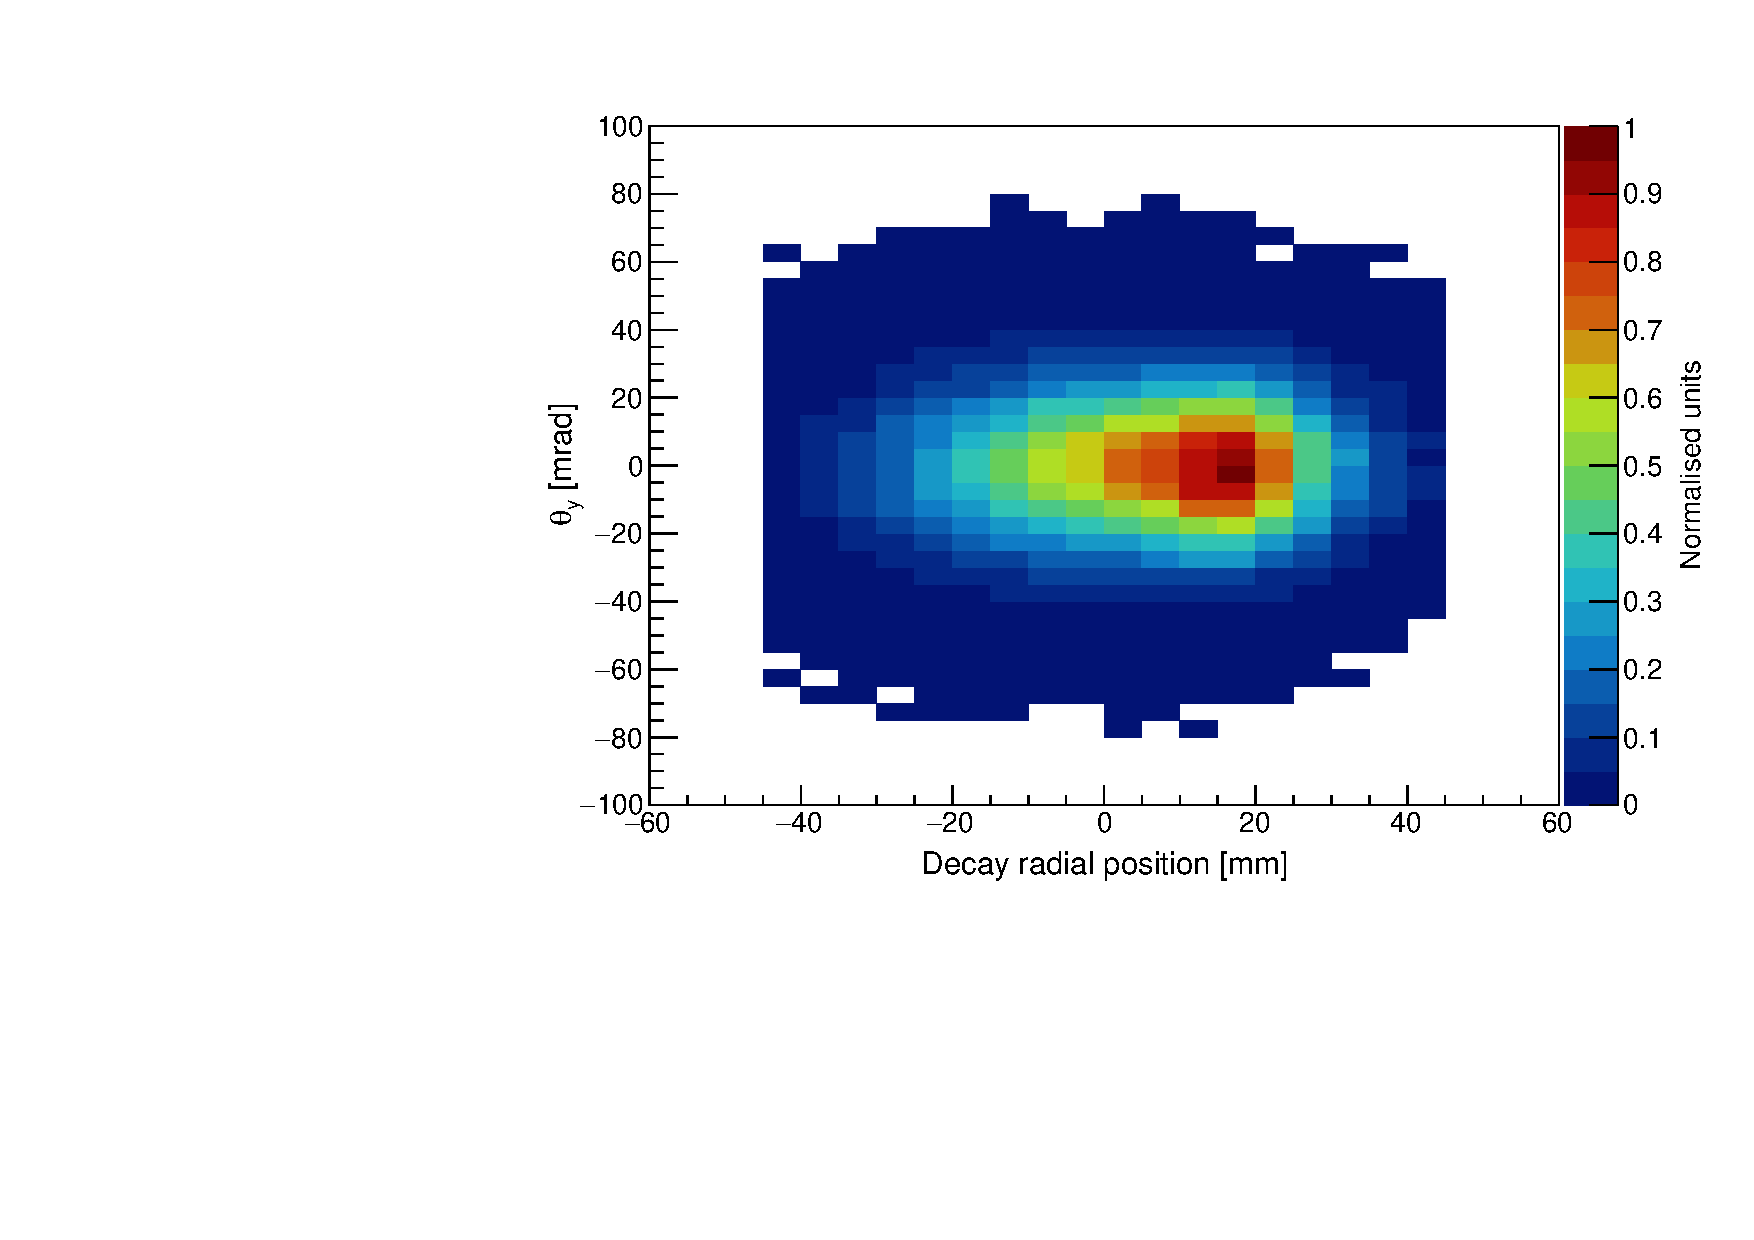
\includegraphics[trim={0 0 0 0},clip,width=.33\textwidth]{Images/Chapter5/S12_thetaY_vs_R_tracks_0_3127_MeV.pdf}}
\subfloat[Azimuthal.]{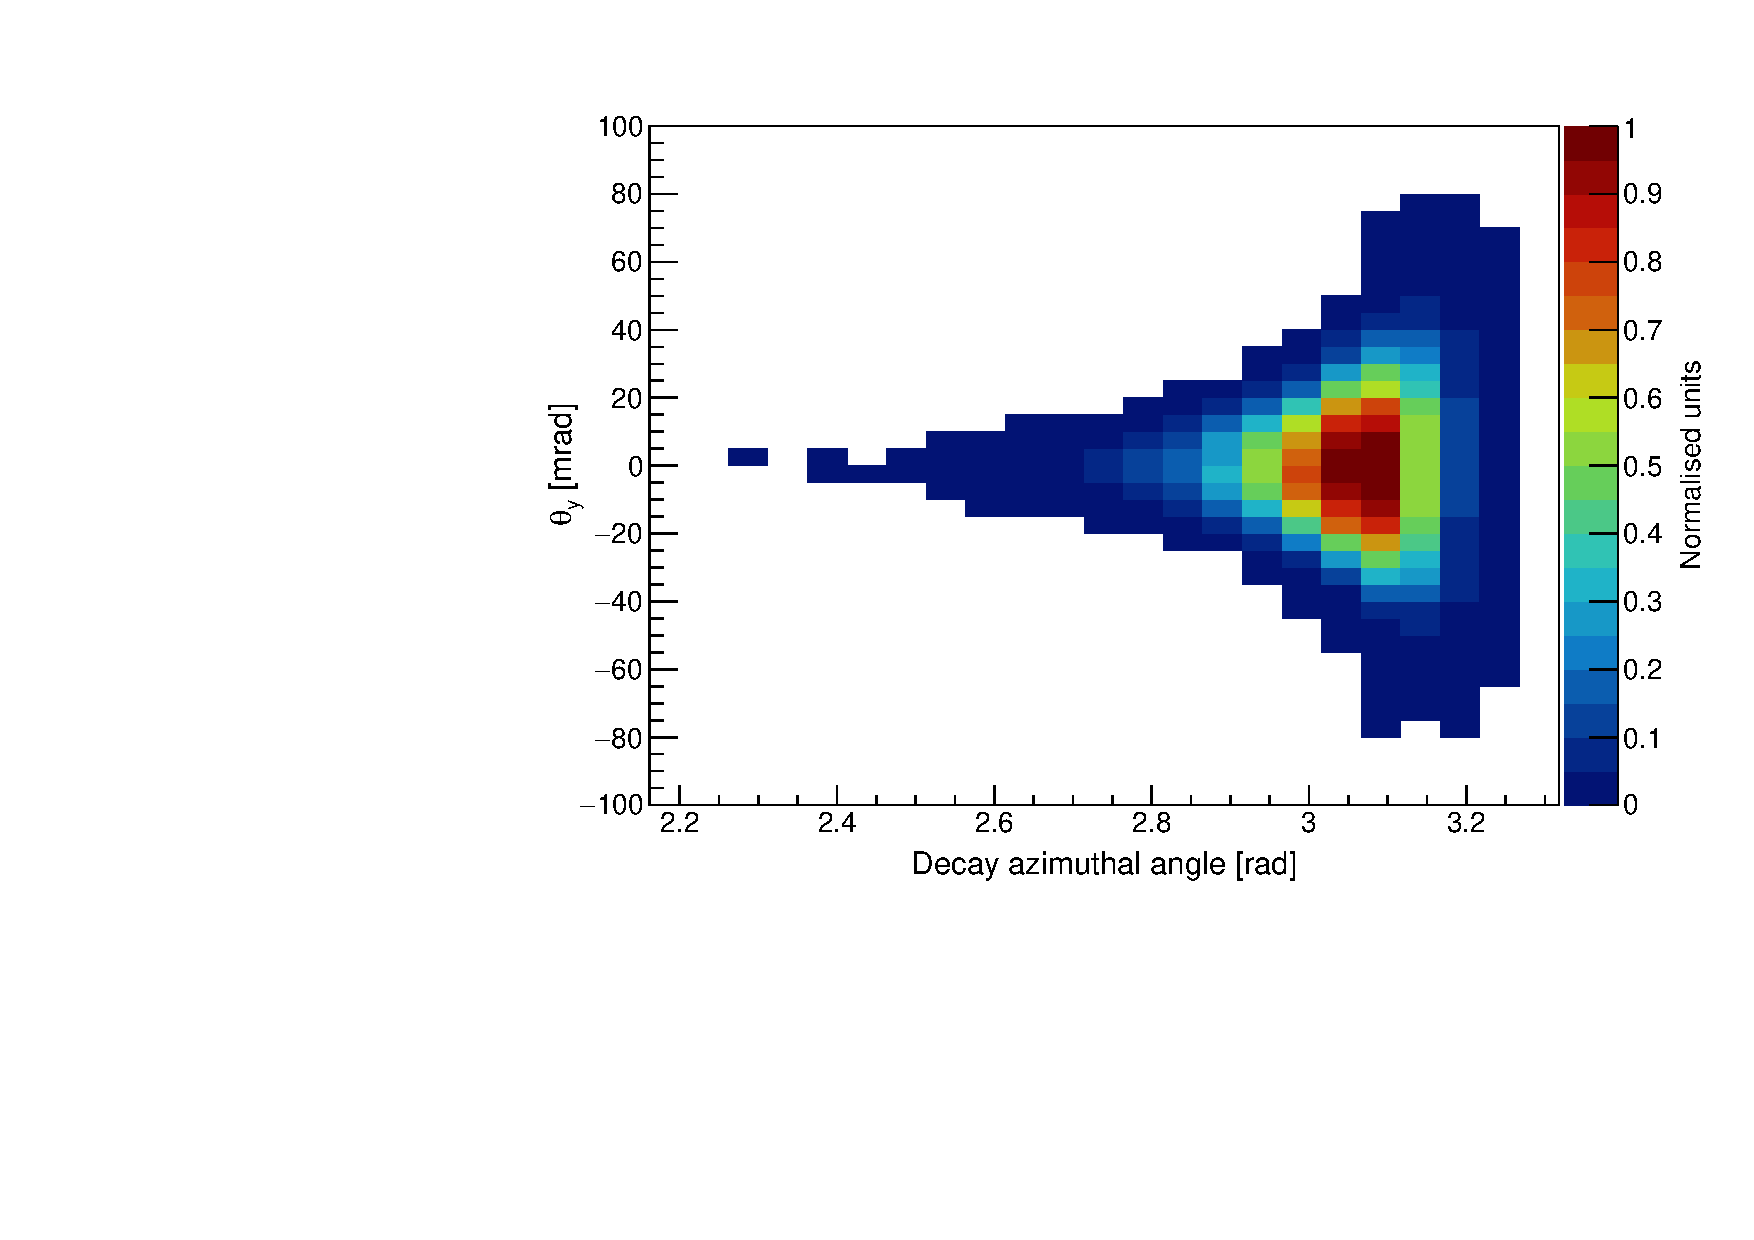
\includegraphics[trim={0 0 0 0},clip,width=.33\textwidth]{Images/Chapter5/S12_thetaY_vs_Phi_tracks_0_3127_MeV.pdf}}
\subfloat[Vertical.]{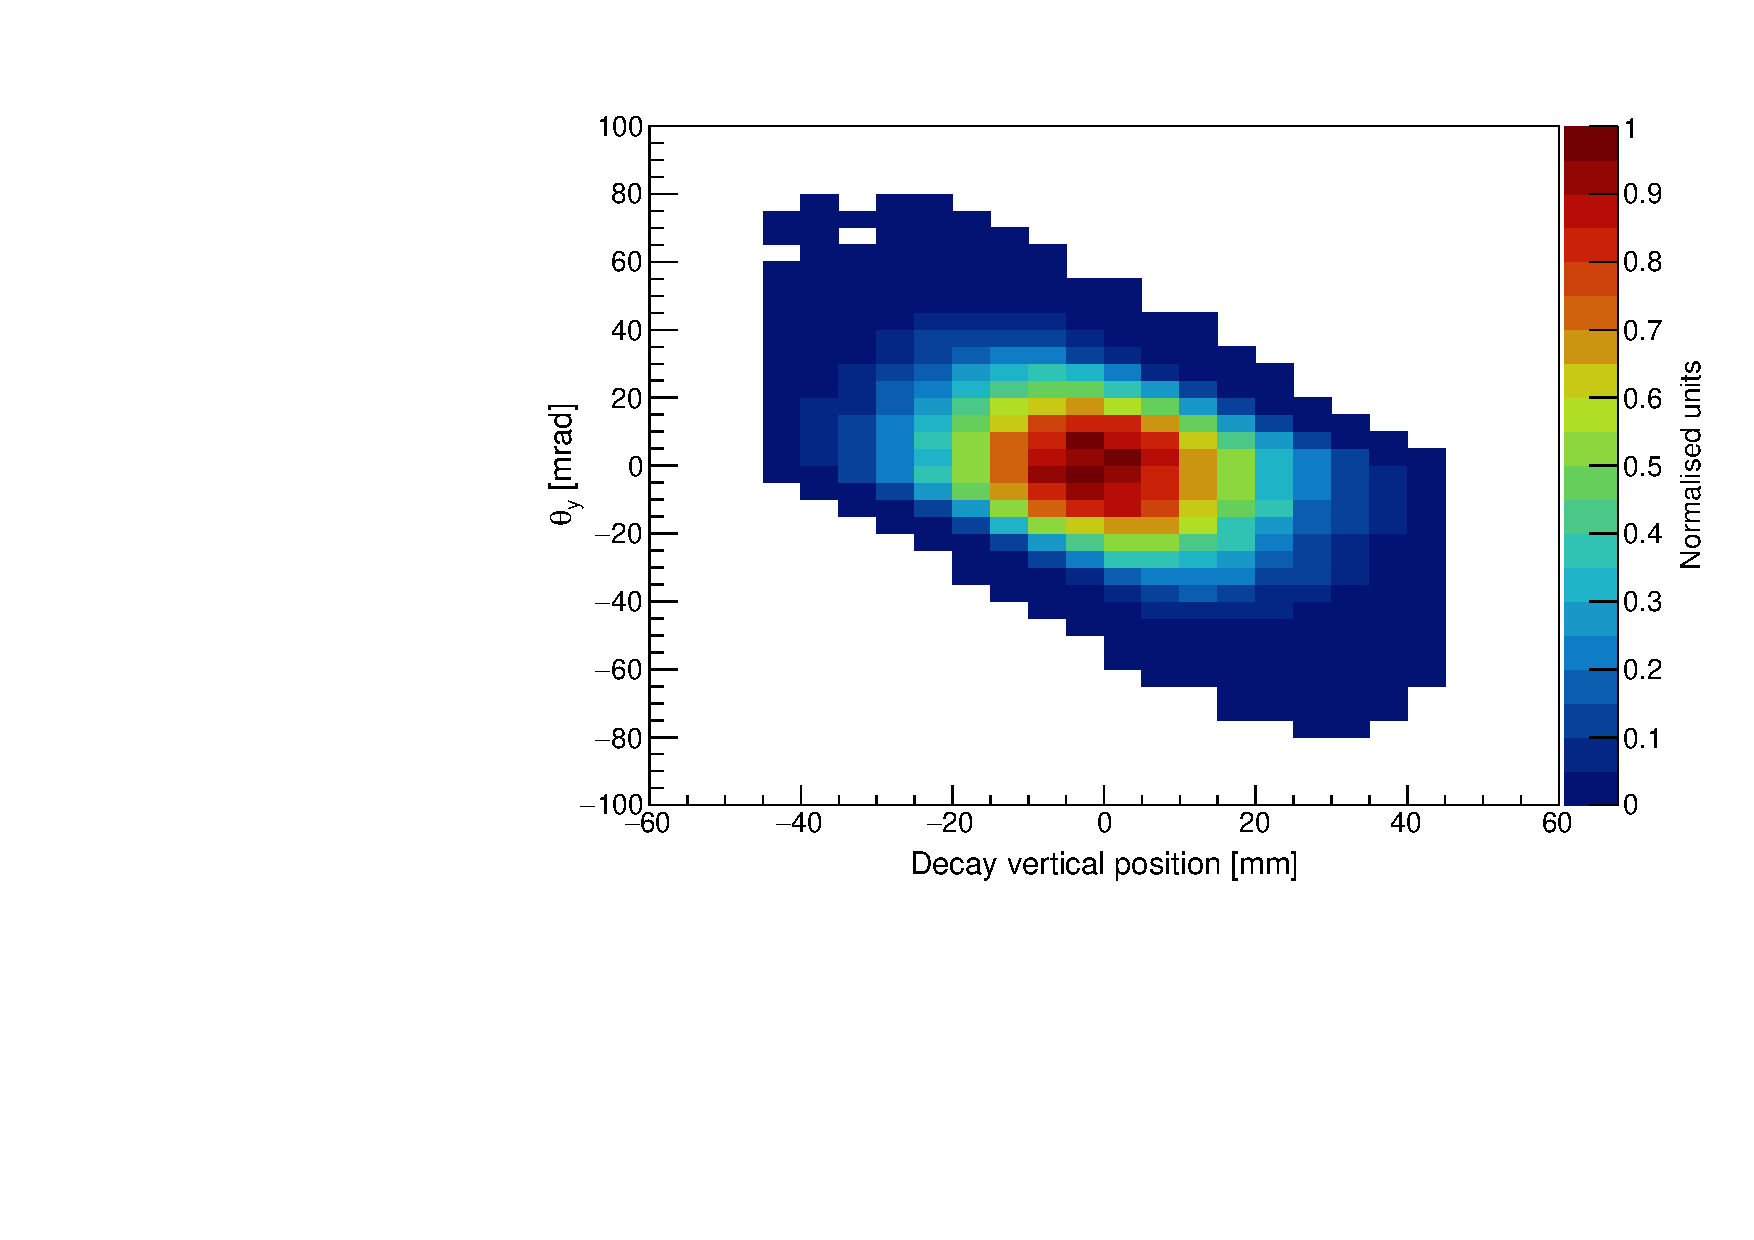
\includegraphics[trim={0 0 0 0},clip,width=.33\textwidth]{Images/Chapter5/S12_thetaY_vs_Y_tracks_0_3127_MeV.pdf}}
\hfill
\subfloat[Radial.]{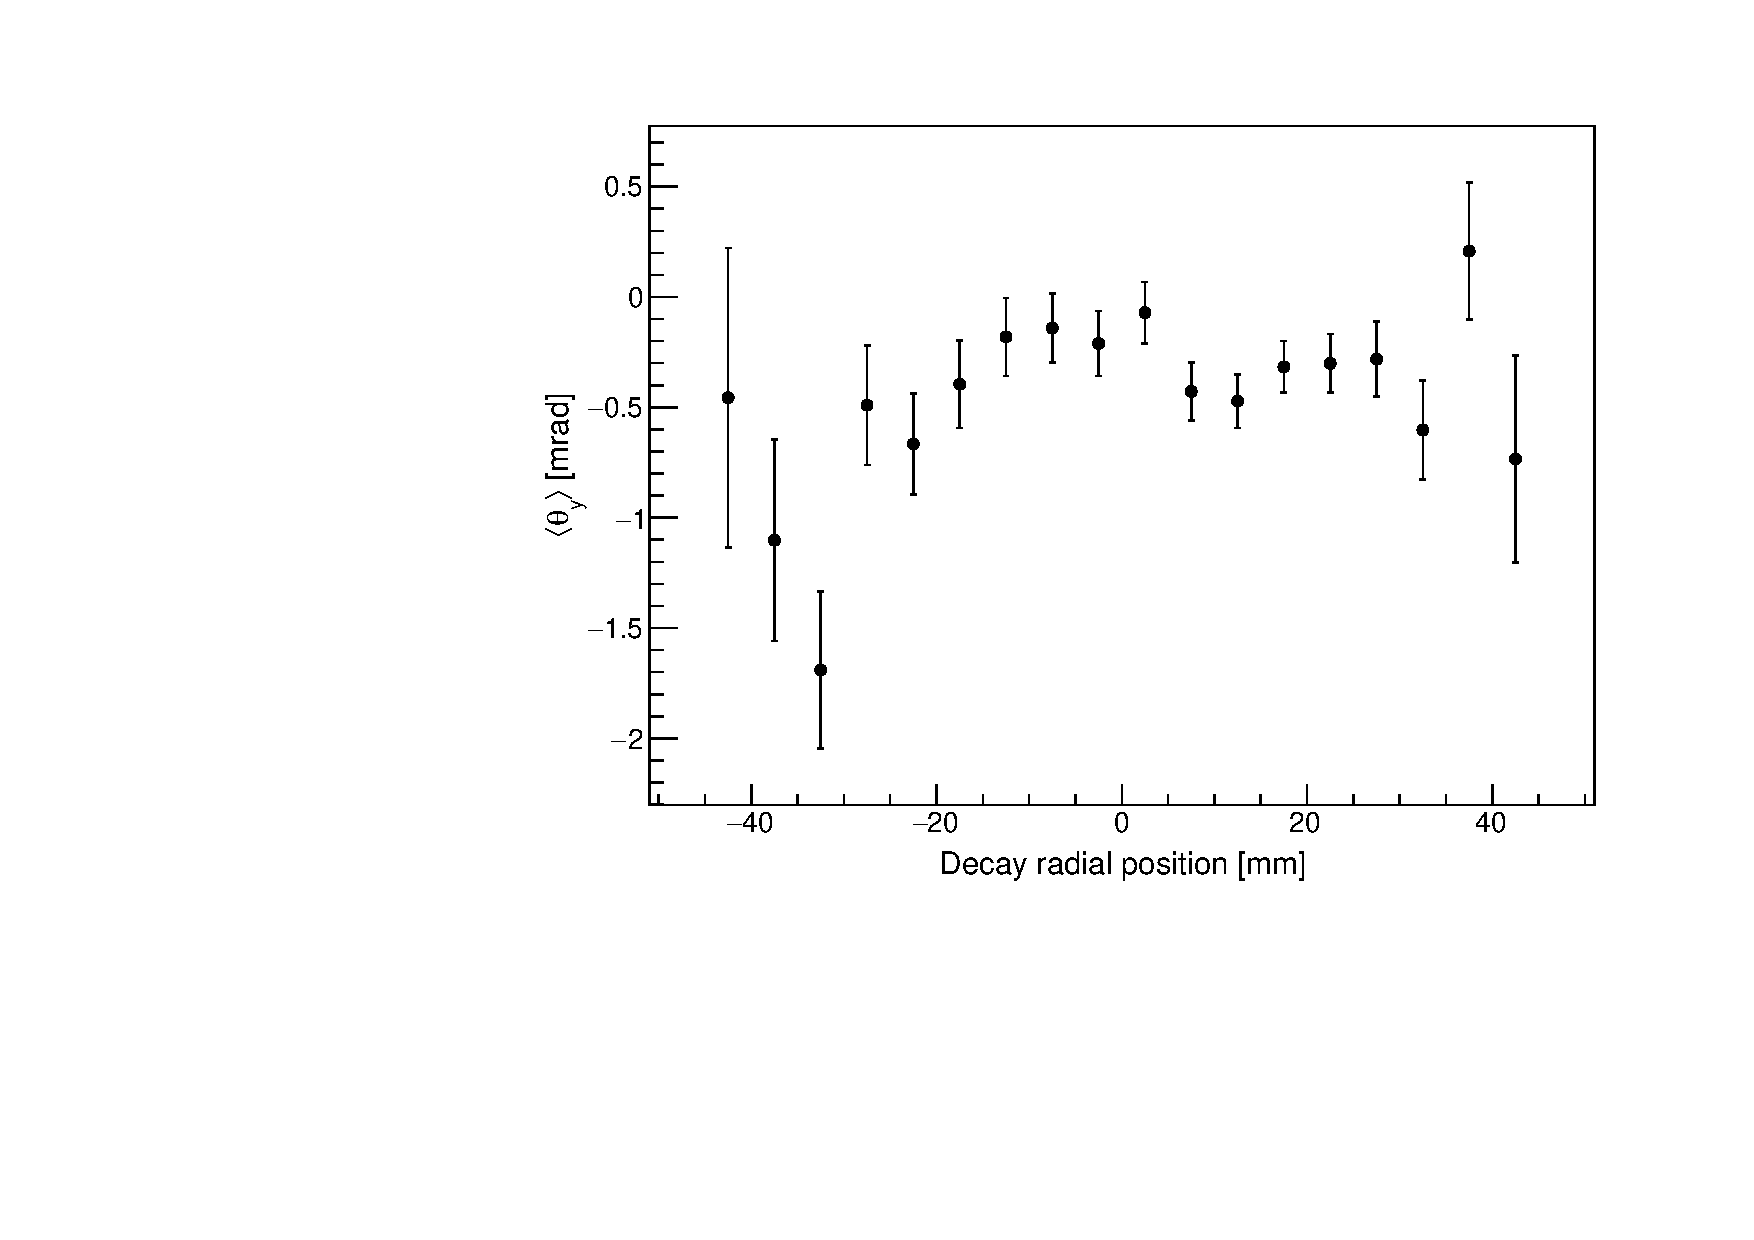
\includegraphics[trim={0 0 0 0},clip,width=.33\textwidth]{Images/Chapter5/S12_gr_thetaY_vs_R_tracks_0_3127_MeV.pdf}\label{subfig:ProfileR}}
\subfloat[Azimuthal.]{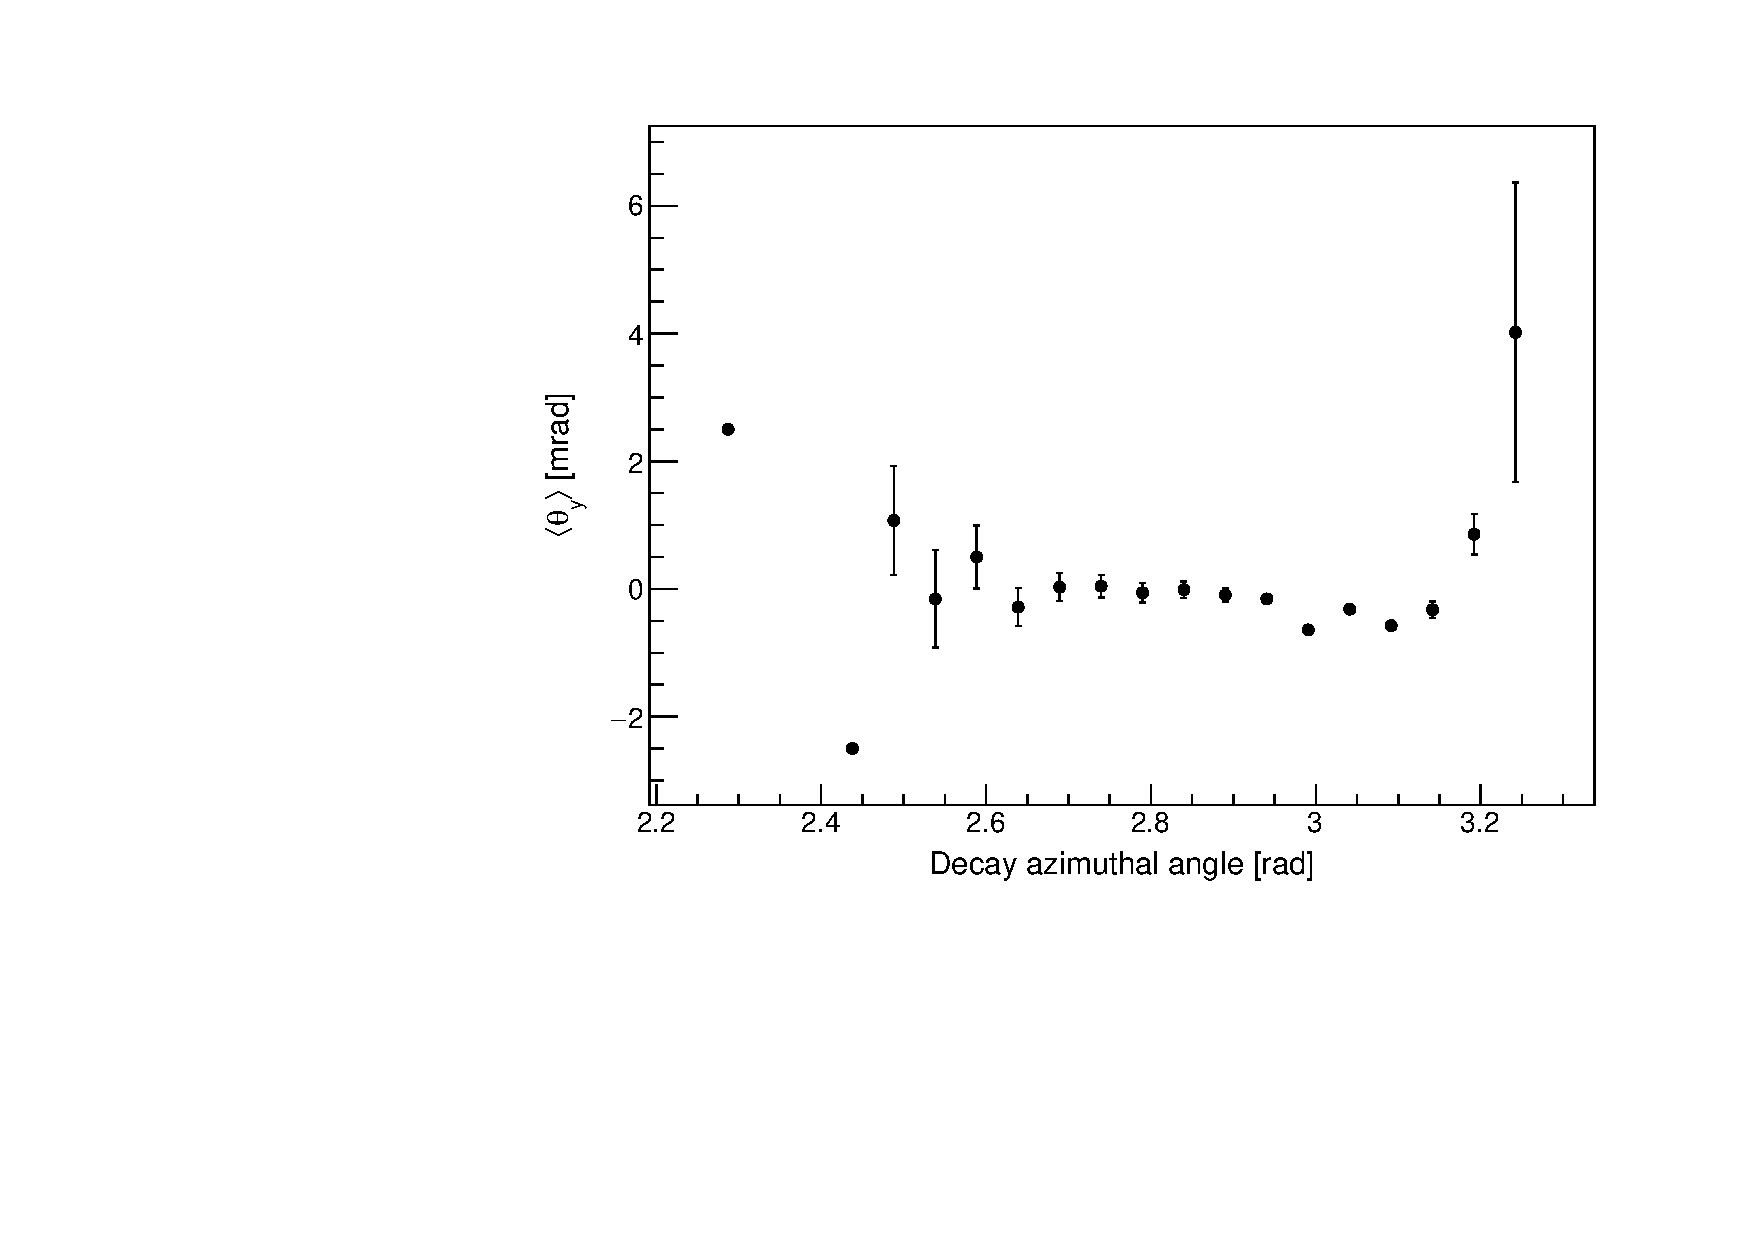
\includegraphics[trim={0 0 0 0},clip,width=.33\textwidth]{Images/Chapter5/S12_gr_thetaY_vs_Phi_tracks_0_3127_MeV.pdf}\label{subfig:ProfilePhi}}
\subfloat[Vertical.]{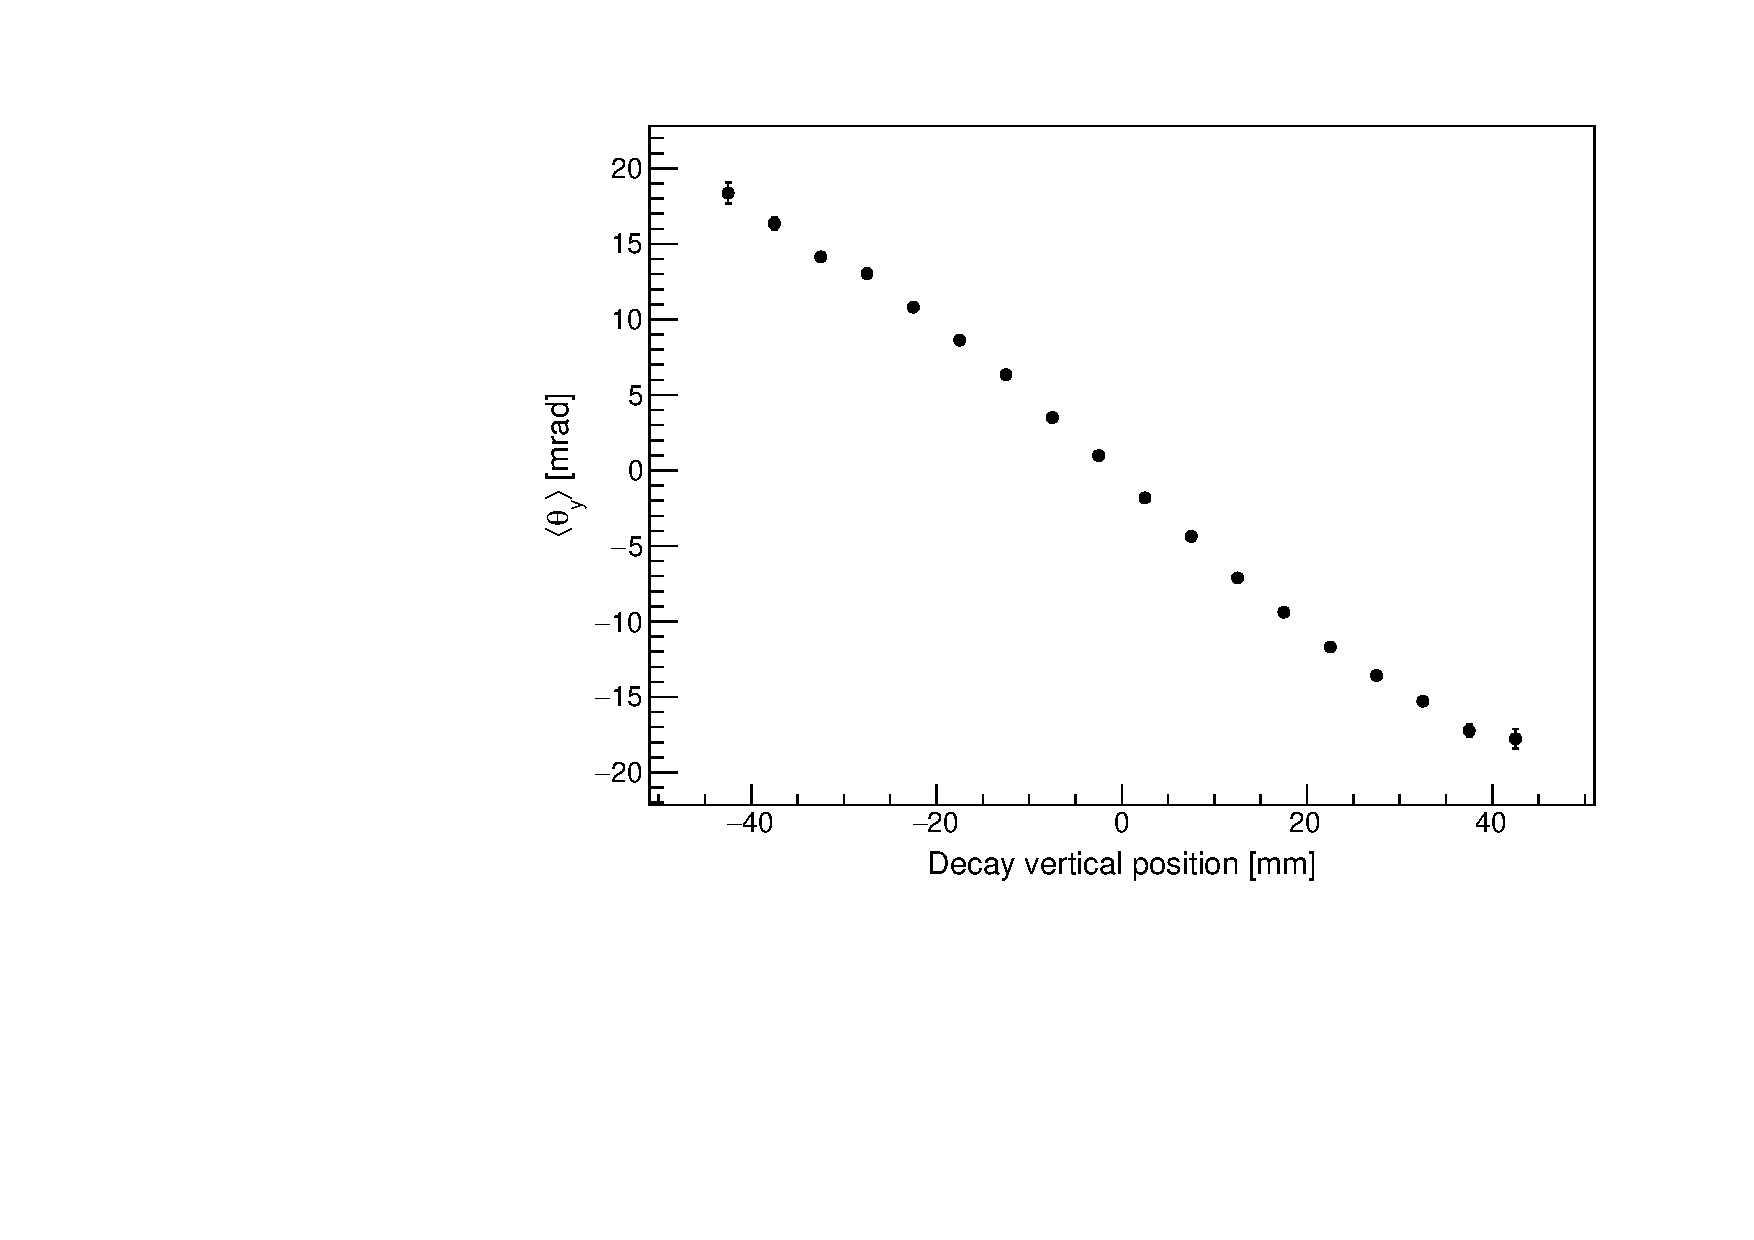
\includegraphics[trim={0 0 0 0},clip,width=.33\textwidth]{Images/Chapter5/S12_gr_thetaY_vs_Y_tracks_0_3127_MeV.pdf}\label{subfig:ProfileY}}
\caption{The distributions of accepted vertical angles in the radial, azimuthal, and vertical directions. A clear correlation is seen between $\theta_{y}$ and the vertical decay position. The azimuthal distributions presented in this figure are for station 12 only.}
\label{fig:AcceptanceCorrelations}
\end{figure} 

\begin{figure}[t!]
\centering{}
\subfloat[]{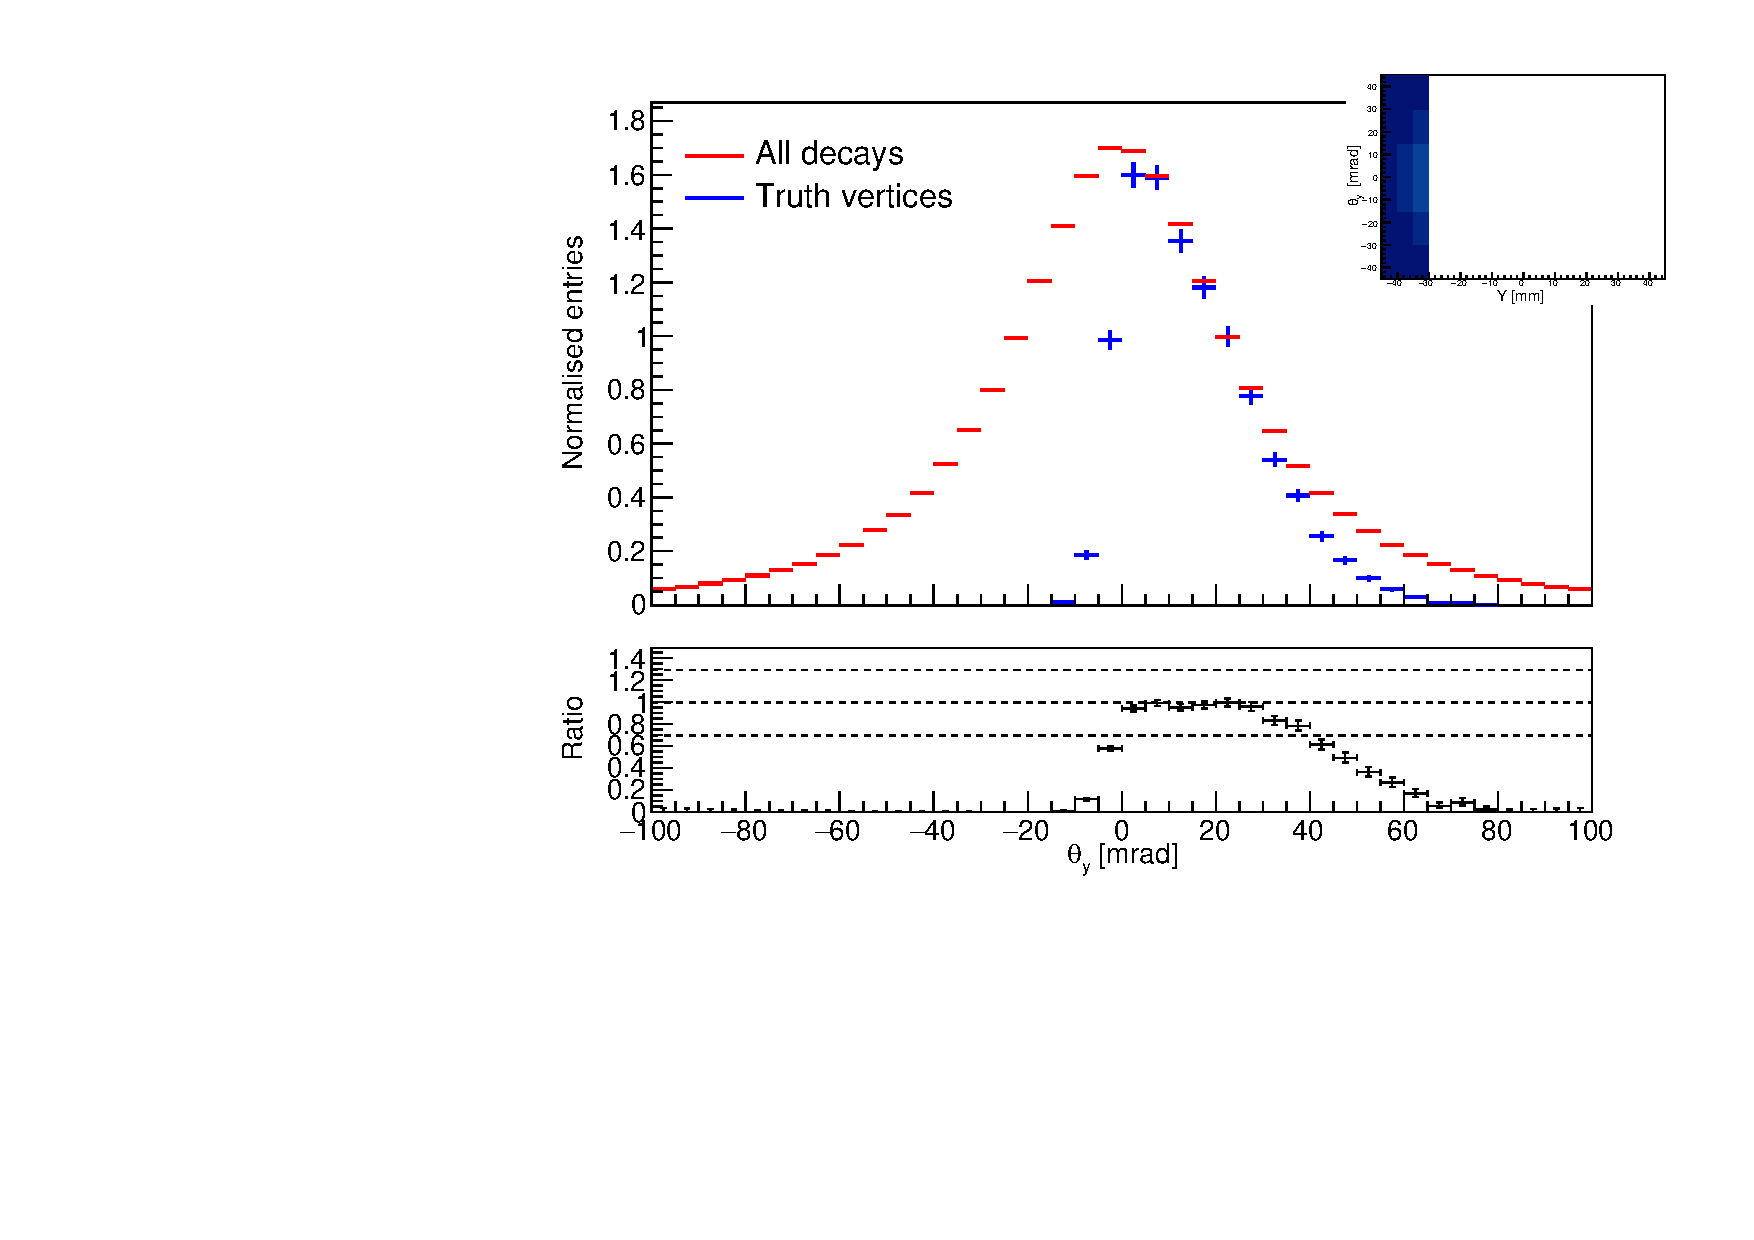
\includegraphics[trim={0 0 0 0},clip,width=.49\textwidth]{Images/Chapter5/S12S18_VerticalDecayAngleRatio_-45_-30.pdf}}
\subfloat[]{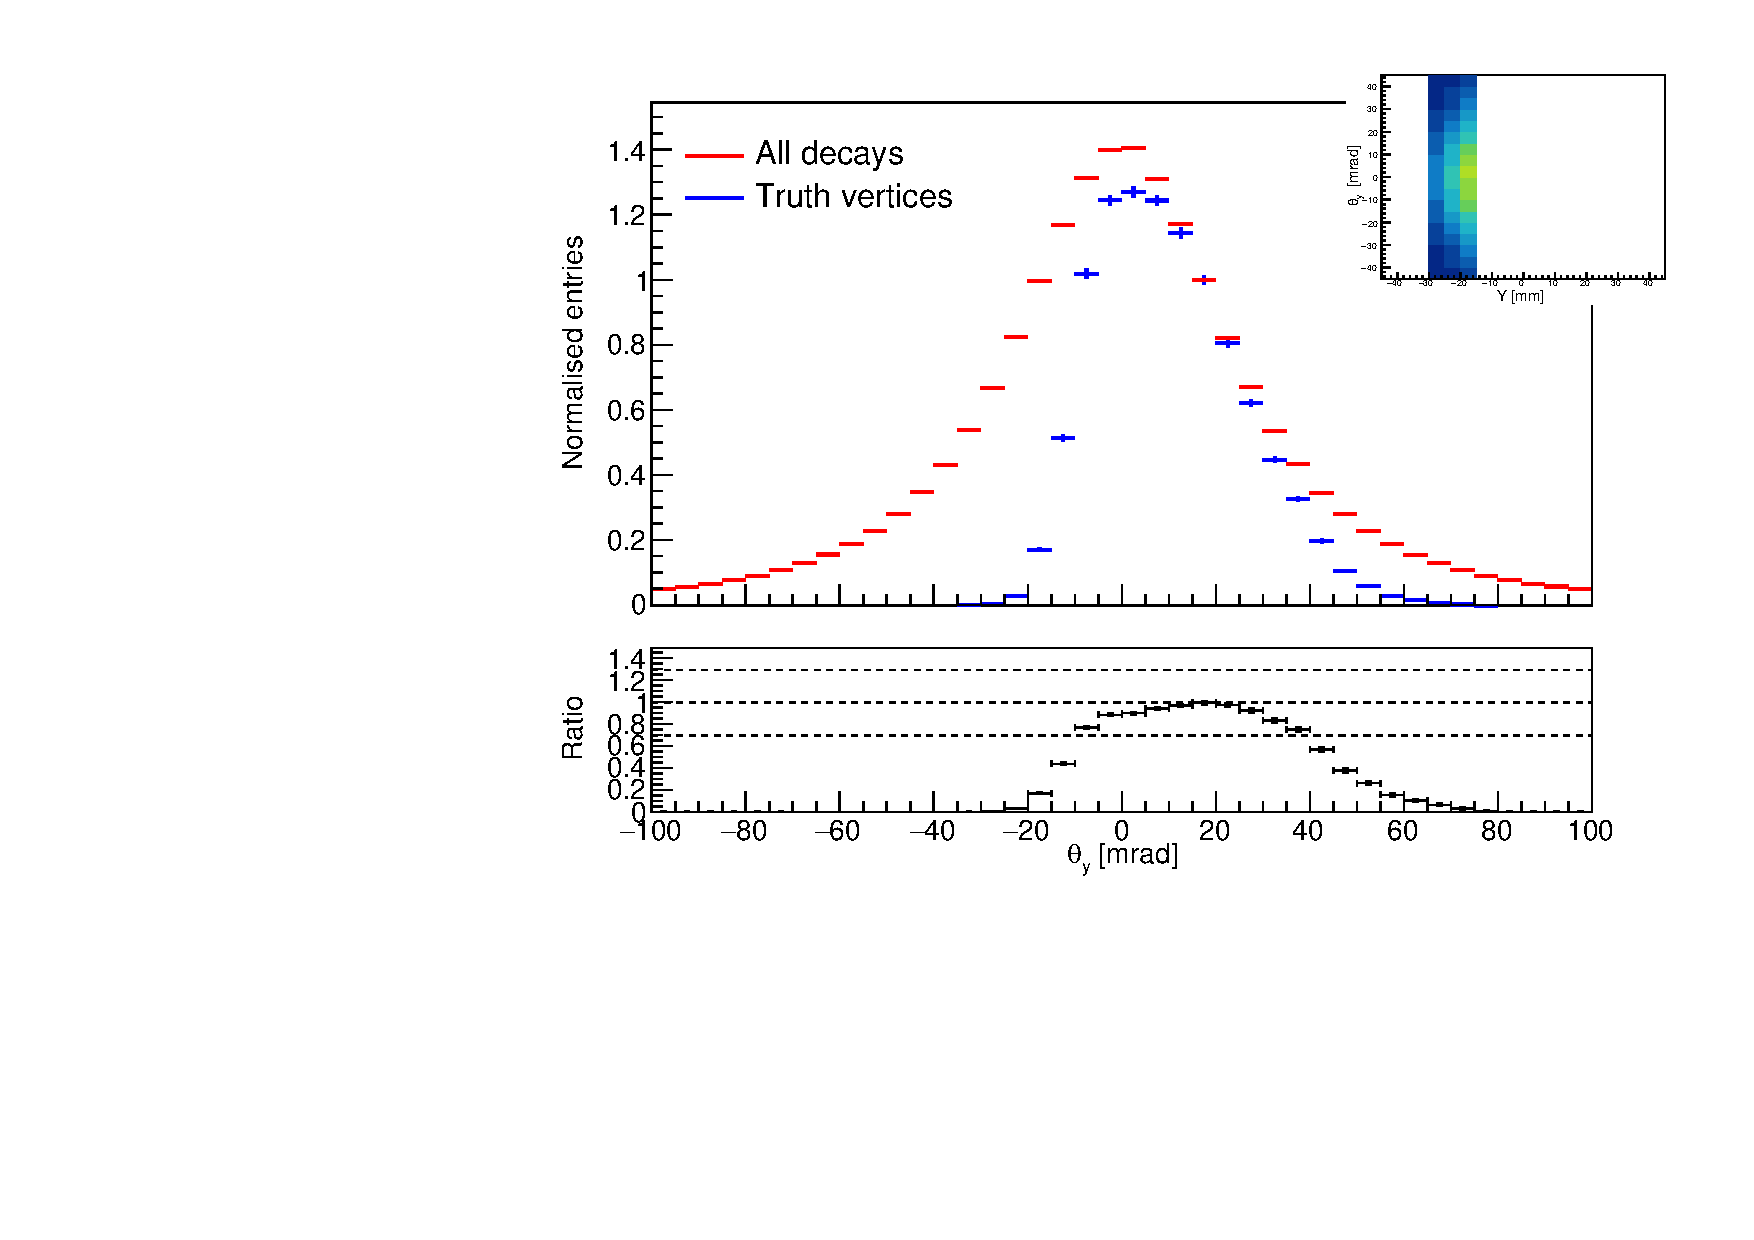
\includegraphics[trim={0 0 0 0},clip,width=.49\textwidth]{Images/Chapter5/S12S18_VerticalDecayAngleRatio_-30_-15.pdf}}
\hfill
\subfloat[]{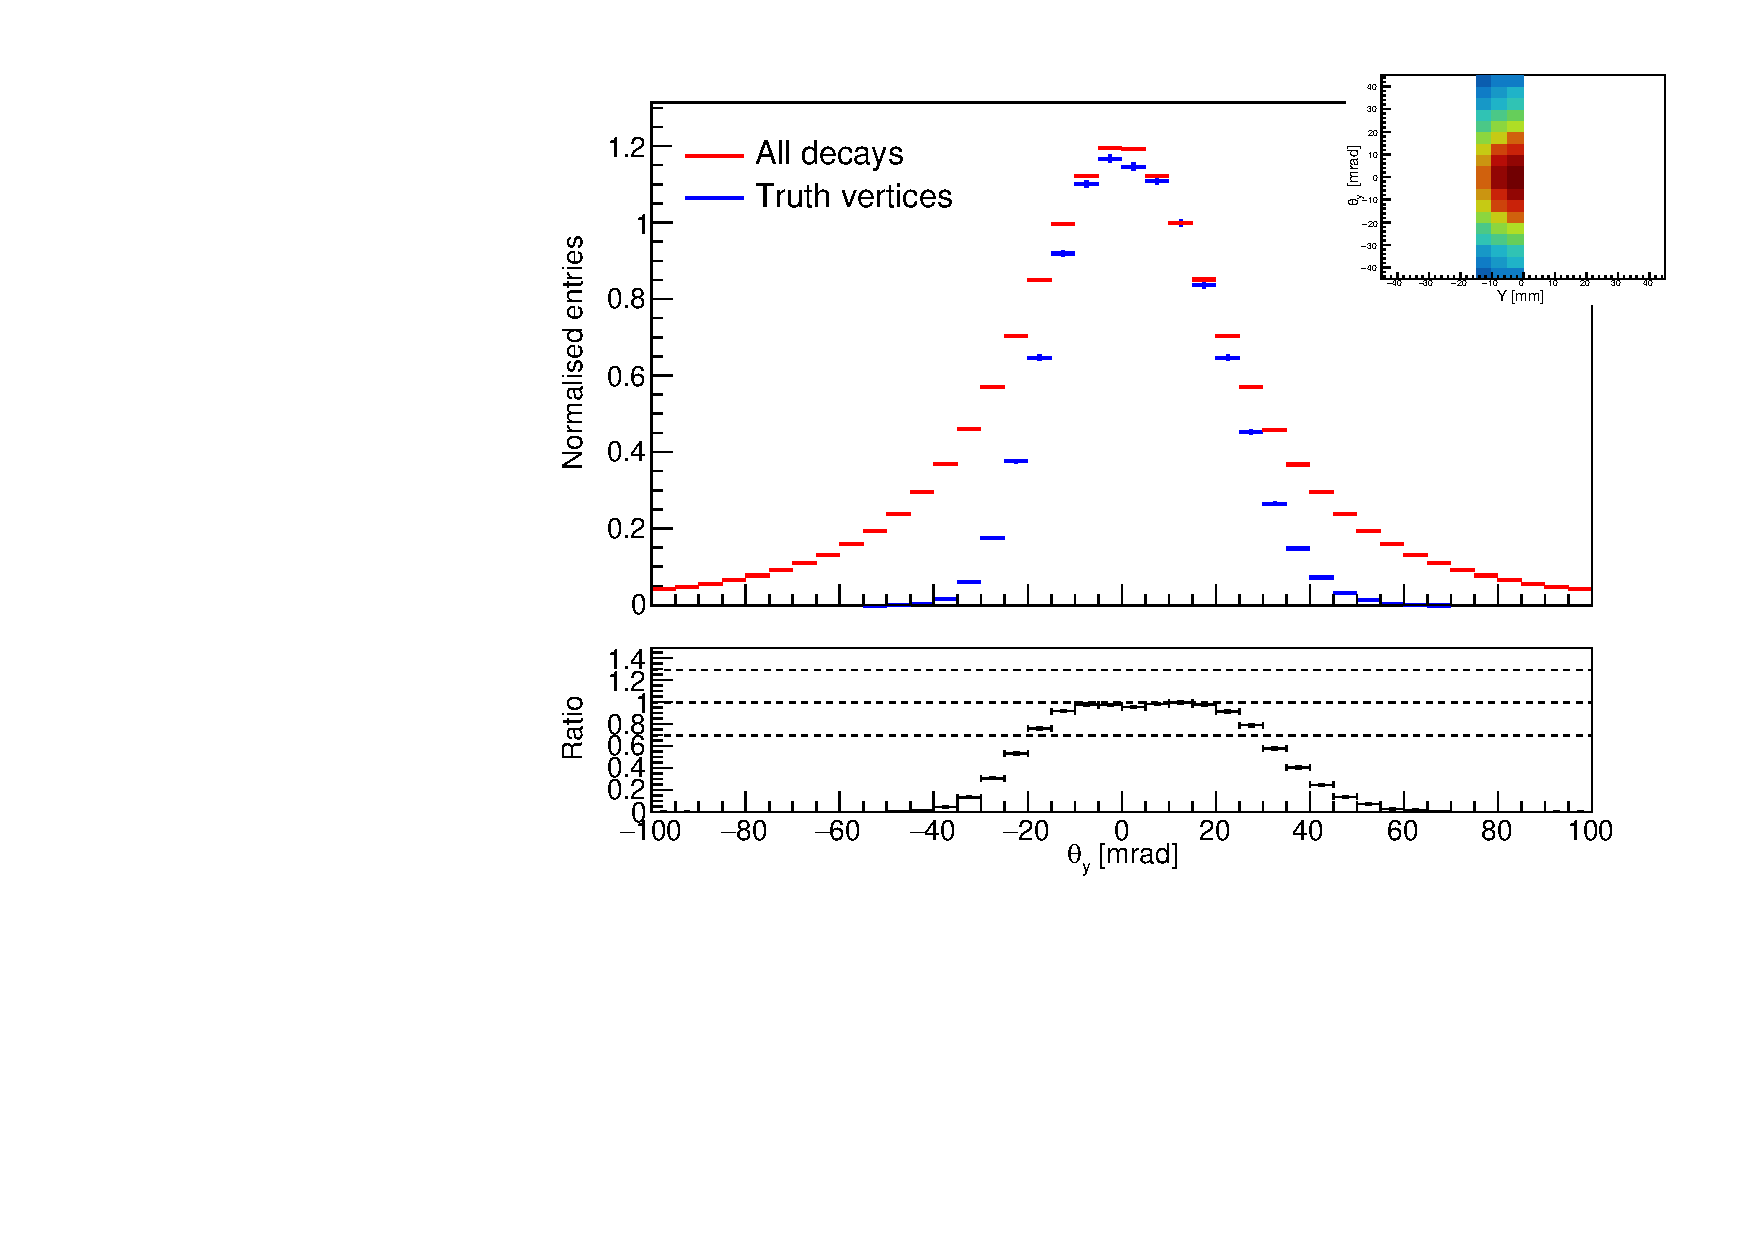
\includegraphics[trim={0 0 0 0},clip,width=.49\textwidth]{Images/Chapter5/S12S18_VerticalDecayAngleRatio_-15_0.pdf}}
\subfloat[]{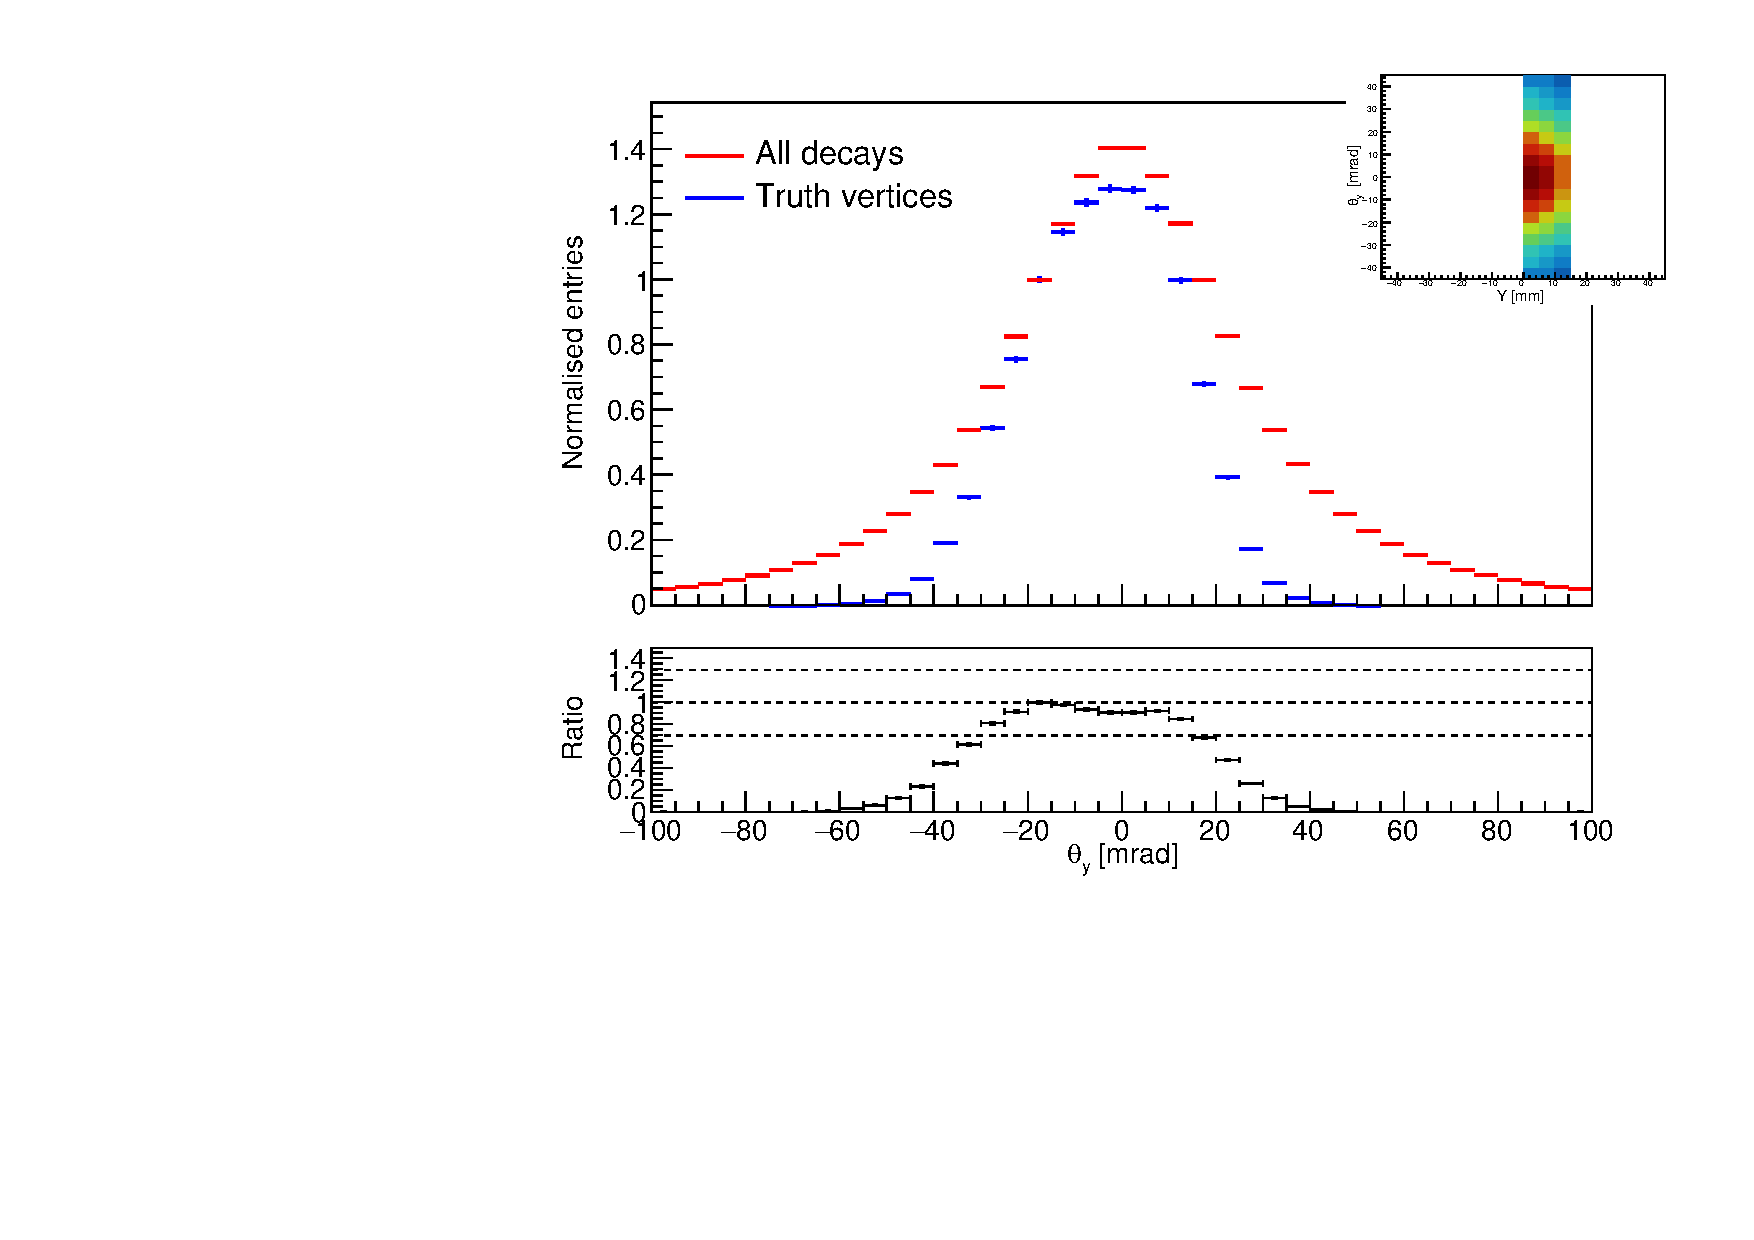
\includegraphics[trim={0 0 0 0},clip,width=.49\textwidth]{Images/Chapter5/S12S18_VerticalDecayAngleRatio_0_15.pdf}}
\hfill
\subfloat[]{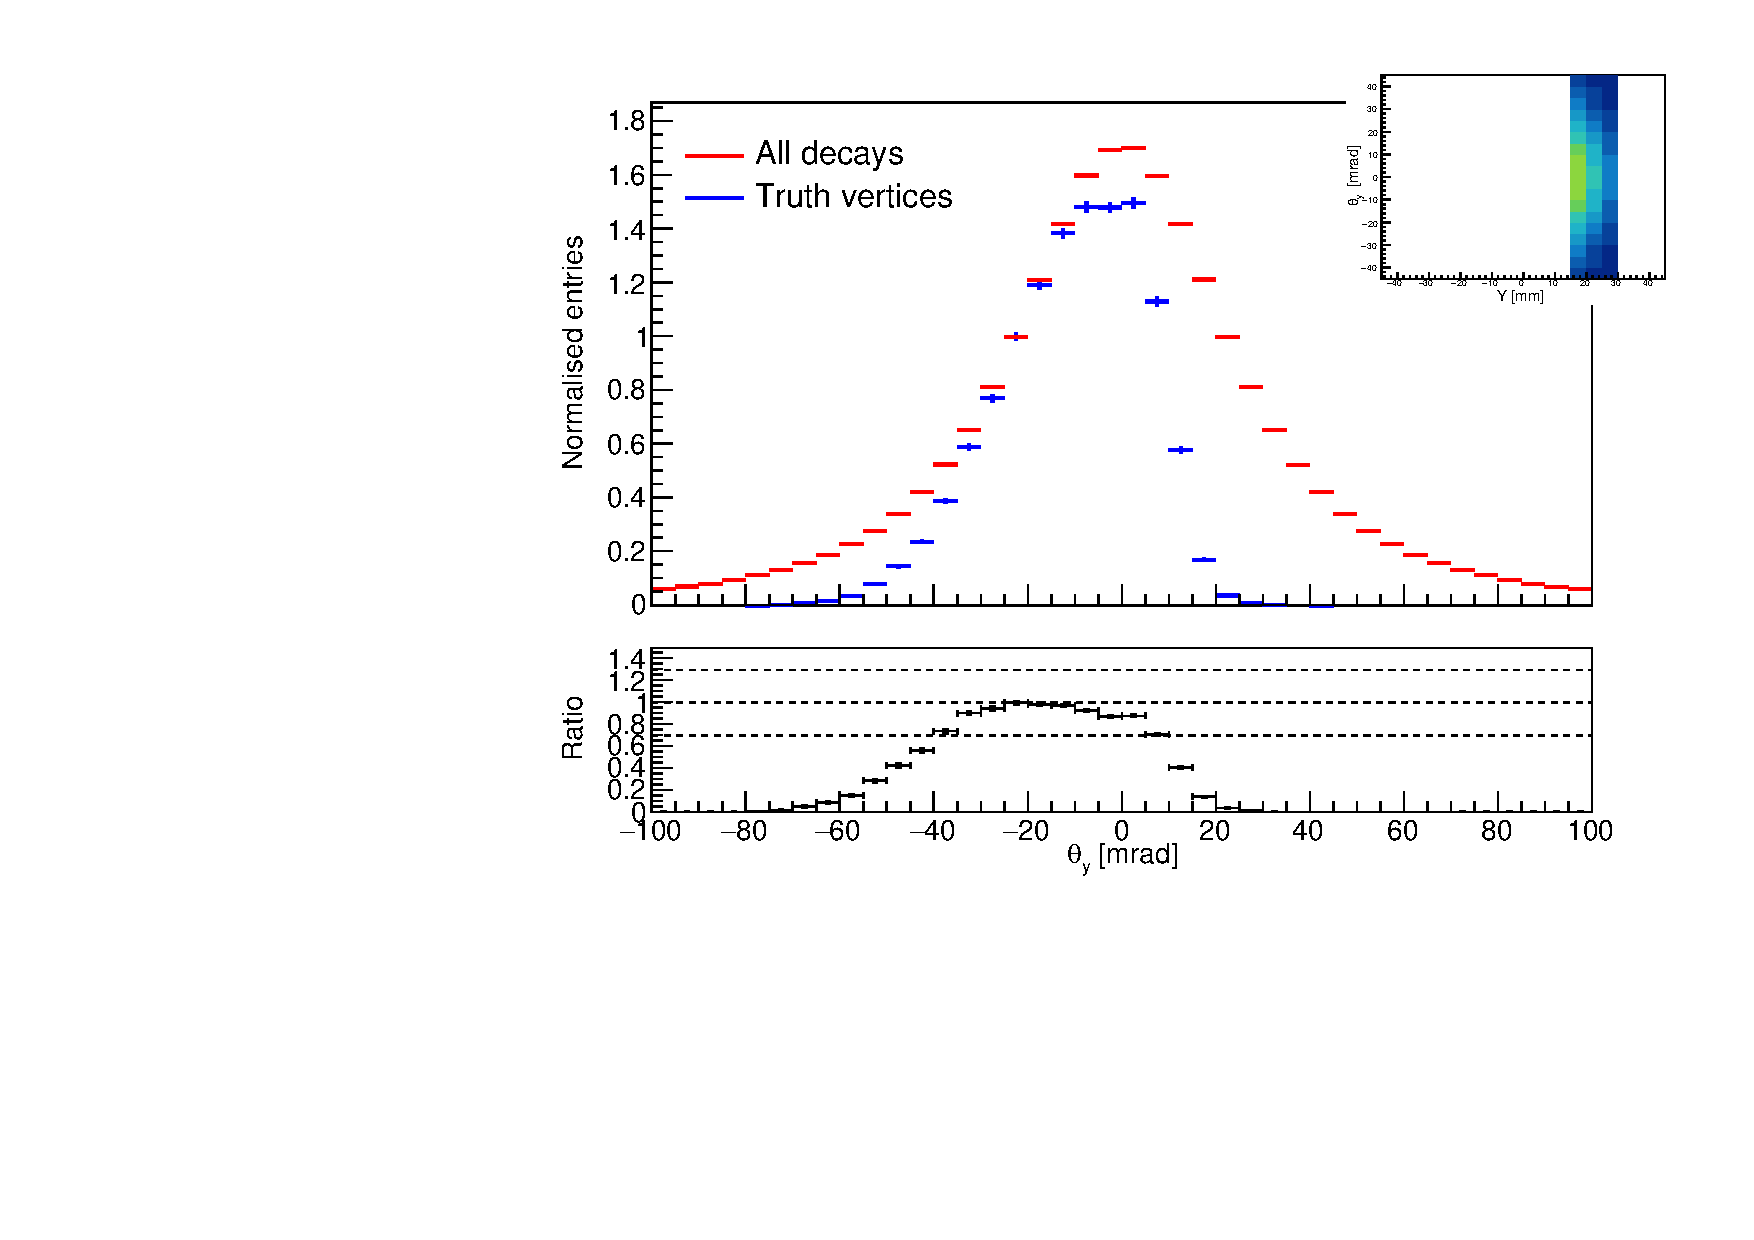
\includegraphics[trim={0 0 0 0},clip,width=.49\textwidth]{Images/Chapter5/S12S18_VerticalDecayAngleRatio_15_30.pdf}}
\subfloat[]{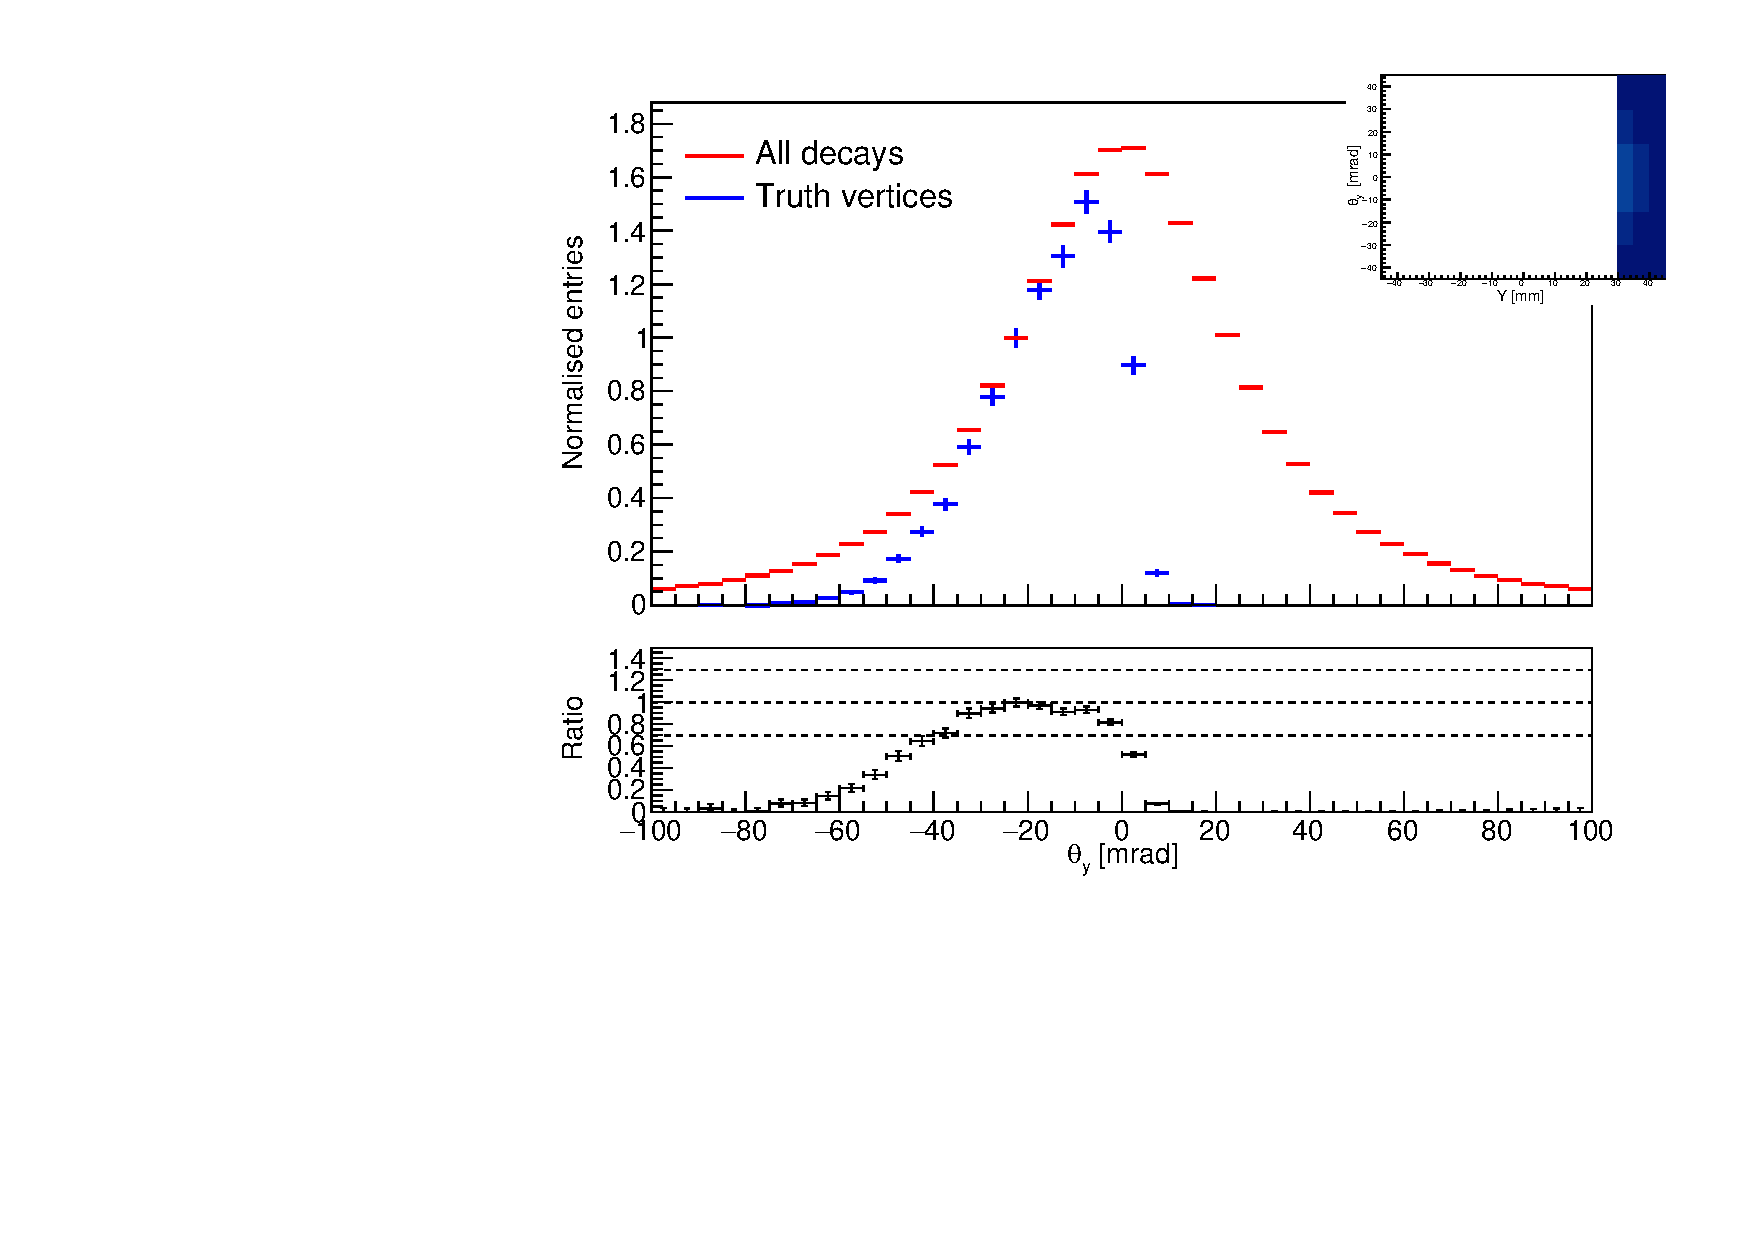
\includegraphics[trim={0 0 0 0},clip,width=.49\textwidth]{Images/Chapter5/S12S18_VerticalDecayAngleRatio_30_45.pdf}}
\caption{$\theta_{y}$ acceptance ratios in $y$ intervals of \SI{15}{\milli\metre}, indicated by secondary two-dimensional histograms. Positrons originating from the bottom of the storage region must carry a positive vertical component of momentum to be accepted by the straw trackers, and vice versa, resulting in negative correlation between $\theta_{y}$ and $y$. Histograms are formed from a Monte Carlo sample where vertices are a subset of decays, the one-dimensional distributions are normalised to their maximum ratio, and tracker stations are combined.} 
\label{fig:1DAcceptanceRatios}
\end{figure} 

The vertical angle acceptance of the straw trackers is three-dimensional, with varying acceptance of $\theta_{y}$ in the radial, azimuthal, and vertical axes. Distributions of $\theta_{y}$ in each of these three dimensions are given in Figure \ref{fig:AcceptanceCorrelations}, showing both two-dimensional histograms and their corresponding one-dimensional $x$-axis profiles. Little correlation is observed between $\theta_{y}$ and the radial decay position or azimuthal decay angle, while there is a clear negative correlation between $\theta_{y}$ and the vertical decay position, $y$, as shown by Figure \ref{subfig:ProfileY}. For this reason, it was decided that only the vertical component of $\theta_{y}$ acceptance need be considered for the study presented in this section.





% \begin{figure}[t!]
% \centering{}
% \subfloat[]{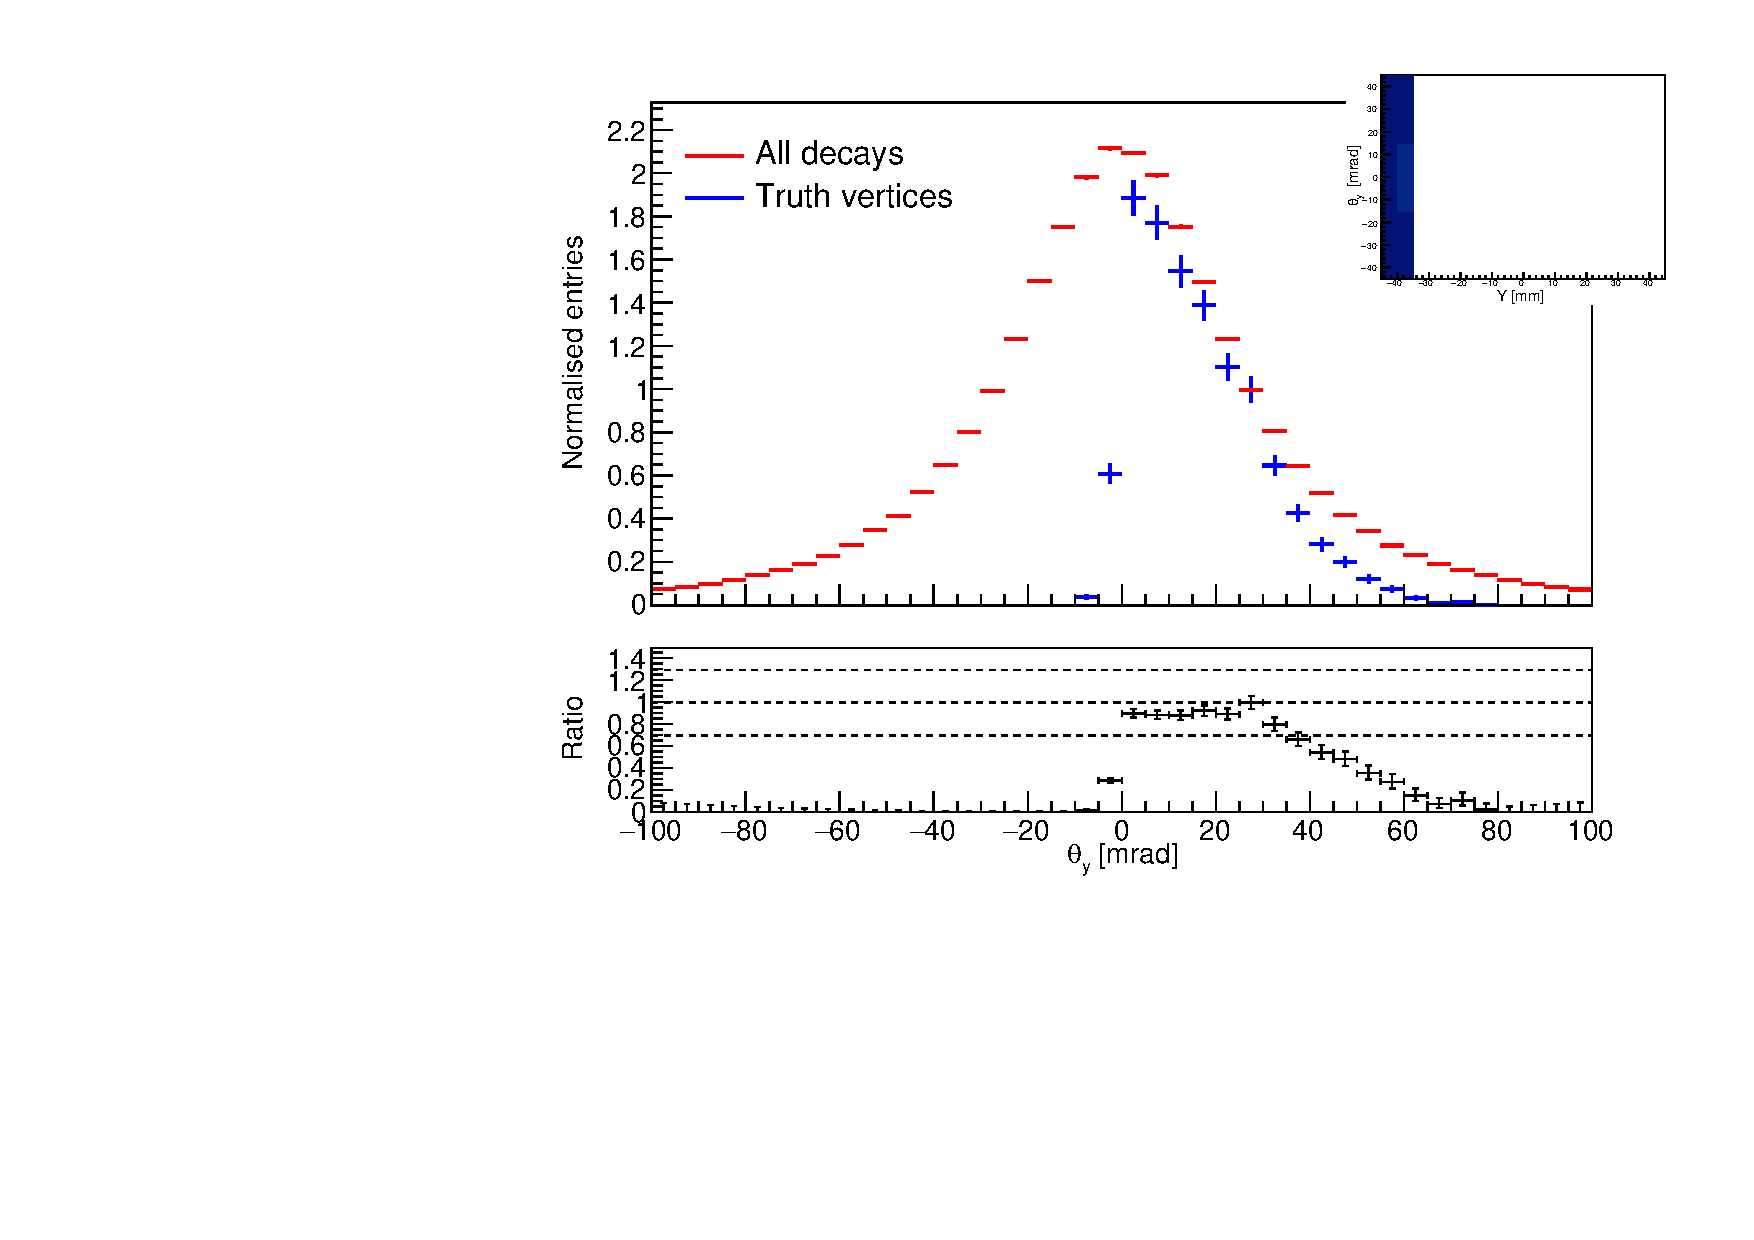
\includegraphics[trim={0 0 0 0},clip,width=.33\textwidth]{Images/Chapter5/S12S18_VerticalDecayAngleRatio_-45_-35.pdf}}
% \subfloat[]{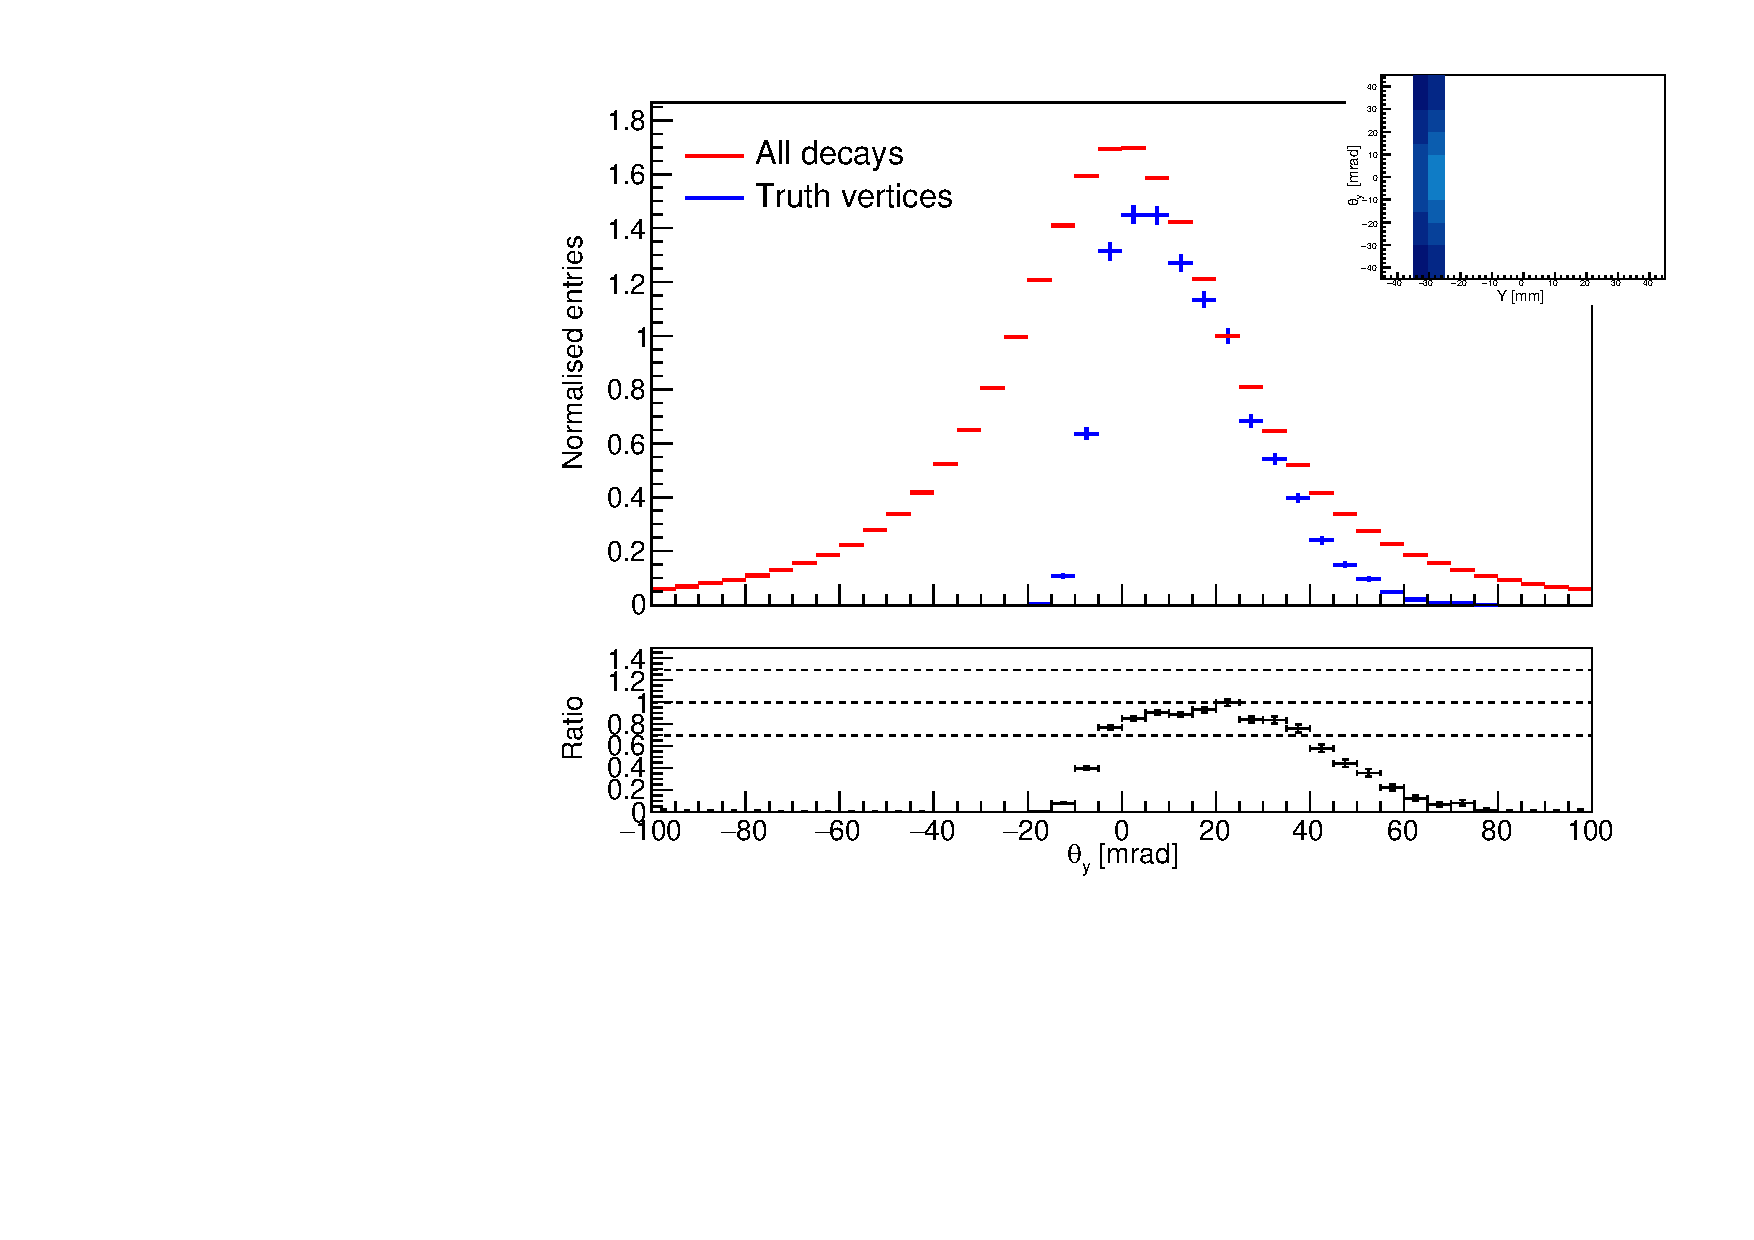
\includegraphics[trim={0 0 0 0},clip,width=.33\textwidth]{Images/Chapter5/S12S18_VerticalDecayAngleRatio_-35_-25.pdf}}
% \subfloat[]{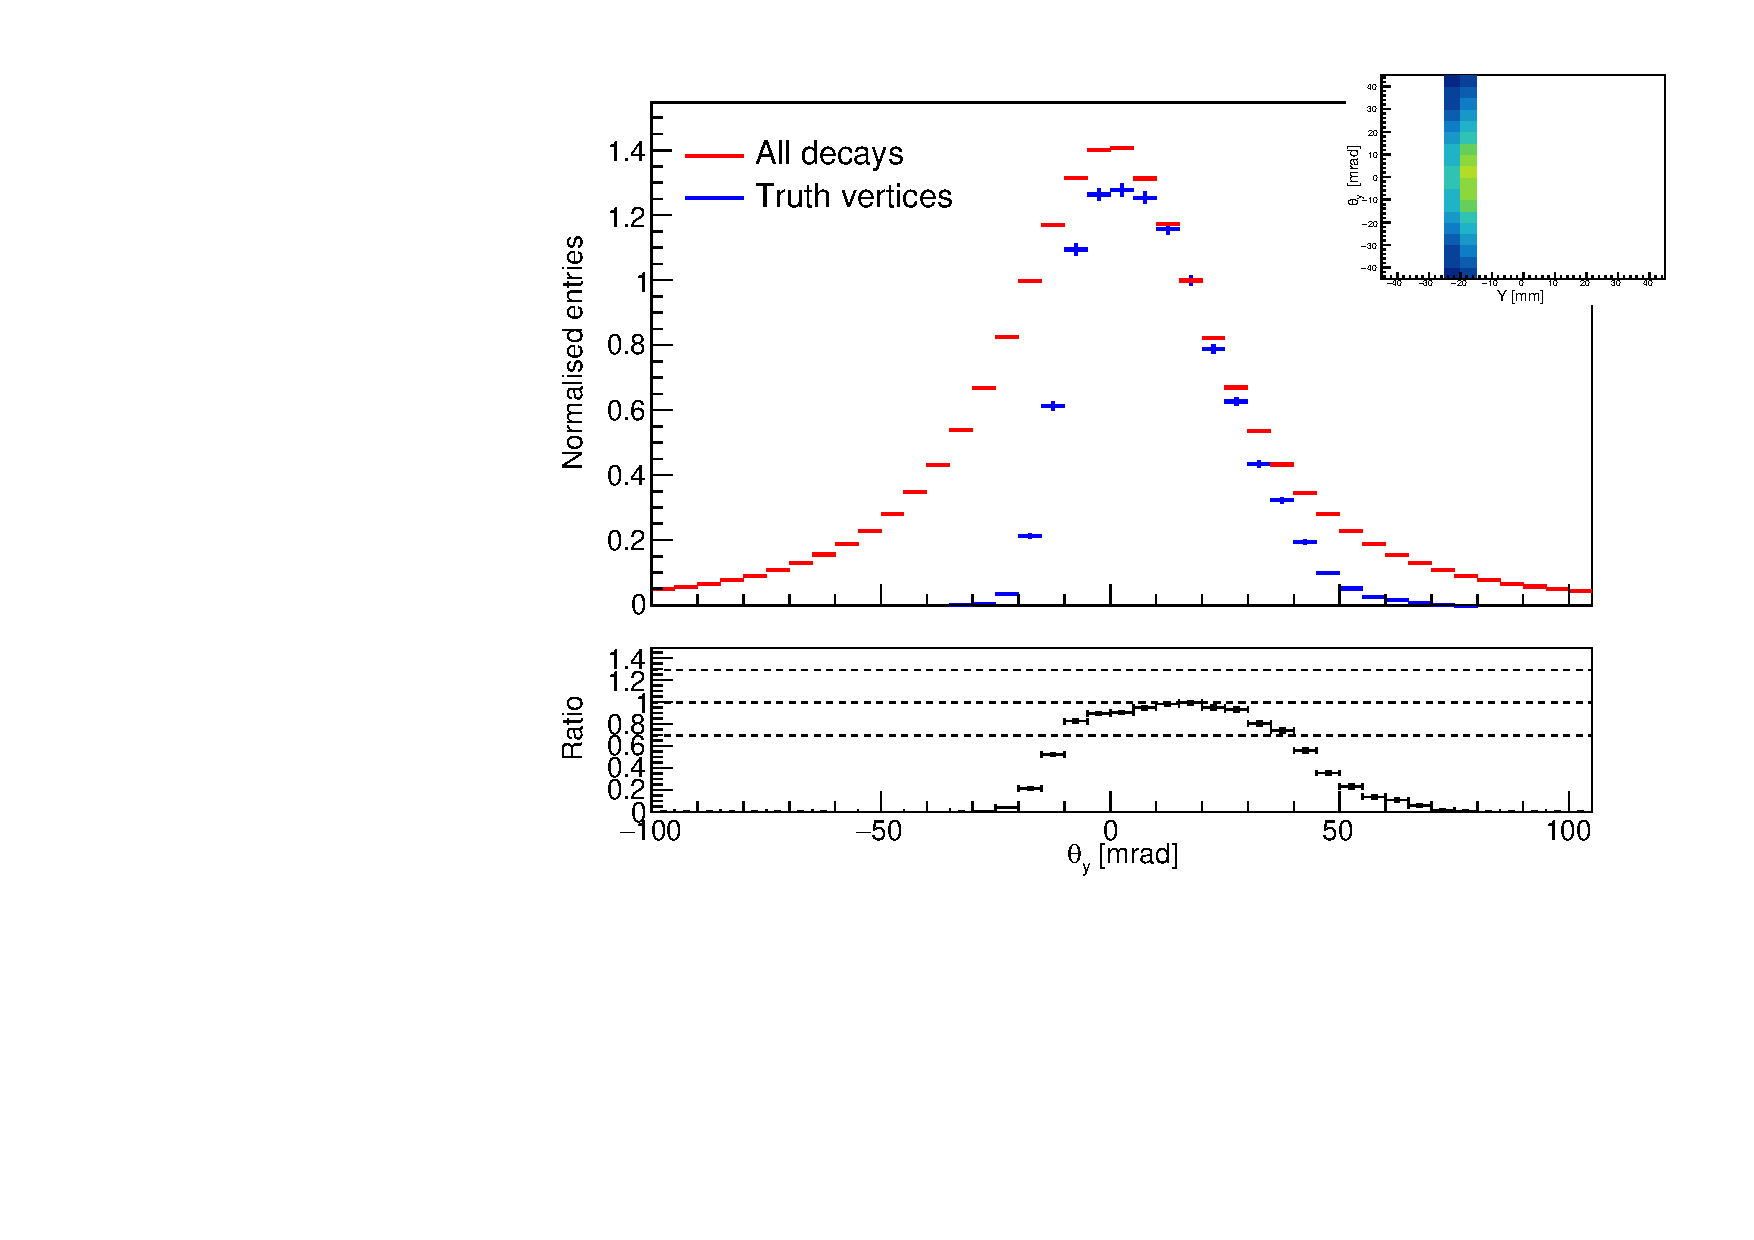
\includegraphics[trim={0 0 0 0},clip,width=.33\textwidth]{Images/Chapter5/S12S18_VerticalDecayAngleRatio_-25_-15.pdf}}
% \hfill
% \subfloat[]{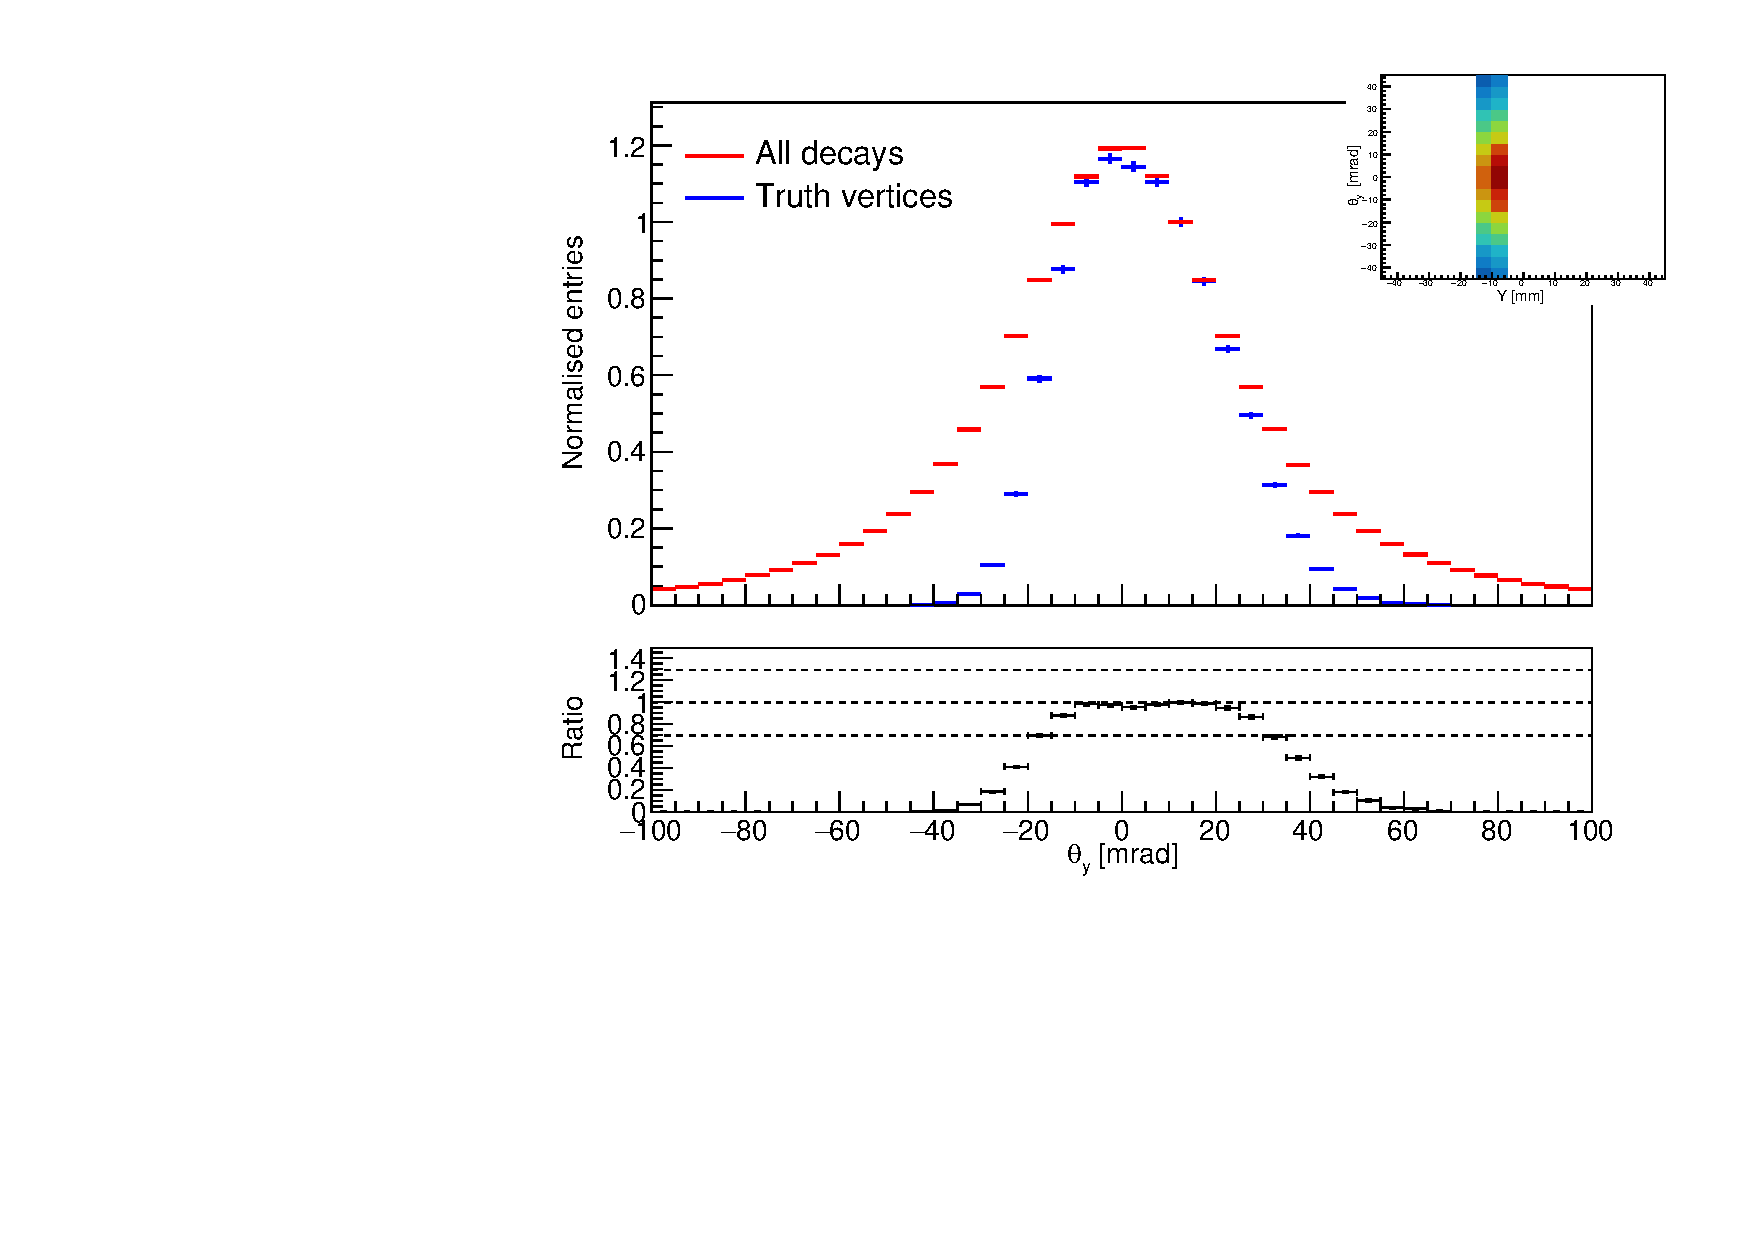
\includegraphics[trim={0 0 0 0},clip,width=.33\textwidth]{Images/Chapter5/S12S18_VerticalDecayAngleRatio_-15_-5.pdf}}
% \subfloat[]{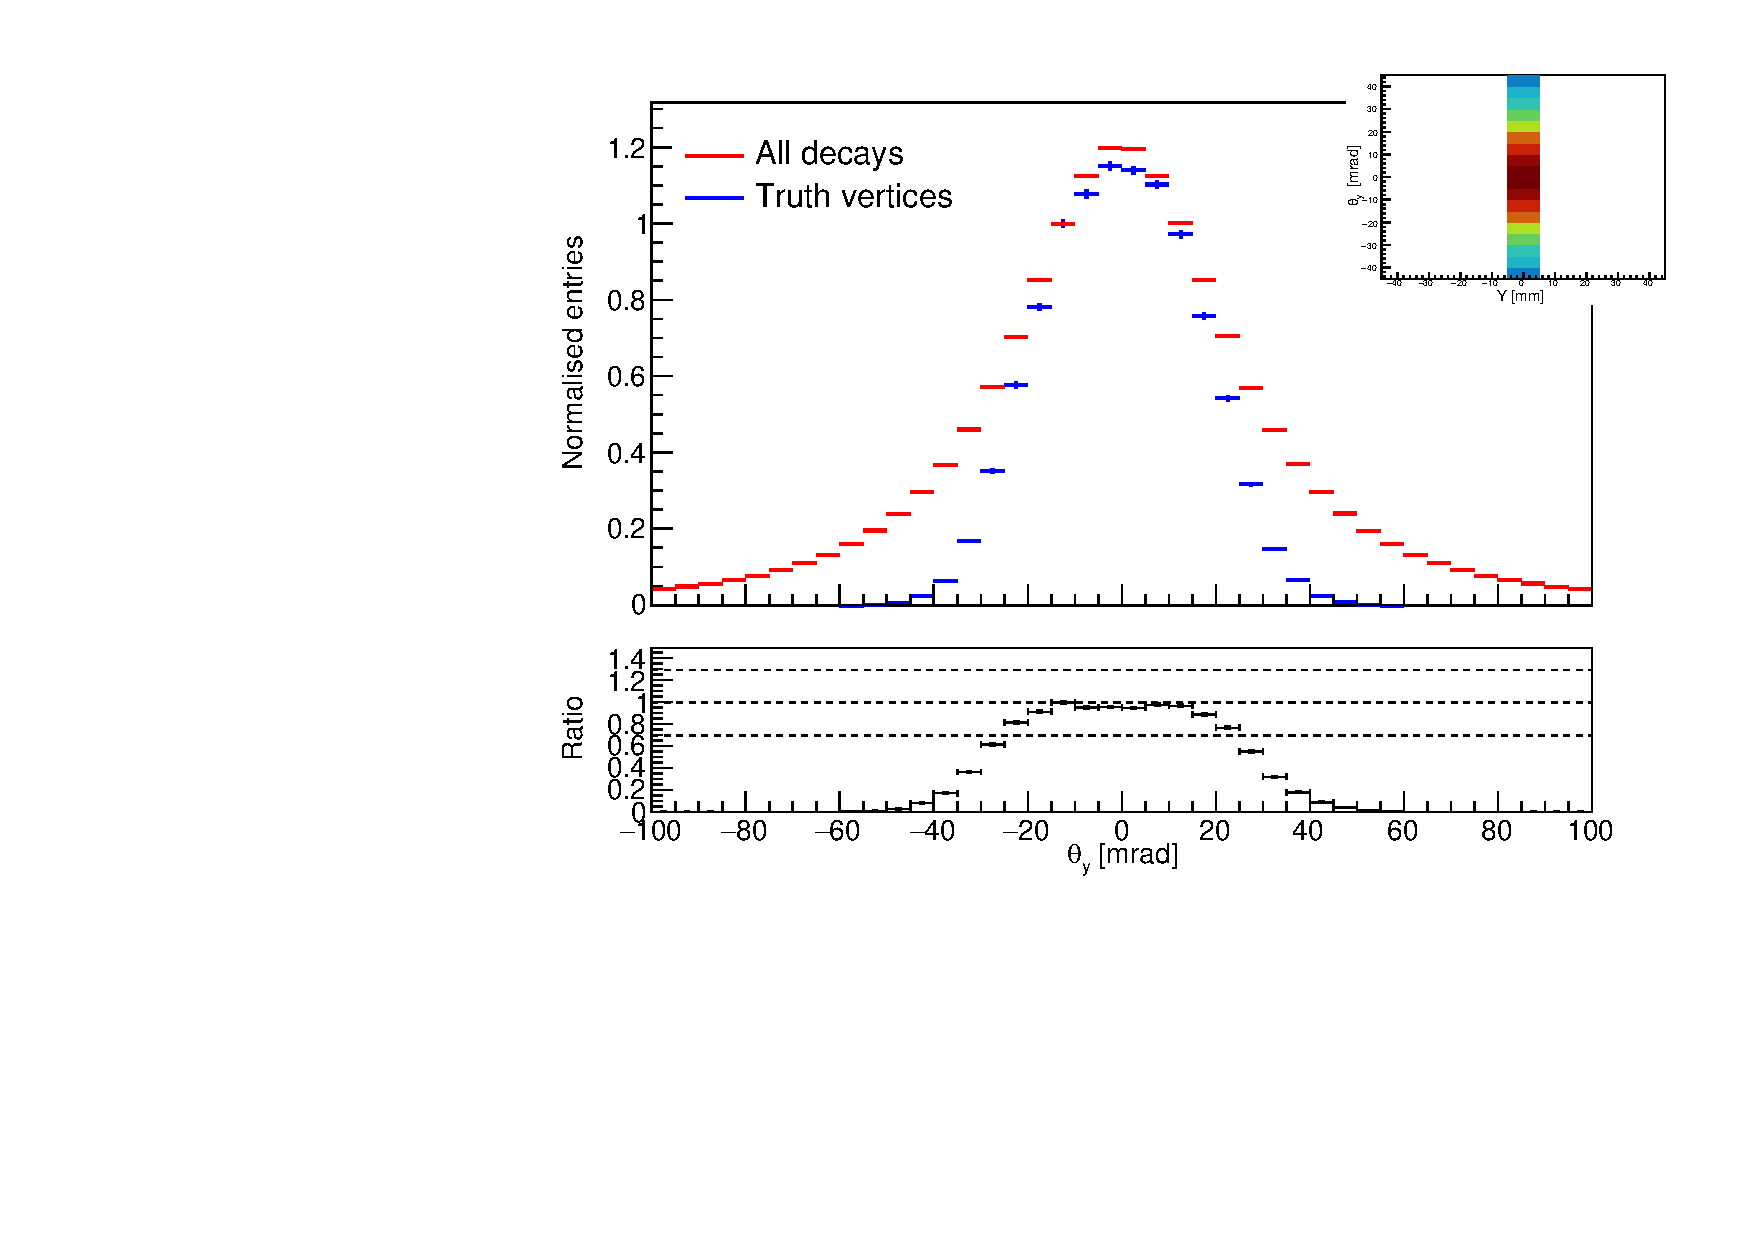
\includegraphics[trim={0 0 0 0},clip,width=.33\textwidth]{Images/Chapter5/S12S18_VerticalDecayAngleRatio_-5_5.pdf}}
% \subfloat[]{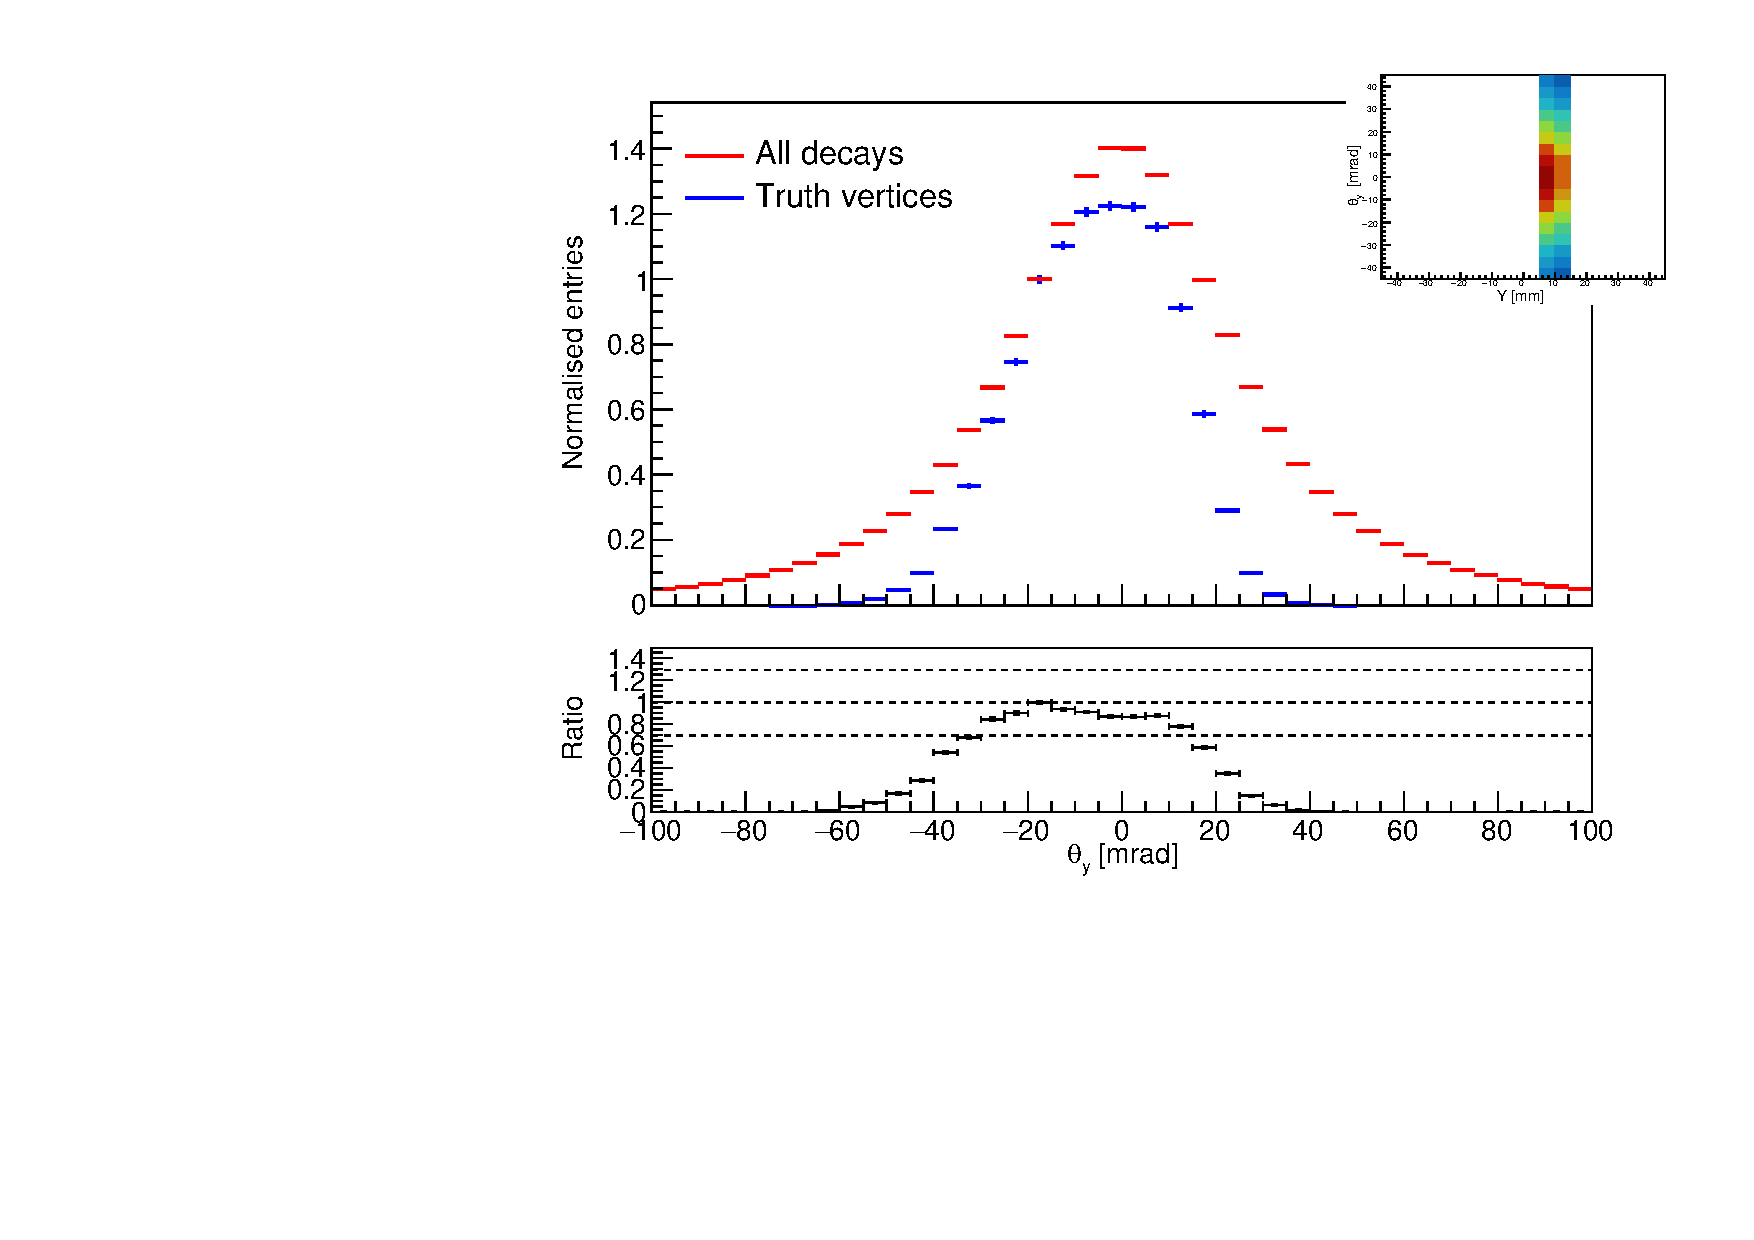
\includegraphics[trim={0 0 0 0},clip,width=.33\textwidth]{Images/Chapter5/S12S18_VerticalDecayAngleRatio_5_15.pdf}}
% \hfill
% \subfloat[]{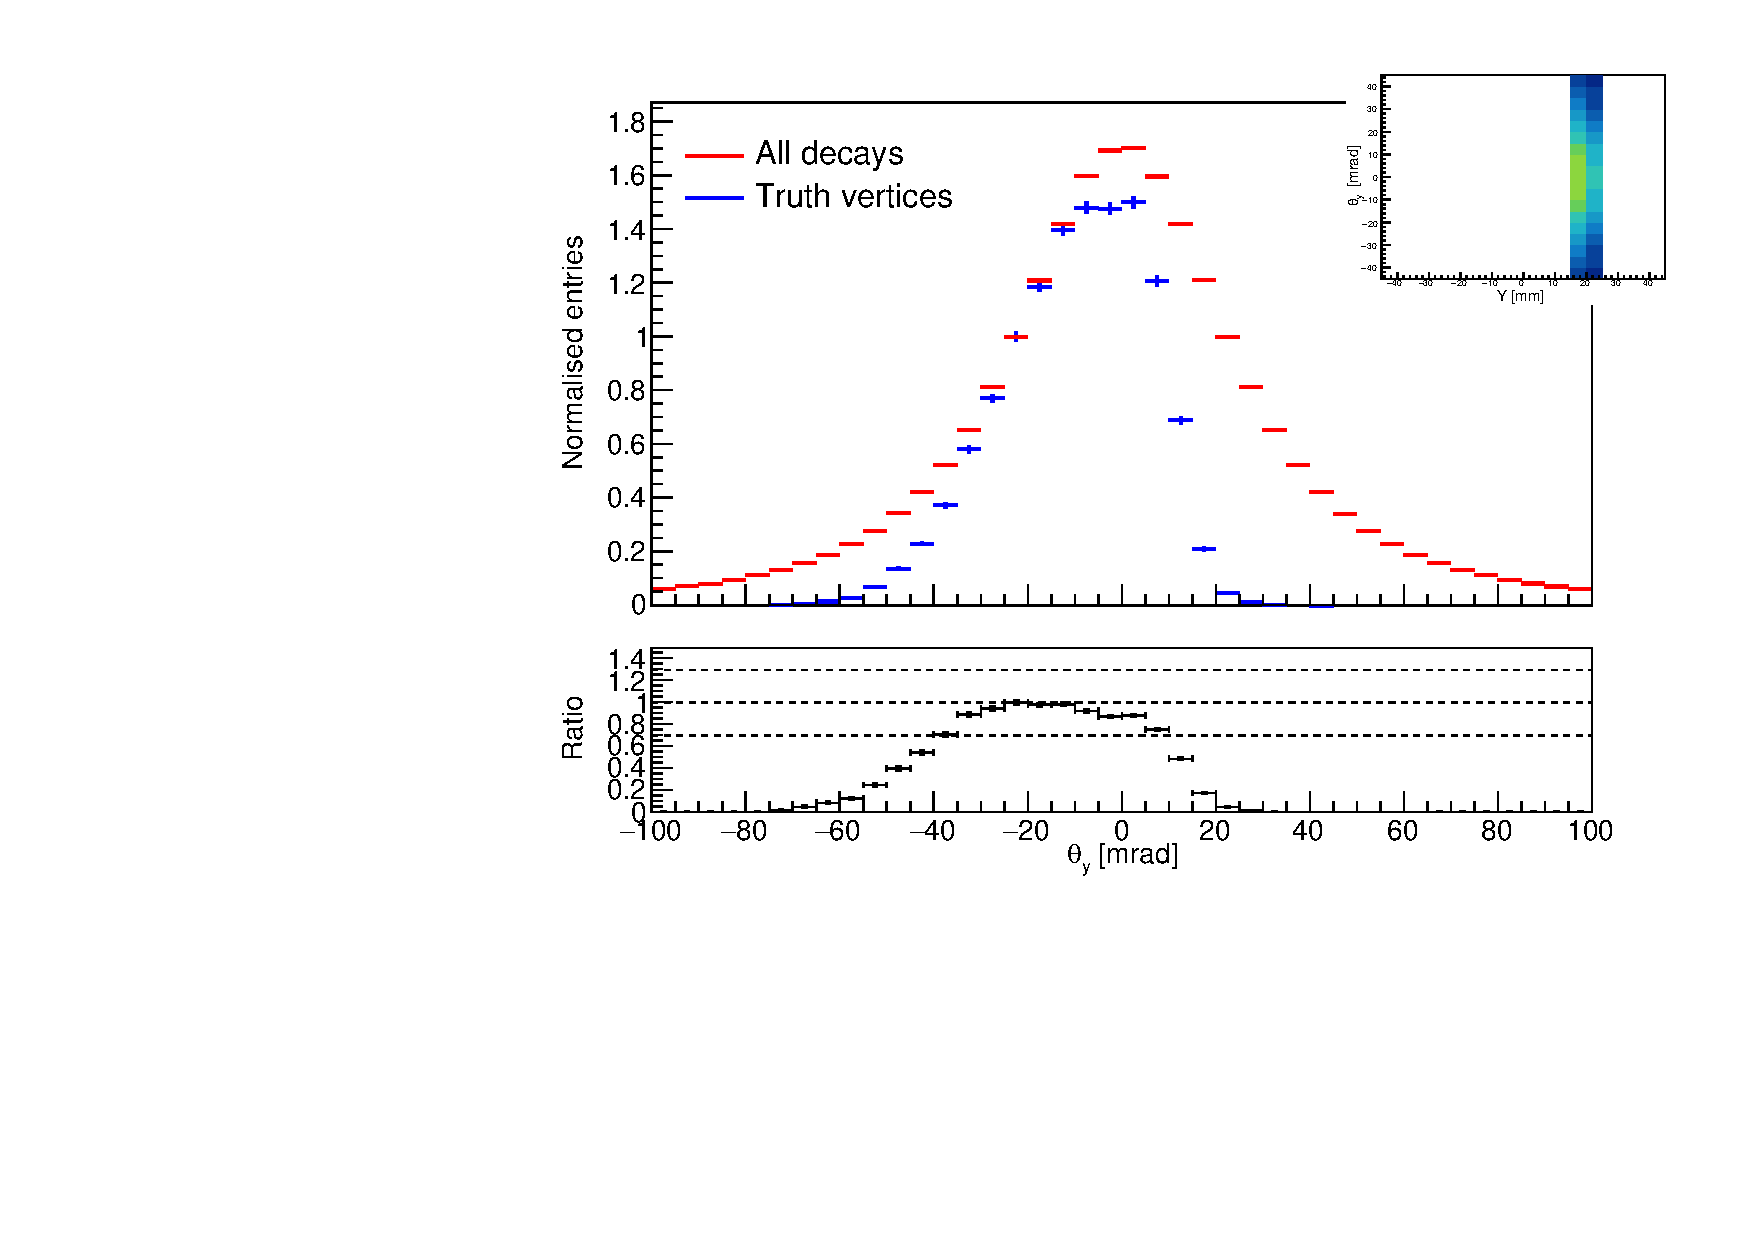
\includegraphics[trim={0 0 0 0},clip,width=.33\textwidth]{Images/Chapter5/S12S18_VerticalDecayAngleRatio_15_25.pdf}}
% \subfloat[]{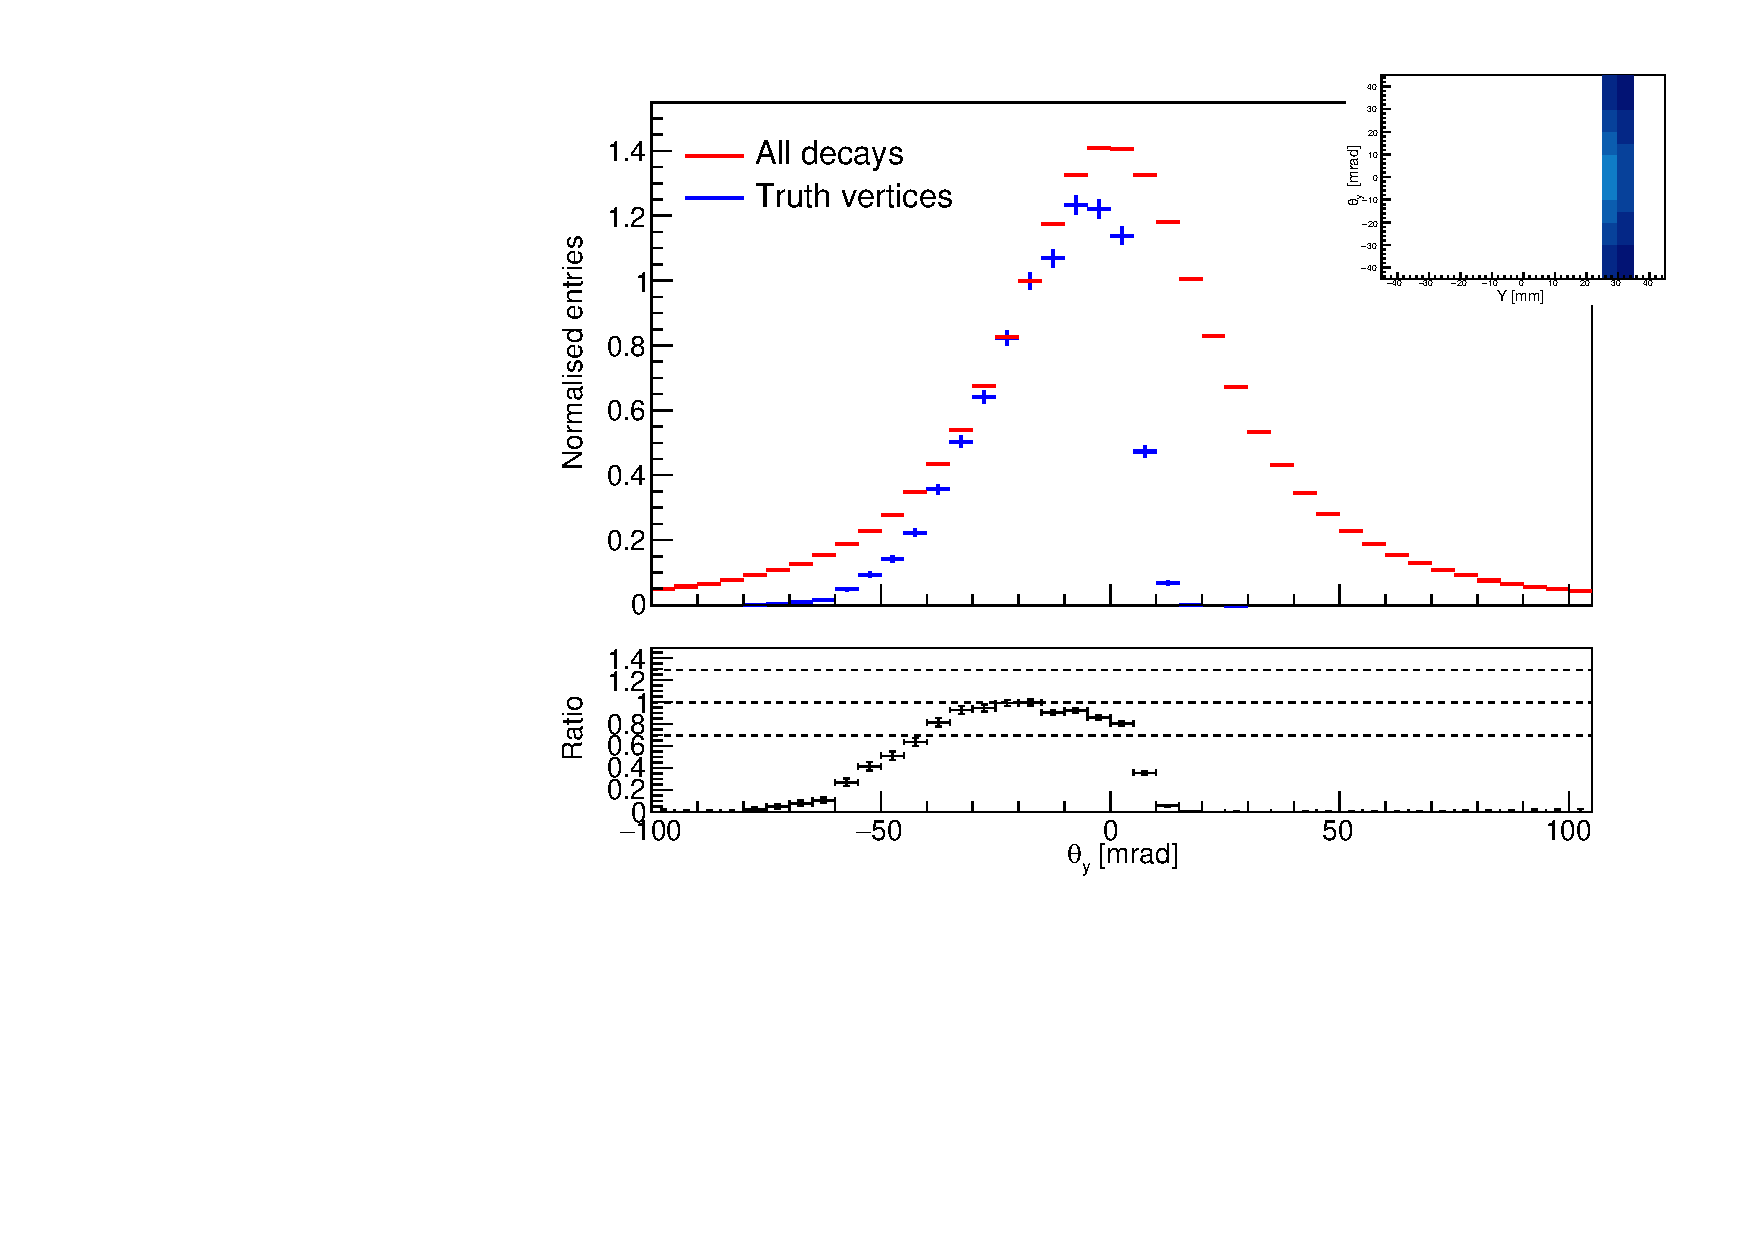
\includegraphics[trim={0 0 0 0},clip,width=.33\textwidth]{Images/Chapter5/S12S18_VerticalDecayAngleRatio_25_35.pdf}}
% \subfloat[]{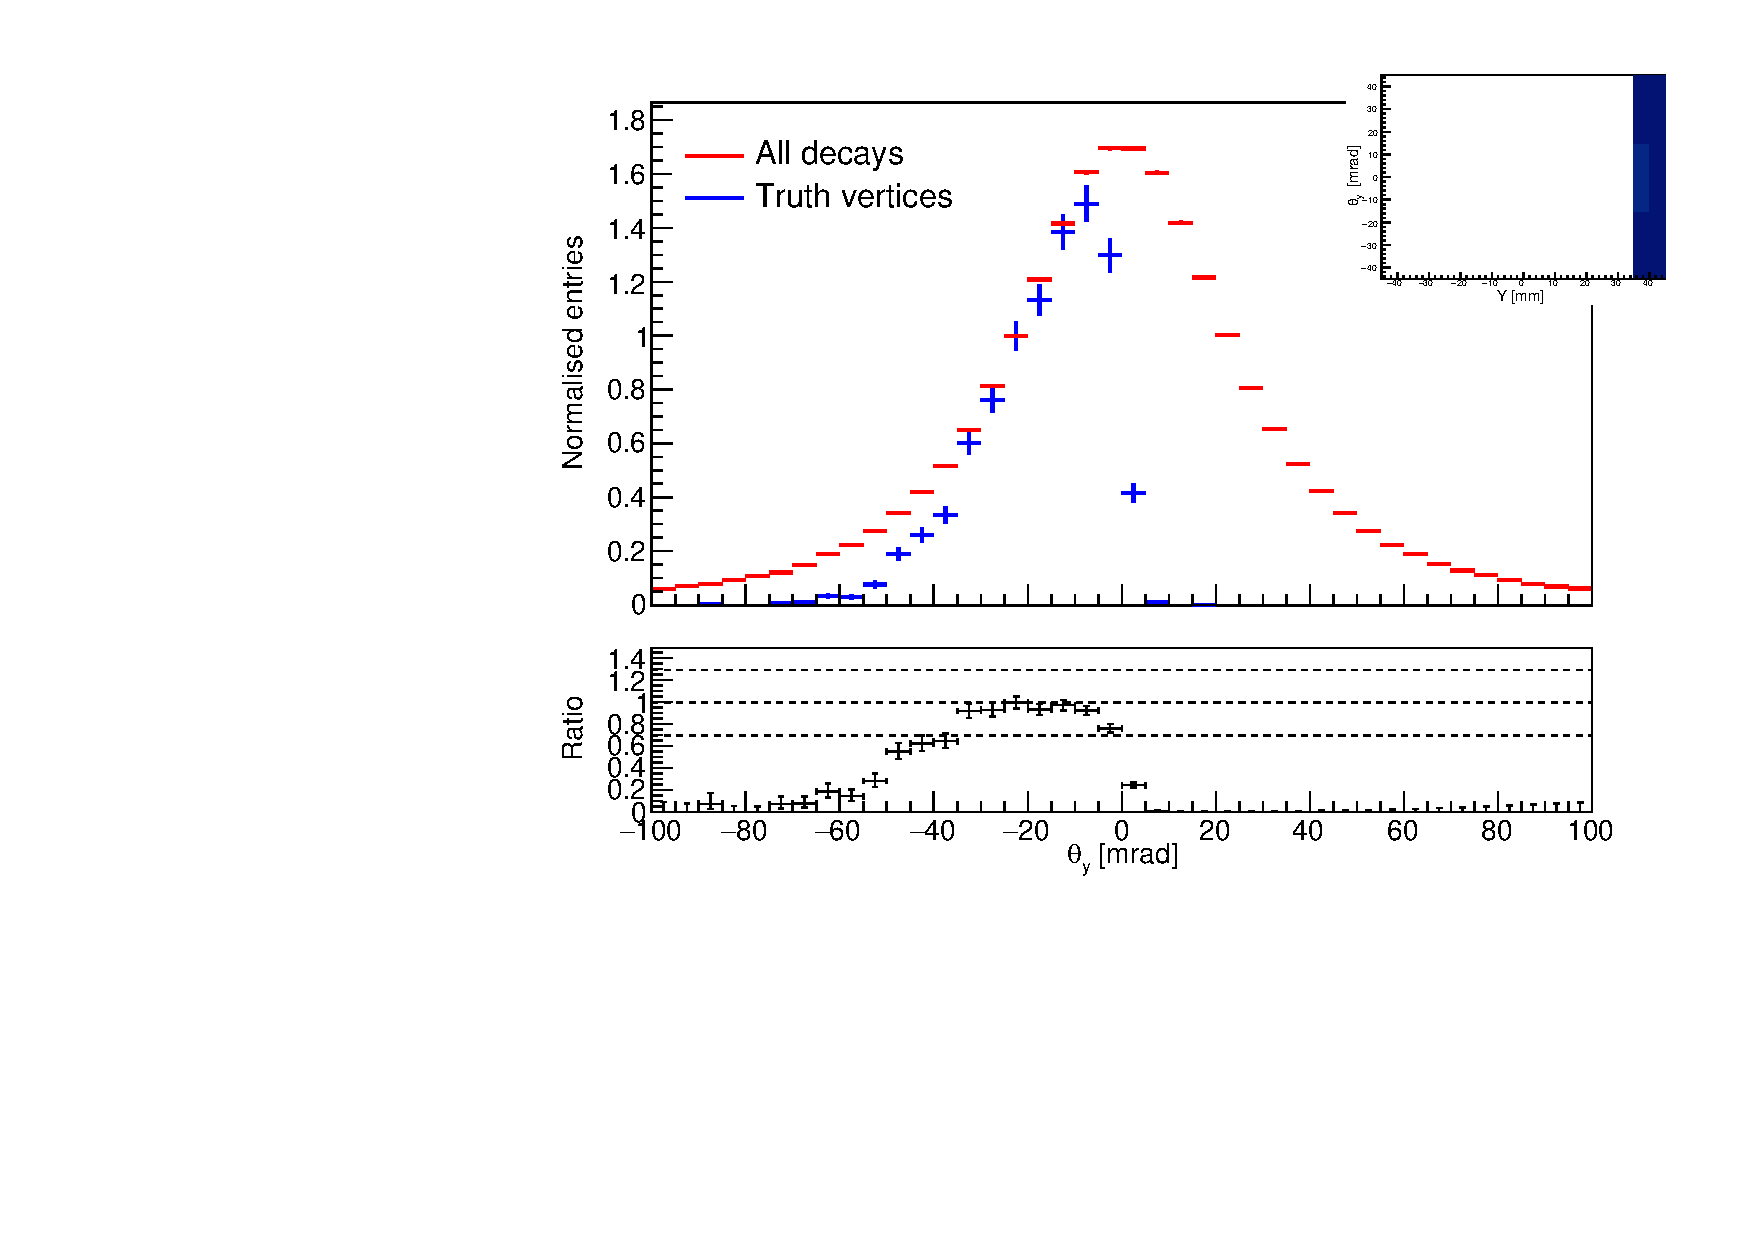
\includegraphics[trim={0 0 0 0},clip,width=.33\textwidth]{Images/Chapter5/S12S18_VerticalDecayAngleRatio_35_45.pdf}}
% \caption{$\theta_{y}$ acceptance ratios in $y$ intervals of \SI{10}{\milli\metre}, indicated by secondary two-dimensional histograms. Positrons originating from the bottom of the storage region must carry a positive vertical component of momentum to be accepted by the straw trackers, and vice versa, resulting in negative correlation between $\theta_{y}$ and $y$. Histograms are formed from a Monte Carlo sample where vertices are a subset of decays, the one-dimensional distributions are normalised to their maximum ratio, and tracker stations are combined.} 
% \label{fig:1DAcceptanceRatios}
% \end{figure} 

The physical origin for the correlation between the accepted $\theta_{y}$ and $y$ is as follows: a positron originating from the bottom of the storage region, vertically lower than the mid-plane of the straw trackers, must possess a positive vertical component of momentum if it is to travel upwards and be accepted by the detector. The reverse is true for positrons originating at the top of the storage region. This effect is demonstrated by Figure \ref{fig:1DAcceptanceRatios}, where one-dimensional distributions of $\theta_{y}$ for \textit{truth vertices} and \textit{all decays} are overlaid in \SI{15}{\milli\metre} intervals of $y$. The physical (\textit{all decays}) distributions of $\theta_{y}$ remains symmetrical, whereas the accepted (\textit{truth vertices}) distribution is positive for a negative interval of $y$, and vice versa. 

The distributions in Figure \ref{fig:1DAcceptanceRatios} are formed from an additional, pre-existing, sample of Monte Carlo with no injected EDM. In this sample, the true extrapolated track vertices are a subset of the truth decay parameters, which is essential when calculating the fraction of decays accepted by the trackers, and is not the case for the simulation datasets detailed in the earlier sections of this chapter. 

\subsection{Acceptance weightings}\label{sec:AcceptanceWeightings}

In order to assess the contribution of acceptance to the reduction of $A_{\text{EDM}}$ between \textit{truth/reco vertices} and \textit{all decays}, shown in Figure \ref{subfig:AEDM_overlay_sim}, the underlying histograms of $\theta_{y}(t)$ used to form the \textit{all decays} vertical angle fits were weighted according to tracker `acceptance maps' in $\theta_{y}$ versus $y$. This weighting procedure corrects the shape of the distribution of $\theta_{y}$, so that \textit{all decays} resembles \textit{truth/reco vertices}, albeit with a different normalisation; however, in the context of this study, the normalisation of $\theta_{y}$ is not relevant. The weighted \textit{all decays} distributions were then fitted for $A_{\text{EDM}}$, and results were compared with those measured from \textit{truth vertices}.% If the two sets of results are consistent, then the vertical acceptance of $\theta_{y}$ can be assumed to be the driving factor in aforementioned additional reduction of $A_{\text{EDM}}$.

\begin{figure}[t!]
\centering{}
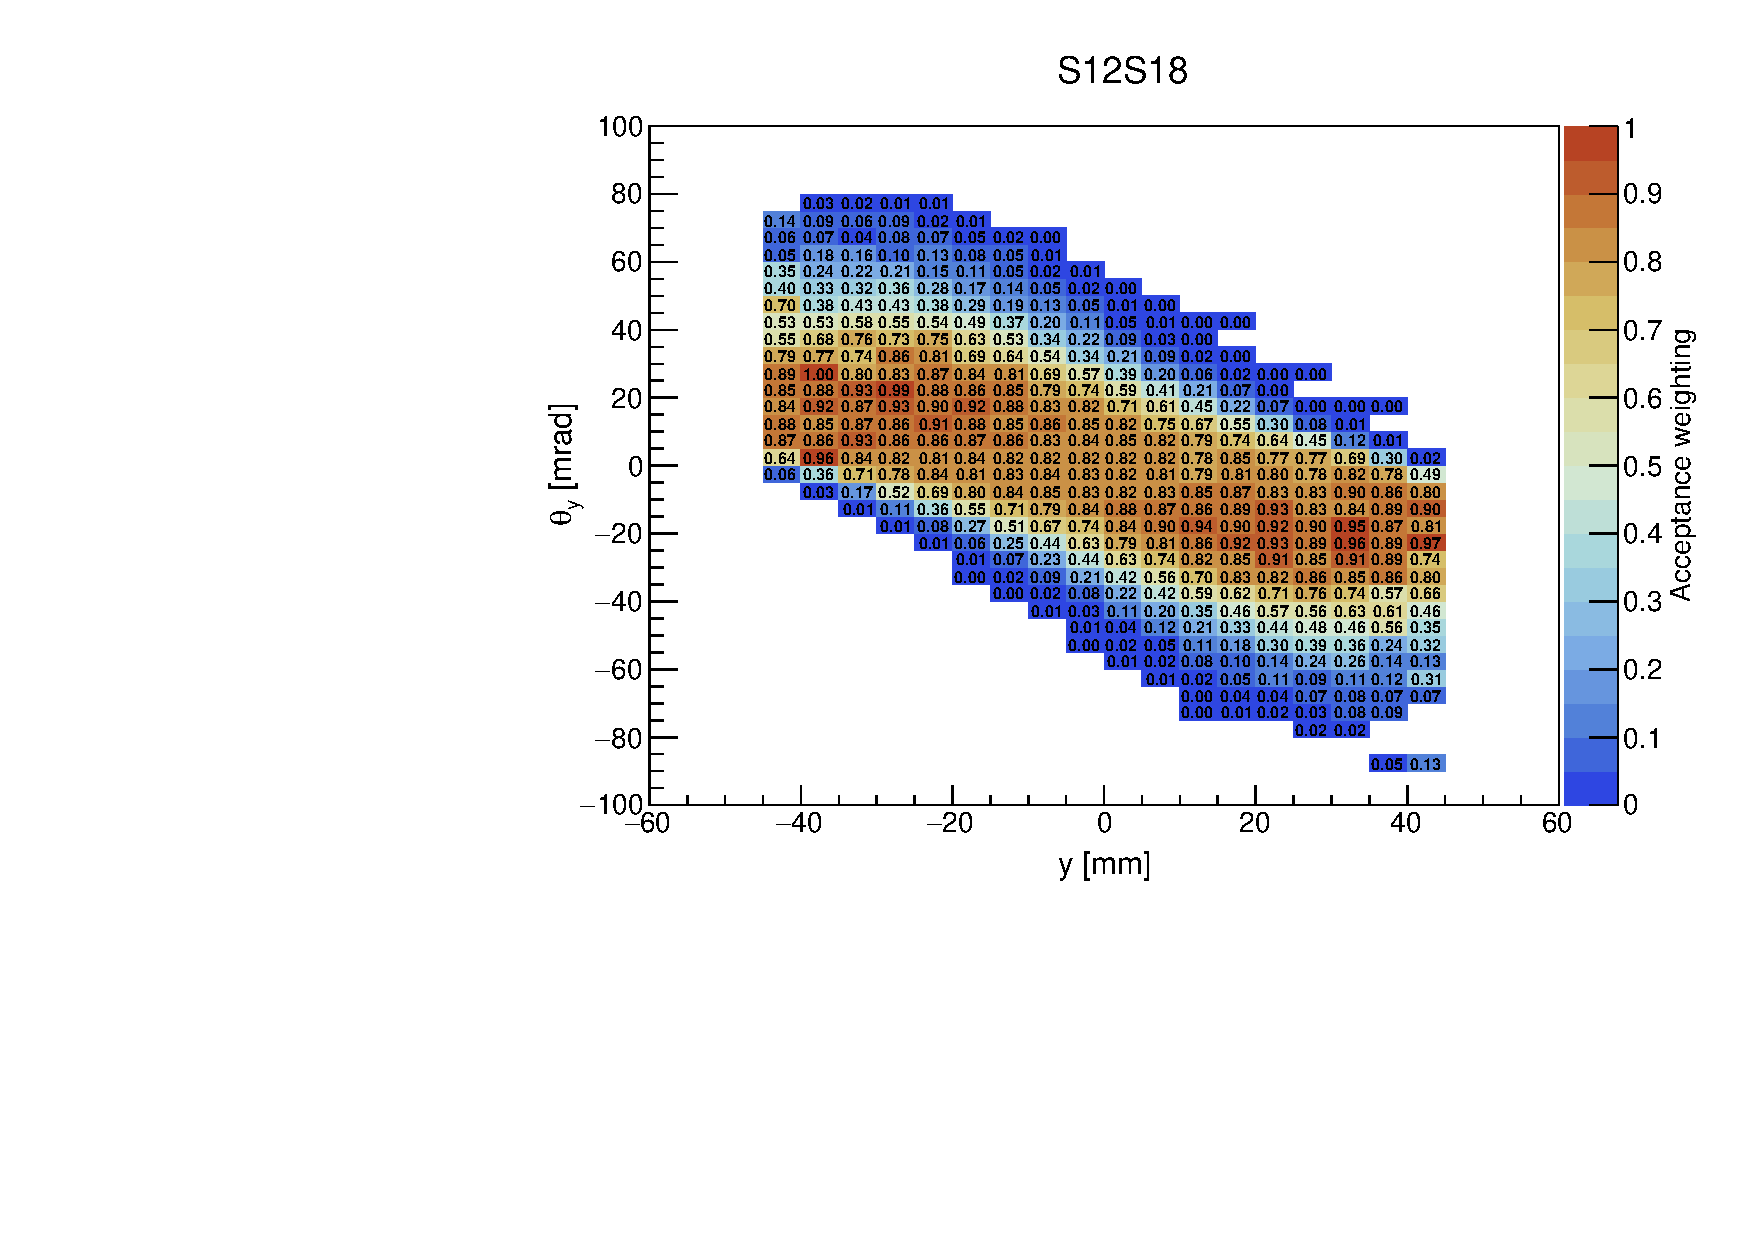
\includegraphics[trim={0 0 0 1cm},clip,width=.69\textwidth]{Images/Chapter5/S12S18_AcceptanceMapY_0_3127_MeV.pdf}
\caption{An acceptance map for all momentum, with tracker stations 12 and 18 combined.}
\label{fig:S12S18_AcceptanceMapY_0_3127_MeV}
\end{figure}

Acceptance weightings were calculated by populating histograms of $\theta_{y}$ against $y$, once for \textit{truth vertices} and then again for \textit{all decays}, using the Monte Carlo sample with no injected EDM. The ratio of these two histograms, after being normalised according to the contents of its maximum bin, gives the aforementioned `acceptance map': a two-dimensional distribution that may be used to weight $\theta_{y}$ according to $y$ for that decay. An example acceptance map for stations 12 and 18 over all momentum is given in Figure \ref{fig:S12S18_AcceptanceMapY_0_3127_MeV}. 

In keeping with the momentum-binned method, treating each momentum interval as an independent analysis, maps were also produced in intervals of 250 MeV, with the \textit{all decays} $\theta_{y}(t)$ distributions per bin being weighted according to the corresponding map for that momentum range. This approach also absorbs acceptance variations along the azimuthal axis, since the average momentum of accepted tracks is positively correlated with track extrapolation distance; that is, tracks originating from further away tend to possess a higher momentum, since low momentum positrons are more likely to curl out of the ring before reaching the detector. Acceptance maps were also produced for individual stations.

Distributions of $A_{\text{EDM}}$ derived from both unweighted and weighted \textit{all decays} samples, as well as \textit{truth vertices}, are shown in momentum intervals of 250 MeV in Figure \ref{fig:AcceptanceCorrected_AEDM_vs_p_overlay}. As an estimate of the level of agreement between the weighted \textit{all decays} distribution and the \textit{truth vertices} distribution, the average number of standard deviations separating the data-points was found to be 1.13, 1.37, and 1.33 for stations 12, 18, and both stations combined respectively. This level of consistency indicates that the reduction of $A_{\text{EDM}}$ measured by the trackers compared to \textit{all decays} may be attributed to tracker acceptance.  

\begin{figure}[t!]
\centering{}
\subfloat[Station 12.]{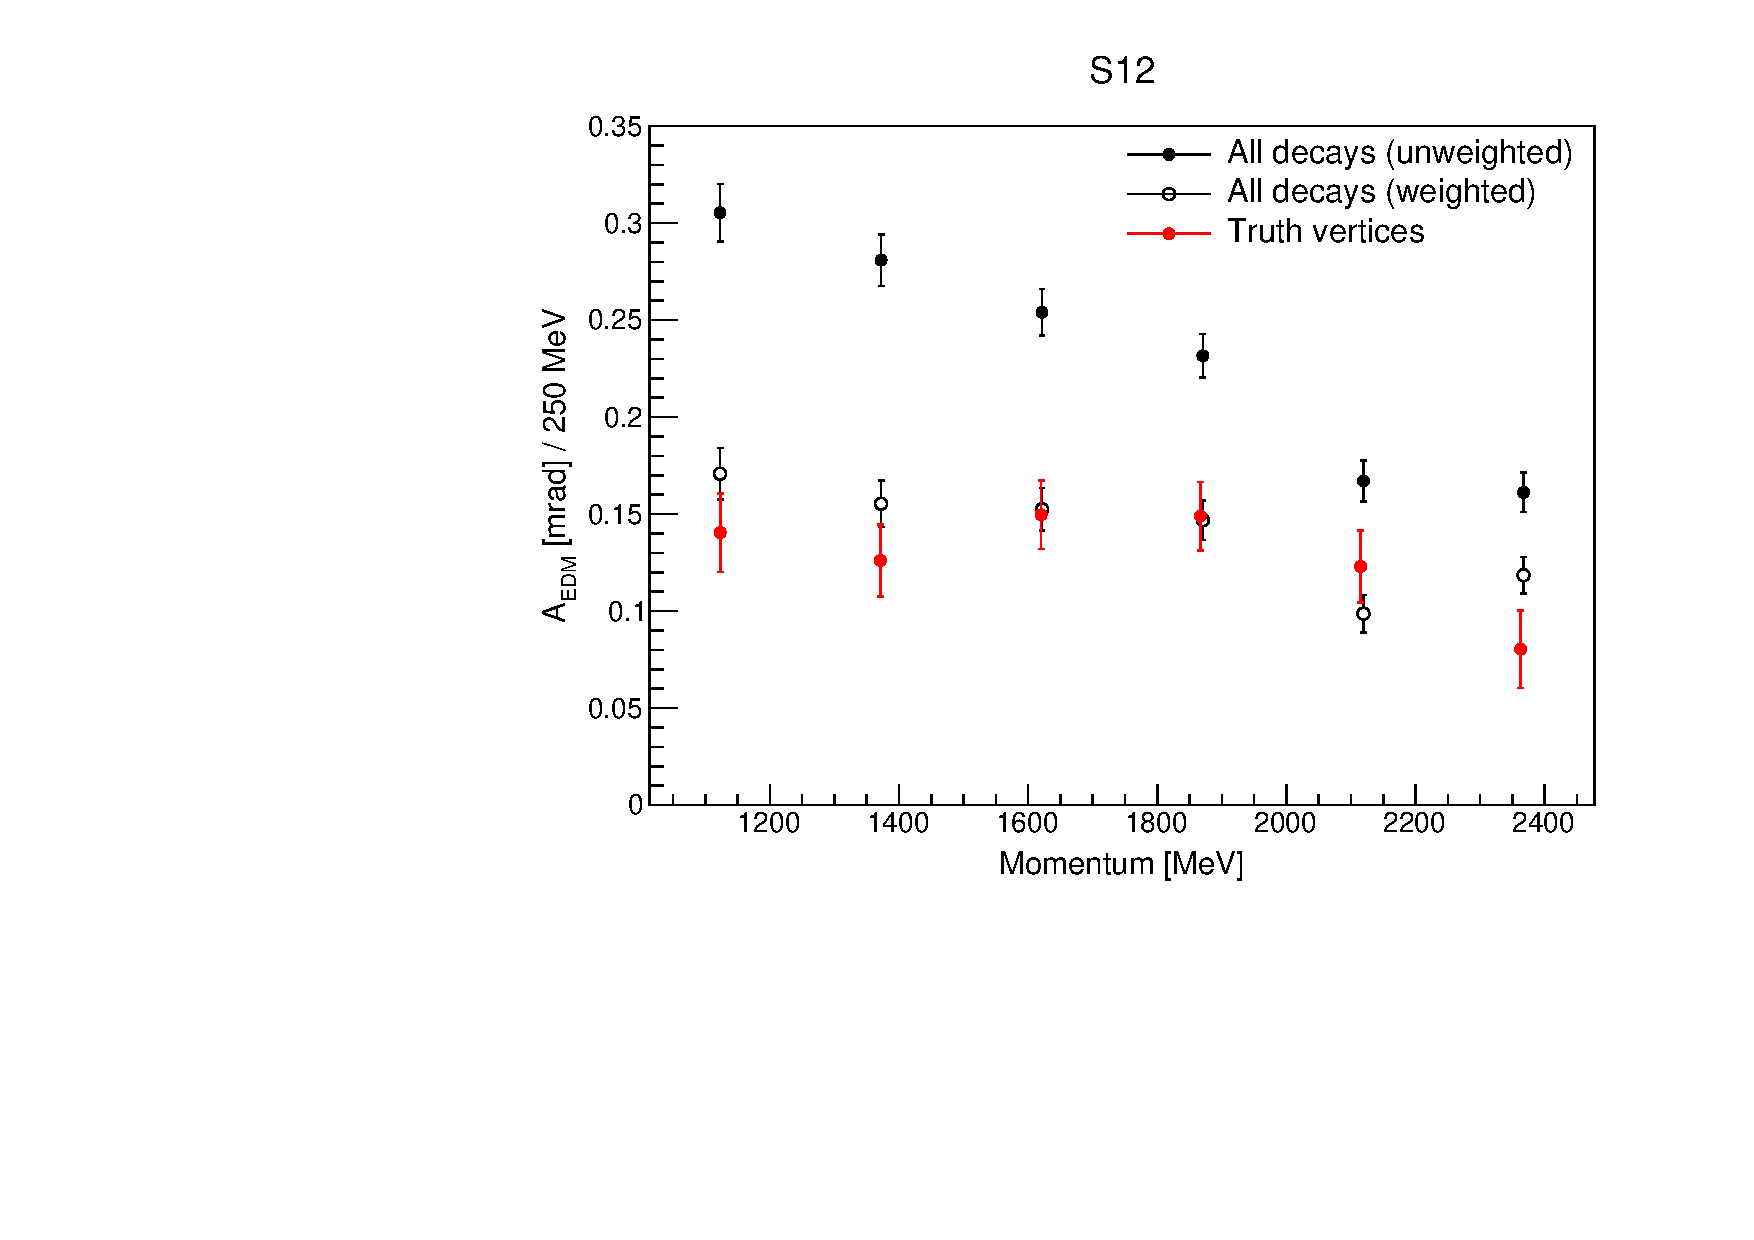
\includegraphics[trim={0 0 0 1cm},clip,width=.49\textwidth]{Images/Chapter5/S12_AcceptanceCorrected_AEDM_vs_p_overlay.pdf}}
\subfloat[Station 18.]{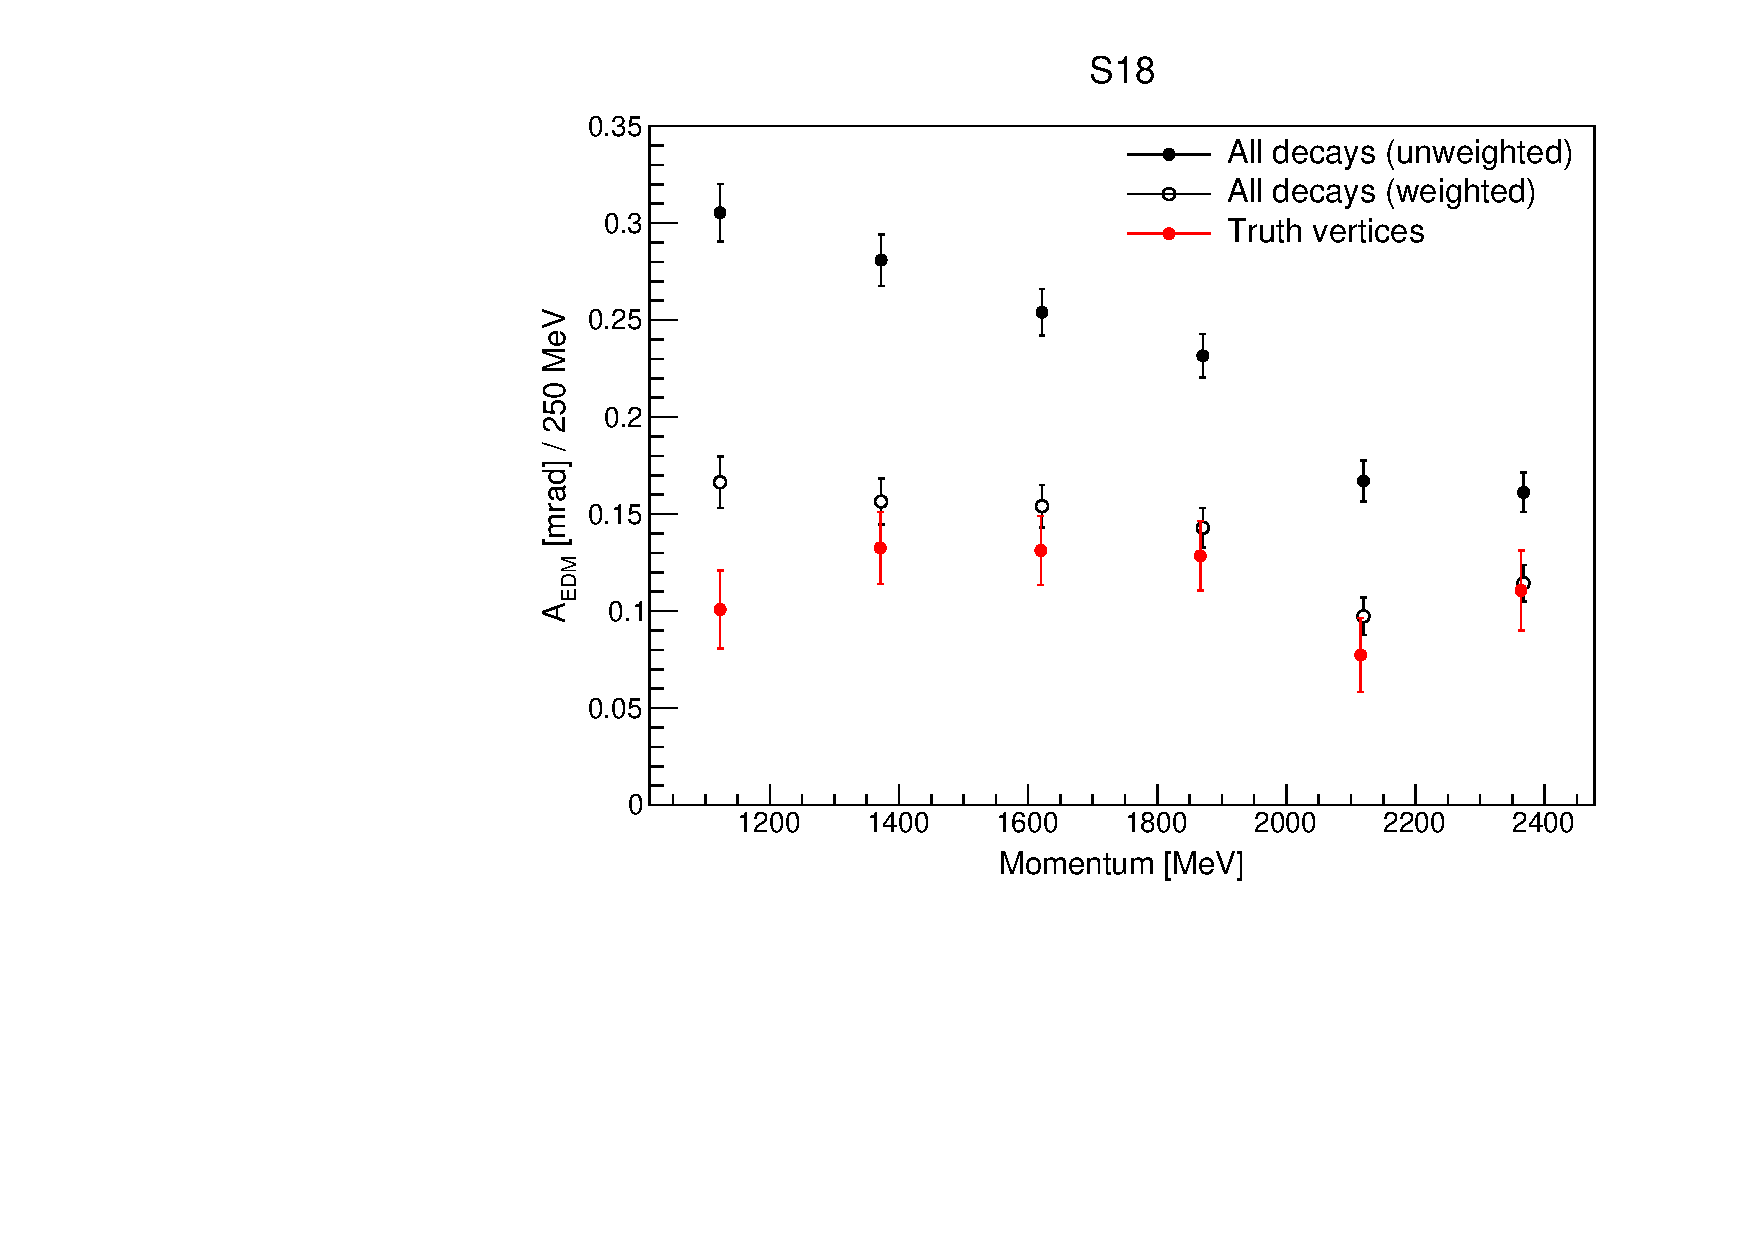
\includegraphics[trim={0 0 0 1cm},clip,width=.49\textwidth]{Images/Chapter5/S18_AcceptanceCorrected_AEDM_vs_p_overlay.pdf}}\hfill
\subfloat[Combined.]{\includegraphics[trim={0 0 0 1cm},clip,width=.69\textwidth]{Images/Chapter5/S12S18_AcceptanceCorrected_AEDM_vs_p_overlay.pdf}}
\caption{Distributions of $A_{\text{EDM}}$ for \textit{all decays}, acceptance weighted \textit{all decays}, and the \textit{truth vertices}. As discussed in the text, the acceptance weighted \textit{all decays} distribution and the \textit{truth vertices} distributions show a good level of consistency, indicating that the observed difference between $A_{\text{EDM}}$ measured from \textit{all decays} compared to \textit{truth vertices} may be attributed to acceptance. Tracker stations 12 and 18 are combined.} 
\label{fig:AcceptanceCorrected_AEDM_vs_p_overlay}
\end{figure} 

\pagebreak

\subsection{The acceptance dilution factor and associated uncertainty}\label{sec:AcceptDilFactor}

Having established that the reduction of $A_{\text{EDM}}$ measured by the trackers compared to \textit{all decays} may be attributed to tracker acceptance, an `$A_{\text{EDM}}$ acceptance factor' was calculated per momentum bin from the ratio of $A_{\text{EDM}}$ measured using \textit{truth vertices} to that measured from \textit{all decays}. These factors may be defined as the tilt angle dilution factors associated with tracker acceptance. 

As shown by Figure \ref{fig:AcceptanceFactor}, the acceptance factors per momentum bin have an associated statistical uncertainty, which arises from the finite Monte Carlo dataset used to determine said factors. To estimate the corresponding uncertainty on the dilution corrected $\delta$, 1000 sets of acceptance factors were randomly drawn from a Gaussian distribution with a mean equal to the acceptance factor in that bin and a width equal to its statistical uncertainty. Each set of acceptance factors is then used to correct the dilution of $A_{\text{EDM}}$ for $\delta$, using a method described in the following section, where the width of the resulting distribution of tilt angles is taken as the uncertainty in units of mrad. This is demonstrated in Figure \ref{fig:AcceptanceStatError}.

\begin{figure}[t!]
\centering{}
\includegraphics[trim={0 0 0 0},clip,width=.69\textwidth]{Images/Chapter5/OverlayMainAcceptanceWeightingVsMomentum.pdf}
\caption{Acceptance factors versus momentum, or the tilt angle dilution factors associated with tracker acceptance, calculated from the ratio of $A_{\text{EDM}}$ measured using \textit{truth vertices} to that measured using \textit{all decays}.} 
\label{fig:AcceptanceFactor}
\end{figure} 
  
\begin{figure}[t!]
\centering{}
\subfloat[]{\includegraphics[trim={0 0 0 1cm},clip,width=.49\textwidth]{Images/Chapter5/S12S18_TrialsOverlay_AcceptanceWeightingVsMomentum.pdf}}
\subfloat[]{\includegraphics[trim={0 0 0 1cm},clip,width=.49\textwidth]{Images/Chapter5/S12S18_EDM_delta_prime_hist_1000_1000-2500MeV_trackReco_WORLD_250MeV_BQ_noVertCorr.pdf}}
\caption{Characterisation of the Monte Carlo statistical uncertainty associated with the dilution corrected tilt angle, showing: (a) 1000 sets of acceptance factors, drawn from Gaussian distributions with a width equal to the statistical uncertainty on the central value; (b) the distribution of dilution corrected tilt angles for measured track vertices, where the width is taken as the uncertainty in mrad.} 
\label{fig:AcceptanceStatError}
\end{figure} 

\section{Extracting the tilt angle}\label{sec:ExtractTiltSim}

\begin{figure}[b!]
\centering{}
\subfloat[]{\includegraphics[trim={0 0 0 0},clip,width=.49\textwidth]{Images/Chapter5/edm_delta_vs_p_30x_allDecays_WORLD_250MeV_AQ.pdf}\label{subfig:30xAllDecaysDeltaVsP}}
\subfloat[]{\includegraphics[trim={0 0 0 0},clip,width=.49\textwidth]{Images/Chapter5/edm_delta_vs_p_10x_allDecays_WORLD_250MeV_AQ.pdf}\label{subfig:10xAllDecaysDeltaVsP}}
\hfill
\subfloat[]{\includegraphics[trim={0 0 0 0},clip,width=.49\textwidth]{Images/Chapter5/S12S18_EDM_delta_prime_vs_p_trackTruth_WORLD_250MeV_BQ_noVertCorr.pdf}\label{subfig:30xTrackTruthDeltaVsP}}
\subfloat[]{\includegraphics[trim={0 0 0 0},clip,width=.49\textwidth]{Images/Chapter5/S12S18_EDM_delta_prime_vs_p_trackReco_WORLD_250MeV_BQ_noVertCorr.pdf}\label{subfig:30xTrackRecoDeltaVsP}}\hfill
\caption{The dilution corrected $\delta$ per 250 MeV momentum bin, for: (a) \textit{all decays} with a 30$\times$ BNL injected EDM, or a 1.69 mrad tilt; (b) \textit{all decays} with a 10$\times$ BNL injected EDM, or a 0.594 mrad tilt; (c) \textit{truth vertices}; and (d) \textit{reco vertices}. Figures (c) and (d) both contain an injected 1.69 mrad tilt, and utilise the $A_{\text{EDM}}$ acceptance factors shown in Figure \ref{fig:AcceptanceFactor}. Tracker stations 12 and 18 are combined. All results are consistent with the injected tilt angle.}
\label{fig:DeltaResultsSim}
\end{figure}

In order to extract the laboratory frame tilt angle, $\delta$, from $A_{\text{EDM}}$ at a particular momentum interval, a correction must be applied which is specific to the average momentum of that interval. In the case of 100\% acceptance (\textit{all decays}), the correction factor may be found by simple evaluation of the dilution function, Equation \ref{eqn:DilutionFunction2}. In the case where tracker acceptance is included (\textit{truth/reco vertices}), the correction factor is the product of the value obtained from the dilution function and the appropriate $A_{\text{EDM}}$ acceptance factor. 

Once the correction factors are applied, the result is a flat distribution of $\delta$ across momentum, which may be fitted with a zeroth order polynomial to obtain an uncertainty weighted average, $\langle \delta \rangle$. As illustrated in Figure \ref{fig:DeltaResultsSim}, this procedure was performed for both the 30$\times$ and 10$\times$ BNL \textit{all decays} samples, which have injected tilt angles of 1.69 mrad and 0.595 mrad respectively, along with the \textit{truth/reco vertices} 30$\times$ BNL samples. Two injected EDM signals were used for purposes of checking for non-linearities between the level of dilution and the size of the injected signal, a possibility which is ruled out by the fact that all measured values of $\langle \delta \rangle$ are consistent with the injected tilt angle. Some deviation is observed at 2000-2250 MeV in all four distributions shown in Figure \ref{fig:DeltaResultsSim}, which may be entirely attributed to a statistical fluctuation at the same momentum interval in Figure \ref{subfig:AllDecaysFit}.

\section{Tracker global alignment characterisation}\label{sec:Alignment}

The characterisation of acceptance, described in the previous section, relies on the simulated detectors being orientated at the same relative position to the beam as in data. If this is not the case, then the acceptance correction uncertainty will receive some systematic contribution according to the size of the misalignment. In this section, a preliminary procedure for determining the size of this contribution from the straw tracker global alignment\footnote{Global alignment refers to the absolute position of the tracker stations in the experiment’s global coordinate system. This is distinct from internal alignment, which pertains to the relative position of the individual tracker modules. Alignment is discussed in detail in \cite{Lukicov}.} error, in terms of an uncertainty on $\langle \delta \rangle$, will be described. 

\begin{figure}[b!]
\centering{}
\subfloat[Station 12 ($+1$ mm).]{\includegraphics[trim={0 0 0 1cm},clip,width=.49\textwidth]{Images/Chapter5/S12_AlignmentShifted_AEDM_vs_p_overlay.pdf}}
\subfloat[Station 18 ($-1$ mm).]{\includegraphics[trim={0 0 0 1cm},clip,width=.49\textwidth]{Images/Chapter5/S18_AlignmentShifted_AEDM_vs_p_overlay.pdf}}
\caption{Distributions of $A_{\text{EDM}}$ with the tracker global vertical position shifted by (a) $+1$ mm for station 12 and (b) $-1$ mm for station 18, using the \textit{truth vertices} reconstruction. Also shown is the nominal distribution from the \textit{all decays} reconstruction.} 
\label{fig:AEDMWithAlignment}
\end{figure}   

The straw tracker global alignment, hereafter referred to as `alignment', has four parameters: the radial position, vertical position, radial angle, and vertical angle. These parameters are precisely measured via laser survey \cite{Lukicov}, with an uncertainty associated with each. In the context of the vertical $\theta_{y}$ acceptance uncertainty, the most relevant parameters are the vertical position and vertical angle. In the following preliminary study, only the vertical position, which has an uncertainty of $\pm0.6$ mm \cite{VerticalGlobalAlignment}, is considered. 

\begin{figure}[t!]
\centering{}
\includegraphics[trim={0 0 0 0cm},clip,width=.69\textwidth]{Images/Chapter5/AEDMAcceptanceUncOverlay.pdf}
\caption{The variation in $A_{\text{EDM}}$ acceptance factor with the tracker global vertical position shifted by $\pm1$ mm.} 
\label{fig:AEDMAlignmentUnc}
\end{figure} 

In order to begin propagating the vertical position alignment error through to an uncertainty on $\langle \delta \rangle$, the vertical alignment parameter was varied in simulation and the resulting shift in $A_{\text{EDM}}$ was measured. In each case, the vertical position alignment was varied by $+1$ mm for station 12 and $-1$ mm for station 18. Due to practical constraints, only a subset of the sample described in Section \ref{sec:SimulatingALargeEDM} was available for reconstruction, which manifests an increased statistical uncertainty on $A_{\text{EDM}}$. The resulting distributions of $A_{\text{EDM}}$ against momentum are shown in Figure \ref{fig:AEDMWithAlignment}. 

The change in the $A_{\text{EDM}}$ acceptance factor per mm is then approximated by subtracting the factors calculated at nominal vertical alignment from those calculated at $\pm1$ mm vertical alignment, shown in Figure \ref{fig:AEDMAlignmentUnc}. This uncertainty may then be estimated in terms of $\langle \delta \rangle$ by varying the nominal acceptance factor according to aforementioned $\pm0.6$ mm uncertainty, and taking the average shift in $\langle \delta \rangle$ as the uncertainty. 

The procedure described in this section makes the approximation that the uncertainties associated with $A_{\text{EDM}}$ are 100\% correlated between the nominal and shifted samples, that is, the sets of tracks in both samples are derived from the same set of positrons. This is an inaccuracy, although the exact level of correlation is not known at present, and so the possibility that the variation seen in Figures \ref{fig:AEDMWithAlignment} and \ref{fig:AEDMAlignmentUnc} is due to statistical fluctuations cannot be excluded. Because of this, and the fact that the contributions from the global tracker vertical angle is not yet included, the global alignment uncertainty described here must be considered preliminary. 

\section{Summary and outlook}

% In summary, a large-scale sample of Monte Carlo with a injected muon EDM signal of $5.4\times10^{-18}$ $e\cdot$cm (30$\times$ the BNL upper limit \cite{BNLEDM}), was generated. 

% Chapter \ref{chap:5} describes the large-scale simulation efforts which are essential to the development and proving characterisation of sources of systematic uncertainty in the measurement, and, critically, the contribution from detector acceptance to the observed momentum dependent dilution of the EDM signal.

The large-scale Monte Carlo simulation efforts outlined in this chapter have been shown to be vital to the development and verification of the tracker-based muon EDM analysis technique. The analysis procedure was demonstrated by use of a primary sample with an injected EDM of $5.4\times10^{-18}$ $e\cdot$cm (30$\times$ the BNL upper limit \cite{BNLEDM}), and a secondary sample with an injected EDM of $1.8\times10^{-18}$ (10$\times$ BNL). The momentum-binned approach to fitting the vertical angle oscillation was introduced and motivated, based on the variation of $\langle \theta_{y} \rangle$, and the dilution of $\delta$, with momentum. The decay asymmetry and dilution functions, Equations \ref{eqn:AEDM_labFrame} and \ref{eqn:DilutionFunction2}, were verified, and the impact of tracker acceptance on the dilution of observed angle $A_{\text{EDM}}$ was characterised. Critically, this enables $\delta$ to be extracted from the measured $A_{\text{EDM}}$, producing results consistent with expectation, as shown. Finally, procedures were developed for estimating the contributions to the uncertainty on $\delta$ from the acceptance correction, including the contribution from the Monte Carlo statistical uncertainty, and, preliminarily, the contribution from global vertical alignment. 

Moving forward, a greater number of events will be folded into the Monte Carlo datasets used to characterise the contribution from tracker acceptance to the dilution of $\delta$, thereby reducing the statistical uncertainty associated with the $A_{\text{EDM}}$ acceptance factors, and assisting in the analysis of the global alignment uncertainty. Additionally, the variation in $A_{\text{EDM}}$ arising from the tracker vertical tilt angle error will be incorporated into said alignment uncertainty.